\documentclass[twoside]{book}

% Packages required by doxygen
\usepackage{calc}
\usepackage{doxygen}
\usepackage{graphicx}
\usepackage[utf8]{inputenc}
\usepackage{makeidx}
\usepackage{multicol}
\usepackage{multirow}
\usepackage{textcomp}
\usepackage[table]{xcolor}

% Font selection
\usepackage[T1]{fontenc}
\usepackage{mathptmx}
\usepackage[scaled=.90]{helvet}
\usepackage{courier}
\usepackage{amssymb}
\usepackage{sectsty}
\renewcommand{\familydefault}{\sfdefault}
\allsectionsfont{%
  \fontseries{bc}\selectfont%
  \color{darkgray}%
}
\renewcommand{\DoxyLabelFont}{%
  \fontseries{bc}\selectfont%
  \color{darkgray}%
}

% Page & text layout
\usepackage{geometry}
\geometry{%
  a4paper,%
  top=2.5cm,%
  bottom=2.5cm,%
  left=2.5cm,%
  right=2.5cm%
}
\tolerance=750
\hfuzz=15pt
\hbadness=750
\setlength{\emergencystretch}{15pt}
\setlength{\parindent}{0cm}
\setlength{\parskip}{0.2cm}
\makeatletter
\renewcommand{\paragraph}{%
  \@startsection{paragraph}{4}{0ex}{-1.0ex}{1.0ex}{%
    \normalfont\normalsize\bfseries\SS@parafont%
  }%
}
\renewcommand{\subparagraph}{%
  \@startsection{subparagraph}{5}{0ex}{-1.0ex}{1.0ex}{%
    \normalfont\normalsize\bfseries\SS@subparafont%
  }%
}
\makeatother

% Headers & footers
\usepackage{fancyhdr}
\pagestyle{fancyplain}
\fancyhead[LE]{\fancyplain{}{\bfseries\thepage}}
\fancyhead[CE]{\fancyplain{}{}}
\fancyhead[RE]{\fancyplain{}{\bfseries\leftmark}}
\fancyhead[LO]{\fancyplain{}{\bfseries\rightmark}}
\fancyhead[CO]{\fancyplain{}{}}
\fancyhead[RO]{\fancyplain{}{\bfseries\thepage}}
\fancyfoot[LE]{\fancyplain{}{}}
\fancyfoot[CE]{\fancyplain{}{}}
\fancyfoot[RE]{\fancyplain{}{\bfseries\scriptsize Generated on Mon Jul 28 2014 06\-:09\-:29 for Network traffic simulator by Doxygen }}
\fancyfoot[LO]{\fancyplain{}{\bfseries\scriptsize Generated on Mon Jul 28 2014 06\-:09\-:29 for Network traffic simulator by Doxygen }}
\fancyfoot[CO]{\fancyplain{}{}}
\fancyfoot[RO]{\fancyplain{}{}}
\renewcommand{\footrulewidth}{0.4pt}
\renewcommand{\chaptermark}[1]{%
  \markboth{#1}{}%
}
\renewcommand{\sectionmark}[1]{%
  \markright{\thesection\ #1}%
}

% Indices & bibliography
\usepackage{natbib}
\usepackage[titles]{tocloft}
\setcounter{tocdepth}{3}
\setcounter{secnumdepth}{5}
\makeindex

% Hyperlinks (required, but should be loaded last)
\usepackage{ifpdf}
\ifpdf
  \usepackage[pdftex,pagebackref=true]{hyperref}
\else
  \usepackage[ps2pdf,pagebackref=true]{hyperref}
\fi
\hypersetup{%
  colorlinks=true,%
  linkcolor=blue,%
  citecolor=blue,%
  unicode%
}

% Custom commands
\newcommand{\clearemptydoublepage}{%
  \newpage{\pagestyle{empty}\cleardoublepage}%
}


%===== C O N T E N T S =====

\begin{document}

% Titlepage & ToC
\hypersetup{pageanchor=false}
\pagenumbering{roman}
\begin{titlepage}
\vspace*{7cm}
\begin{center}%
{\Large Network traffic simulator \\[1ex]\large 1.\-0 }\\
\vspace*{1cm}
{\large Generated by Doxygen 1.8.6}\\
\vspace*{0.5cm}
{\small Mon Jul 28 2014 06:09:29}\\
\end{center}
\end{titlepage}
\clearemptydoublepage
\tableofcontents
\clearemptydoublepage
\pagenumbering{arabic}
\hypersetup{pageanchor=true}

%--- Begin generated contents ---
\chapter{Namespace Index}
\section{Namespace List}
Here is a list of all namespaces with brief descriptions\-:\begin{DoxyCompactList}
\item\contentsline{section}{\hyperlink{namespaceMFF__NPRG031}{M\-F\-F\-\_\-\-N\-P\-R\-G031} }{\pageref{namespaceMFF__NPRG031}}{}
\item\contentsline{section}{\hyperlink{namespaceNetTrafficSimulator}{Net\-Traffic\-Simulator} }{\pageref{namespaceNetTrafficSimulator}}{}
\item\contentsline{section}{\hyperlink{namespaceStetic}{Stetic} }{\pageref{namespaceStetic}}{}
\end{DoxyCompactList}

\chapter{Hierarchical Index}
\section{Class Hierarchy}
This inheritance list is sorted roughly, but not completely, alphabetically\-:\begin{DoxyCompactList}
\item \contentsline{section}{M\-F\-F\-\_\-\-N\-P\-R\-G031.\-Calendar}{\pageref{classMFF__NPRG031_1_1Calendar}}{}
\item \contentsline{section}{Net\-Traffic\-Simulator.\-Link.\-Data\-Envelope}{\pageref{classNetTrafficSimulator_1_1Link_1_1DataEnvelope}}{}
\item \contentsline{section}{M\-F\-F\-\_\-\-N\-P\-R\-G031.\-Event}{\pageref{classMFF__NPRG031_1_1Event}}{}
\item \contentsline{section}{Net\-Traffic\-Simulator.\-I\-Addressable}{\pageref{interfaceNetTrafficSimulator_1_1IAddressable}}{}
\begin{DoxyCompactList}
\item \contentsline{section}{Net\-Traffic\-Simulator.\-End\-Node}{\pageref{classNetTrafficSimulator_1_1EndNode}}{}
\item \contentsline{section}{Net\-Traffic\-Simulator.\-Server\-Node}{\pageref{classNetTrafficSimulator_1_1ServerNode}}{}
\end{DoxyCompactList}
\item \contentsline{section}{Net\-Traffic\-Simulator.\-I\-Namable}{\pageref{interfaceNetTrafficSimulator_1_1INamable}}{}
\begin{DoxyCompactList}
\item \contentsline{section}{Net\-Traffic\-Simulator.\-Link}{\pageref{classNetTrafficSimulator_1_1Link}}{}
\item \contentsline{section}{Net\-Traffic\-Simulator.\-Node}{\pageref{classNetTrafficSimulator_1_1Node}}{}
\begin{DoxyCompactList}
\item \contentsline{section}{Net\-Traffic\-Simulator.\-End\-Node}{\pageref{classNetTrafficSimulator_1_1EndNode}}{}
\item \contentsline{section}{Net\-Traffic\-Simulator.\-Network\-Node}{\pageref{classNetTrafficSimulator_1_1NetworkNode}}{}
\item \contentsline{section}{Net\-Traffic\-Simulator.\-Server\-Node}{\pageref{classNetTrafficSimulator_1_1ServerNode}}{}
\end{DoxyCompactList}
\end{DoxyCompactList}
\item \contentsline{section}{Net\-Traffic\-Simulator.\-I\-Result\-Provider}{\pageref{interfaceNetTrafficSimulator_1_1IResultProvider}}{}
\begin{DoxyCompactList}
\item \contentsline{section}{Net\-Traffic\-Simulator.\-End\-Node}{\pageref{classNetTrafficSimulator_1_1EndNode}}{}
\item \contentsline{section}{Net\-Traffic\-Simulator.\-Link}{\pageref{classNetTrafficSimulator_1_1Link}}{}
\item \contentsline{section}{Net\-Traffic\-Simulator.\-Network\-Node}{\pageref{classNetTrafficSimulator_1_1NetworkNode}}{}
\item \contentsline{section}{Net\-Traffic\-Simulator.\-Server\-Node}{\pageref{classNetTrafficSimulator_1_1ServerNode}}{}
\end{DoxyCompactList}
\item \contentsline{section}{Net\-Traffic\-Simulator.\-Main\-Class}{\pageref{classNetTrafficSimulator_1_1MainClass}}{}
\item \contentsline{section}{M\-F\-F\-\_\-\-N\-P\-R\-G031.\-Model}{\pageref{classMFF__NPRG031_1_1Model}}{}
\item \contentsline{section}{Net\-Traffic\-Simulator.\-Network\-Model}{\pageref{classNetTrafficSimulator_1_1NetworkModel}}{}
\item \contentsline{section}{Net\-Traffic\-Simulator.\-Network\-Model\-Test}{\pageref{classNetTrafficSimulator_1_1NetworkModelTest}}{}
\item \contentsline{section}{Net\-Traffic\-Simulator.\-Packet}{\pageref{classNetTrafficSimulator_1_1Packet}}{}
\item \contentsline{section}{M\-F\-F\-\_\-\-N\-P\-R\-G031.\-Process}{\pageref{classMFF__NPRG031_1_1Process}}{}
\begin{DoxyCompactList}
\item \contentsline{section}{Net\-Traffic\-Simulator.\-Link}{\pageref{classNetTrafficSimulator_1_1Link}}{}
\item \contentsline{section}{Net\-Traffic\-Simulator.\-Node}{\pageref{classNetTrafficSimulator_1_1Node}}{}
\end{DoxyCompactList}
\item \contentsline{section}{Net\-Traffic\-Simulator.\-Result\-Model}{\pageref{classNetTrafficSimulator_1_1ResultModel}}{}
\item \contentsline{section}{Net\-Traffic\-Simulator.\-Simulation\-Controller}{\pageref{classNetTrafficSimulator_1_1SimulationController}}{}
\item \contentsline{section}{Net\-Traffic\-Simulator.\-Simulation\-Controller\-Test}{\pageref{classNetTrafficSimulator_1_1SimulationControllerTest}}{}
\item \contentsline{section}{Net\-Traffic\-Simulator.\-Simulation\-Model}{\pageref{classNetTrafficSimulator_1_1SimulationModel}}{}
\item \contentsline{section}{Net\-Traffic\-Simulator.\-Simulation\-Model\-Test}{\pageref{classNetTrafficSimulator_1_1SimulationModelTest}}{}
\item \contentsline{section}{M\-F\-F\-\_\-\-N\-P\-R\-G031.\-State}{\pageref{classMFF__NPRG031_1_1State}}{}
\item Window\begin{DoxyCompactList}
\item \contentsline{section}{Main\-Window}{\pageref{classMainWindow}}{}
\end{DoxyCompactList}
\end{DoxyCompactList}

\chapter{Class Index}
\section{Class List}
Here are the classes, structs, unions and interfaces with brief descriptions\-:\begin{DoxyCompactList}
\item\contentsline{section}{\hyperlink{classNetTrafficSimulator_1_1MainClass}{Net\-Traffic\-Simulator.\-Main\-Class} }{\pageref{classNetTrafficSimulator_1_1MainClass}}{}
\item\contentsline{section}{\hyperlink{classMainWindow}{Main\-Window} }{\pageref{classMainWindow}}{}
\item\contentsline{section}{\hyperlink{classNetTrafficSimulator_1_1NetworkModel}{Net\-Traffic\-Simulator.\-Network\-Model} }{\pageref{classNetTrafficSimulator_1_1NetworkModel}}{}
\item\contentsline{section}{\hyperlink{classNetTrafficSimulator_1_1NetworkModelTest}{Net\-Traffic\-Simulator.\-Network\-Model\-Test} }{\pageref{classNetTrafficSimulator_1_1NetworkModelTest}}{}
\end{DoxyCompactList}

\chapter{File Index}
\section{File List}
Here is a list of all files with brief descriptions\-:\begin{DoxyCompactList}
\item\contentsline{section}{Net\-Traffic\-Simulator/\-Net\-Traffic\-Simulator/\hyperlink{MainWindow_8cs}{Main\-Window.\-cs} }{\pageref{MainWindow_8cs}}{}
\item\contentsline{section}{Net\-Traffic\-Simulator/\-Net\-Traffic\-Simulator/\hyperlink{Program_8cs}{Program.\-cs} }{\pageref{Program_8cs}}{}
\item\contentsline{section}{Net\-Traffic\-Simulator/\-Net\-Traffic\-Simulator/controller/\hyperlink{SimulationController_8cs}{Simulation\-Controller.\-cs} }{\pageref{SimulationController_8cs}}{}
\item\contentsline{section}{Net\-Traffic\-Simulator/\-Net\-Traffic\-Simulator/controller/\hyperlink{SimulationControllerTest_8cs}{Simulation\-Controller\-Test.\-cs} }{\pageref{SimulationControllerTest_8cs}}{}
\item\contentsline{section}{Net\-Traffic\-Simulator/\-Net\-Traffic\-Simulator/framework/\hyperlink{Calendar_8cs}{Calendar.\-cs} }{\pageref{Calendar_8cs}}{}
\item\contentsline{section}{Net\-Traffic\-Simulator/\-Net\-Traffic\-Simulator/framework/\hyperlink{Event_8cs}{Event.\-cs} }{\pageref{Event_8cs}}{}
\item\contentsline{section}{Net\-Traffic\-Simulator/\-Net\-Traffic\-Simulator/framework/\hyperlink{Model_8cs}{Model.\-cs} }{\pageref{Model_8cs}}{}
\item\contentsline{section}{Net\-Traffic\-Simulator/\-Net\-Traffic\-Simulator/framework/\hyperlink{Process_8cs}{Process.\-cs} }{\pageref{Process_8cs}}{}
\item\contentsline{section}{Net\-Traffic\-Simulator/\-Net\-Traffic\-Simulator/framework/\hyperlink{State_8cs}{State.\-cs} }{\pageref{State_8cs}}{}
\item\contentsline{section}{Net\-Traffic\-Simulator/\-Net\-Traffic\-Simulator/framework/extension/\hyperlink{EndNode_8cs}{End\-Node.\-cs} }{\pageref{EndNode_8cs}}{}
\item\contentsline{section}{Net\-Traffic\-Simulator/\-Net\-Traffic\-Simulator/framework/extension/\hyperlink{Link_8cs}{Link.\-cs} }{\pageref{Link_8cs}}{}
\item\contentsline{section}{Net\-Traffic\-Simulator/\-Net\-Traffic\-Simulator/framework/extension/\hyperlink{NetworkNode_8cs}{Network\-Node.\-cs} }{\pageref{NetworkNode_8cs}}{}
\item\contentsline{section}{Net\-Traffic\-Simulator/\-Net\-Traffic\-Simulator/framework/extension/\hyperlink{Node_8cs}{Node.\-cs} }{\pageref{Node_8cs}}{}
\item\contentsline{section}{Net\-Traffic\-Simulator/\-Net\-Traffic\-Simulator/framework/extension/\hyperlink{Packet_8cs}{Packet.\-cs} }{\pageref{Packet_8cs}}{}
\item\contentsline{section}{Net\-Traffic\-Simulator/\-Net\-Traffic\-Simulator/framework/extension/\hyperlink{ServerNode_8cs}{Server\-Node.\-cs} }{\pageref{ServerNode_8cs}}{}
\item\contentsline{section}{Net\-Traffic\-Simulator/\-Net\-Traffic\-Simulator/gtk-\/gui/\hyperlink{generated_8cs}{generated.\-cs} }{\pageref{generated_8cs}}{}
\item\contentsline{section}{Net\-Traffic\-Simulator/\-Net\-Traffic\-Simulator/gtk-\/gui/\hyperlink{gtk-gui_2MainWindow_8cs}{Main\-Window.\-cs} }{\pageref{gtk-gui_2MainWindow_8cs}}{}
\item\contentsline{section}{Net\-Traffic\-Simulator/\-Net\-Traffic\-Simulator/misc/\hyperlink{IAddressable_8cs}{I\-Addressable.\-cs} }{\pageref{IAddressable_8cs}}{}
\item\contentsline{section}{Net\-Traffic\-Simulator/\-Net\-Traffic\-Simulator/misc/\hyperlink{INamable_8cs}{I\-Namable.\-cs} }{\pageref{INamable_8cs}}{}
\item\contentsline{section}{Net\-Traffic\-Simulator/\-Net\-Traffic\-Simulator/misc/\hyperlink{IResultProvider_8cs}{I\-Result\-Provider.\-cs} }{\pageref{IResultProvider_8cs}}{}
\item\contentsline{section}{Net\-Traffic\-Simulator/\-Net\-Traffic\-Simulator/model/\hyperlink{NetworkModel_8cs}{Network\-Model.\-cs} }{\pageref{NetworkModel_8cs}}{}
\item\contentsline{section}{Net\-Traffic\-Simulator/\-Net\-Traffic\-Simulator/model/\hyperlink{NetworkModelTest_8cs}{Network\-Model\-Test.\-cs} }{\pageref{NetworkModelTest_8cs}}{}
\item\contentsline{section}{Net\-Traffic\-Simulator/\-Net\-Traffic\-Simulator/model/\hyperlink{ResultModel_8cs}{Result\-Model.\-cs} }{\pageref{ResultModel_8cs}}{}
\item\contentsline{section}{Net\-Traffic\-Simulator/\-Net\-Traffic\-Simulator/model/\hyperlink{SimulationModel_8cs}{Simulation\-Model.\-cs} }{\pageref{SimulationModel_8cs}}{}
\item\contentsline{section}{Net\-Traffic\-Simulator/\-Net\-Traffic\-Simulator/model/\hyperlink{SimulationModelTest_8cs}{Simulation\-Model\-Test.\-cs} }{\pageref{SimulationModelTest_8cs}}{}
\item\contentsline{section}{Net\-Traffic\-Simulator/\-Net\-Traffic\-Simulator/\-Properties/\hyperlink{AssemblyInfo_8cs}{Assembly\-Info.\-cs} }{\pageref{AssemblyInfo_8cs}}{}
\end{DoxyCompactList}

\chapter{Namespace Documentation}
\hypertarget{namespaceMFF__NPRG031}{\section{Package M\-F\-F\-\_\-\-N\-P\-R\-G031}
\label{namespaceMFF__NPRG031}\index{M\-F\-F\-\_\-\-N\-P\-R\-G031@{M\-F\-F\-\_\-\-N\-P\-R\-G031}}
}
\subsection*{Classes}
\begin{DoxyCompactItemize}
\item 
class \hyperlink{classMFF__NPRG031_1_1Calendar}{Calendar}
\item 
class \hyperlink{classMFF__NPRG031_1_1Event}{Event}
\item 
class \hyperlink{classMFF__NPRG031_1_1Model}{Model}
\item 
class \hyperlink{classMFF__NPRG031_1_1Process}{Process}
\item 
class \hyperlink{classMFF__NPRG031_1_1State}{State}
\end{DoxyCompactItemize}

\hypertarget{namespaceNetTrafficSimulator}{\section{Package Net\-Traffic\-Simulator}
\label{namespaceNetTrafficSimulator}\index{Net\-Traffic\-Simulator@{Net\-Traffic\-Simulator}}
}
\subsection*{Classes}
\begin{DoxyCompactItemize}
\item 
class \hyperlink{classNetTrafficSimulator_1_1SimulationController}{Simulation\-Controller}
\item 
class \hyperlink{classNetTrafficSimulator_1_1SimulationControllerTest}{Simulation\-Controller\-Test}
\item 
class \hyperlink{classNetTrafficSimulator_1_1EndNode}{End\-Node}
\item 
class \hyperlink{classNetTrafficSimulator_1_1Link}{Link}
\item 
class \hyperlink{classNetTrafficSimulator_1_1NetworkNode}{Network\-Node}
\item 
class \hyperlink{classNetTrafficSimulator_1_1Node}{Node}
\item 
class \hyperlink{classNetTrafficSimulator_1_1Packet}{Packet}
\item 
class \hyperlink{classNetTrafficSimulator_1_1ServerNode}{Server\-Node}
\item 
interface \hyperlink{interfaceNetTrafficSimulator_1_1IAddressable}{I\-Addressable}
\item 
interface \hyperlink{interfaceNetTrafficSimulator_1_1INamable}{I\-Namable}
\item 
interface \hyperlink{interfaceNetTrafficSimulator_1_1IResultProvider}{I\-Result\-Provider}
\item 
class \hyperlink{classNetTrafficSimulator_1_1NetworkModel}{Network\-Model}
\item 
class \hyperlink{classNetTrafficSimulator_1_1NetworkModelTest}{Network\-Model\-Test}
\item 
class \hyperlink{classNetTrafficSimulator_1_1ResultModel}{Result\-Model}
\item 
class \hyperlink{classNetTrafficSimulator_1_1SimulationModel}{Simulation\-Model}
\item 
class \hyperlink{classNetTrafficSimulator_1_1SimulationModelTest}{Simulation\-Model\-Test}
\item 
class \hyperlink{classNetTrafficSimulator_1_1MainClass}{Main\-Class}
\end{DoxyCompactItemize}

\hypertarget{namespaceStetic}{\section{Package Stetic}
\label{namespaceStetic}\index{Stetic@{Stetic}}
}
\subsection*{Classes}
\begin{DoxyCompactItemize}
\item 
class {\bfseries Gui}
\item 
class {\bfseries Action\-Groups}
\end{DoxyCompactItemize}

\chapter{Class Documentation}
\hypertarget{classMFF__NPRG031_1_1Calendar}{\section{M\-F\-F\-\_\-\-N\-P\-R\-G031.\-Calendar Class Reference}
\label{classMFF__NPRG031_1_1Calendar}\index{M\-F\-F\-\_\-\-N\-P\-R\-G031.\-Calendar@{M\-F\-F\-\_\-\-N\-P\-R\-G031.\-Calendar}}
}


Collaboration diagram for M\-F\-F\-\_\-\-N\-P\-R\-G031.\-Calendar\-:\nopagebreak
\begin{figure}[H]
\begin{center}
\leavevmode
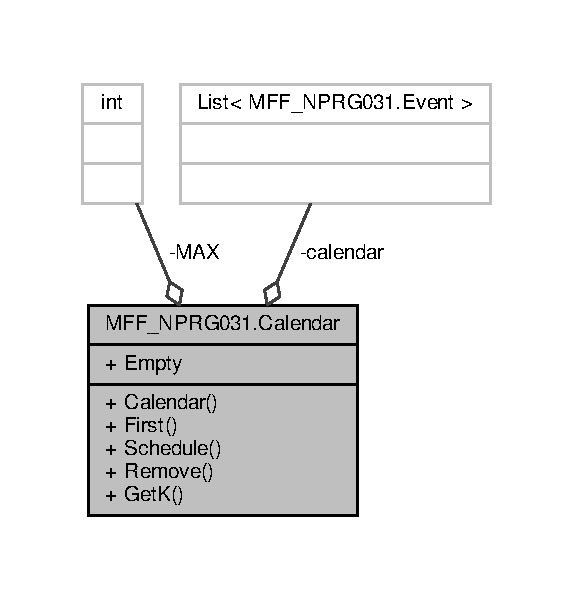
\includegraphics[width=275pt]{classMFF__NPRG031_1_1Calendar__coll__graph}
\end{center}
\end{figure}
\subsection*{Public Member Functions}
\begin{DoxyCompactItemize}
\item 
\hyperlink{classMFF__NPRG031_1_1Calendar_a2279253074472fa30255b2637df30a46}{Calendar} ()
\item 
\hyperlink{classMFF__NPRG031_1_1Event}{Event} \hyperlink{classMFF__NPRG031_1_1Calendar_a623642e4db01cef075845ef5c7db5e0f}{First} ()
\item 
void \hyperlink{classMFF__NPRG031_1_1Calendar_a59c90e97093d8ed21f1c6d36f2a88918}{Schedule} (\hyperlink{classMFF__NPRG031_1_1Event}{Event} e)
\item 
void \hyperlink{classMFF__NPRG031_1_1Calendar_a02ce42eb2c88d16ac1b6296bd9ce7062}{Remove} (\hyperlink{classMFF__NPRG031_1_1Process}{Process} p)
\item 
List$<$ \hyperlink{classMFF__NPRG031_1_1Event}{Event} $>$ \hyperlink{classMFF__NPRG031_1_1Calendar_ab50fb8b653b95205910e61d079ae0676}{Get\-K} ()
\end{DoxyCompactItemize}
\subsection*{Properties}
\begin{DoxyCompactItemize}
\item 
bool \hyperlink{classMFF__NPRG031_1_1Calendar_ac2ebccd4a70e3183e1715ddbde173d06}{Empty}\hspace{0.3cm}{\ttfamily  \mbox{[}get\mbox{]}}
\end{DoxyCompactItemize}
\subsection*{Private Attributes}
\begin{DoxyCompactItemize}
\item 
List$<$ \hyperlink{classMFF__NPRG031_1_1Event}{Event} $>$ \hyperlink{classMFF__NPRG031_1_1Calendar_acaced39a1b5c163830a42abe1c3de960}{calendar} = new List$<$\hyperlink{classMFF__NPRG031_1_1Event}{Event}$>$()
\item 
const int \hyperlink{classMFF__NPRG031_1_1Calendar_a7a57e092fecfd38ee13faa7443704073}{M\-A\-X} = 0x7\-F\-F\-F\-F\-F\-F\-F
\end{DoxyCompactItemize}


\subsection{Constructor \& Destructor Documentation}
\hypertarget{classMFF__NPRG031_1_1Calendar_a2279253074472fa30255b2637df30a46}{\index{M\-F\-F\-\_\-\-N\-P\-R\-G031\-::\-Calendar@{M\-F\-F\-\_\-\-N\-P\-R\-G031\-::\-Calendar}!Calendar@{Calendar}}
\index{Calendar@{Calendar}!MFF_NPRG031::Calendar@{M\-F\-F\-\_\-\-N\-P\-R\-G031\-::\-Calendar}}
\subsubsection[{Calendar}]{\setlength{\rightskip}{0pt plus 5cm}M\-F\-F\-\_\-\-N\-P\-R\-G031.\-Calendar.\-Calendar (
\begin{DoxyParamCaption}
{}
\end{DoxyParamCaption}
)\hspace{0.3cm}{\ttfamily [inline]}}}\label{classMFF__NPRG031_1_1Calendar_a2279253074472fa30255b2637df30a46}


\subsection{Member Function Documentation}
\hypertarget{classMFF__NPRG031_1_1Calendar_a623642e4db01cef075845ef5c7db5e0f}{\index{M\-F\-F\-\_\-\-N\-P\-R\-G031\-::\-Calendar@{M\-F\-F\-\_\-\-N\-P\-R\-G031\-::\-Calendar}!First@{First}}
\index{First@{First}!MFF_NPRG031::Calendar@{M\-F\-F\-\_\-\-N\-P\-R\-G031\-::\-Calendar}}
\subsubsection[{First}]{\setlength{\rightskip}{0pt plus 5cm}{\bf Event} M\-F\-F\-\_\-\-N\-P\-R\-G031.\-Calendar.\-First (
\begin{DoxyParamCaption}
{}
\end{DoxyParamCaption}
)\hspace{0.3cm}{\ttfamily [inline]}}}\label{classMFF__NPRG031_1_1Calendar_a623642e4db01cef075845ef5c7db5e0f}
Returns first event from calendar and removes it from calendar \begin{DoxyReturn}{Returns}
first event from calendar 
\end{DoxyReturn}
\hypertarget{classMFF__NPRG031_1_1Calendar_ab50fb8b653b95205910e61d079ae0676}{\index{M\-F\-F\-\_\-\-N\-P\-R\-G031\-::\-Calendar@{M\-F\-F\-\_\-\-N\-P\-R\-G031\-::\-Calendar}!Get\-K@{Get\-K}}
\index{Get\-K@{Get\-K}!MFF_NPRG031::Calendar@{M\-F\-F\-\_\-\-N\-P\-R\-G031\-::\-Calendar}}
\subsubsection[{Get\-K}]{\setlength{\rightskip}{0pt plus 5cm}List$<${\bf Event}$>$ M\-F\-F\-\_\-\-N\-P\-R\-G031.\-Calendar.\-Get\-K (
\begin{DoxyParamCaption}
{}
\end{DoxyParamCaption}
)\hspace{0.3cm}{\ttfamily [inline]}}}\label{classMFF__NPRG031_1_1Calendar_ab50fb8b653b95205910e61d079ae0676}
Returns inner calendar for testing \begin{DoxyReturn}{Returns}
list of events 
\end{DoxyReturn}
\hypertarget{classMFF__NPRG031_1_1Calendar_a02ce42eb2c88d16ac1b6296bd9ce7062}{\index{M\-F\-F\-\_\-\-N\-P\-R\-G031\-::\-Calendar@{M\-F\-F\-\_\-\-N\-P\-R\-G031\-::\-Calendar}!Remove@{Remove}}
\index{Remove@{Remove}!MFF_NPRG031::Calendar@{M\-F\-F\-\_\-\-N\-P\-R\-G031\-::\-Calendar}}
\subsubsection[{Remove}]{\setlength{\rightskip}{0pt plus 5cm}void M\-F\-F\-\_\-\-N\-P\-R\-G031.\-Calendar.\-Remove (
\begin{DoxyParamCaption}
\item[{{\bf Process}}]{p}
\end{DoxyParamCaption}
)\hspace{0.3cm}{\ttfamily [inline]}}}\label{classMFF__NPRG031_1_1Calendar_a02ce42eb2c88d16ac1b6296bd9ce7062}
Removes process from calendar 
\begin{DoxyParams}{Parameters}
{\em p} & process \\
\hline
\end{DoxyParams}
\hypertarget{classMFF__NPRG031_1_1Calendar_a59c90e97093d8ed21f1c6d36f2a88918}{\index{M\-F\-F\-\_\-\-N\-P\-R\-G031\-::\-Calendar@{M\-F\-F\-\_\-\-N\-P\-R\-G031\-::\-Calendar}!Schedule@{Schedule}}
\index{Schedule@{Schedule}!MFF_NPRG031::Calendar@{M\-F\-F\-\_\-\-N\-P\-R\-G031\-::\-Calendar}}
\subsubsection[{Schedule}]{\setlength{\rightskip}{0pt plus 5cm}void M\-F\-F\-\_\-\-N\-P\-R\-G031.\-Calendar.\-Schedule (
\begin{DoxyParamCaption}
\item[{{\bf Event}}]{e}
\end{DoxyParamCaption}
)\hspace{0.3cm}{\ttfamily [inline]}}}\label{classMFF__NPRG031_1_1Calendar_a59c90e97093d8ed21f1c6d36f2a88918}
Schedules an event by adding it to calendar 
\begin{DoxyParams}{Parameters}
{\em e} & \hyperlink{classMFF__NPRG031_1_1Event}{Event} to schedule \\
\hline
\end{DoxyParams}


\subsection{Member Data Documentation}
\hypertarget{classMFF__NPRG031_1_1Calendar_acaced39a1b5c163830a42abe1c3de960}{\index{M\-F\-F\-\_\-\-N\-P\-R\-G031\-::\-Calendar@{M\-F\-F\-\_\-\-N\-P\-R\-G031\-::\-Calendar}!calendar@{calendar}}
\index{calendar@{calendar}!MFF_NPRG031::Calendar@{M\-F\-F\-\_\-\-N\-P\-R\-G031\-::\-Calendar}}
\subsubsection[{calendar}]{\setlength{\rightskip}{0pt plus 5cm}List$<${\bf Event}$>$ M\-F\-F\-\_\-\-N\-P\-R\-G031.\-Calendar.\-calendar = new List$<${\bf Event}$>$()\hspace{0.3cm}{\ttfamily [private]}}}\label{classMFF__NPRG031_1_1Calendar_acaced39a1b5c163830a42abe1c3de960}
\hypertarget{classMFF__NPRG031_1_1Calendar_a7a57e092fecfd38ee13faa7443704073}{\index{M\-F\-F\-\_\-\-N\-P\-R\-G031\-::\-Calendar@{M\-F\-F\-\_\-\-N\-P\-R\-G031\-::\-Calendar}!M\-A\-X@{M\-A\-X}}
\index{M\-A\-X@{M\-A\-X}!MFF_NPRG031::Calendar@{M\-F\-F\-\_\-\-N\-P\-R\-G031\-::\-Calendar}}
\subsubsection[{M\-A\-X}]{\setlength{\rightskip}{0pt plus 5cm}const int M\-F\-F\-\_\-\-N\-P\-R\-G031.\-Calendar.\-M\-A\-X = 0x7\-F\-F\-F\-F\-F\-F\-F\hspace{0.3cm}{\ttfamily [private]}}}\label{classMFF__NPRG031_1_1Calendar_a7a57e092fecfd38ee13faa7443704073}


\subsection{Property Documentation}
\hypertarget{classMFF__NPRG031_1_1Calendar_ac2ebccd4a70e3183e1715ddbde173d06}{\index{M\-F\-F\-\_\-\-N\-P\-R\-G031\-::\-Calendar@{M\-F\-F\-\_\-\-N\-P\-R\-G031\-::\-Calendar}!Empty@{Empty}}
\index{Empty@{Empty}!MFF_NPRG031::Calendar@{M\-F\-F\-\_\-\-N\-P\-R\-G031\-::\-Calendar}}
\subsubsection[{Empty}]{\setlength{\rightskip}{0pt plus 5cm}bool M\-F\-F\-\_\-\-N\-P\-R\-G031.\-Calendar.\-Empty\hspace{0.3cm}{\ttfamily [get]}}}\label{classMFF__NPRG031_1_1Calendar_ac2ebccd4a70e3183e1715ddbde173d06}
\begin{DoxyReturn}{Returns}
is calendar empty? 
\end{DoxyReturn}


The documentation for this class was generated from the following file\-:\begin{DoxyCompactItemize}
\item 
Net\-Traffic\-Simulator/\-Net\-Traffic\-Simulator/framework/\hyperlink{Calendar_8cs}{Calendar.\-cs}\end{DoxyCompactItemize}

\hypertarget{classNetTrafficSimulator_1_1Link_1_1DataEnvelope}{\section{Net\-Traffic\-Simulator.\-Link.\-Data\-Envelope Class Reference}
\label{classNetTrafficSimulator_1_1Link_1_1DataEnvelope}\index{Net\-Traffic\-Simulator.\-Link.\-Data\-Envelope@{Net\-Traffic\-Simulator.\-Link.\-Data\-Envelope}}
}


Collaboration diagram for Net\-Traffic\-Simulator.\-Link.\-Data\-Envelope\-:\nopagebreak
\begin{figure}[H]
\begin{center}
\leavevmode
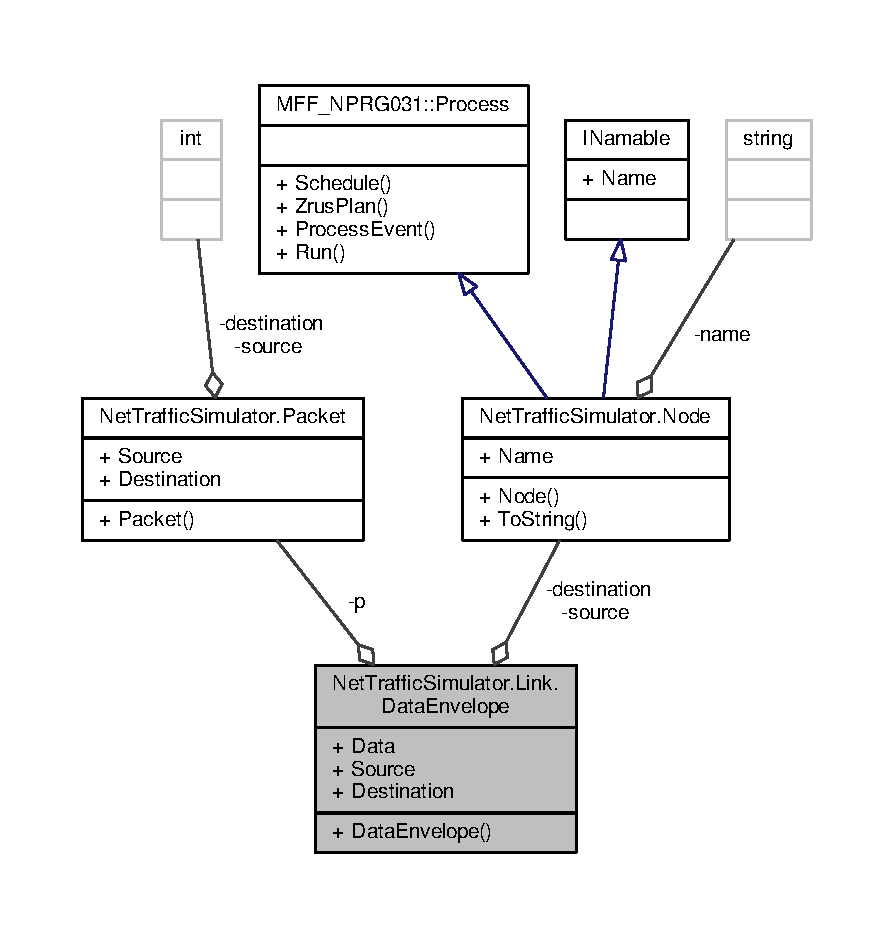
\includegraphics[width=350pt]{classNetTrafficSimulator_1_1Link_1_1DataEnvelope__coll__graph}
\end{center}
\end{figure}
\subsection*{Public Member Functions}
\begin{DoxyCompactItemize}
\item 
\hyperlink{classNetTrafficSimulator_1_1Link_1_1DataEnvelope_aeb2a043396c63e9e27ecce740d877826}{Data\-Envelope} (\hyperlink{classNetTrafficSimulator_1_1Packet}{Packet} \hyperlink{classNetTrafficSimulator_1_1Link_1_1DataEnvelope_a3c8959eec1aeec3d016cc06c5a01a074}{p}, \hyperlink{classNetTrafficSimulator_1_1Node}{Node} \hyperlink{classNetTrafficSimulator_1_1Link_1_1DataEnvelope_a9e56896aa5da48e13e8c13cb9efc20f4}{source}, \hyperlink{classNetTrafficSimulator_1_1Node}{Node} target)
\end{DoxyCompactItemize}
\subsection*{Properties}
\begin{DoxyCompactItemize}
\item 
\hyperlink{classNetTrafficSimulator_1_1Packet}{Packet} \hyperlink{classNetTrafficSimulator_1_1Link_1_1DataEnvelope_ad3d68bcc1cbf160648beeaca939cbd51}{Data}\hspace{0.3cm}{\ttfamily  \mbox{[}get\mbox{]}}
\item 
\hyperlink{classNetTrafficSimulator_1_1Node}{Node} \hyperlink{classNetTrafficSimulator_1_1Link_1_1DataEnvelope_a172d3b86ed384f803eabfa751c4f296f}{Source}\hspace{0.3cm}{\ttfamily  \mbox{[}get\mbox{]}}
\item 
\hyperlink{classNetTrafficSimulator_1_1Node}{Node} \hyperlink{classNetTrafficSimulator_1_1Link_1_1DataEnvelope_af8789d5ec0a0dd7087e33dc532cb0237}{Destination}\hspace{0.3cm}{\ttfamily  \mbox{[}get\mbox{]}}
\end{DoxyCompactItemize}
\subsection*{Private Attributes}
\begin{DoxyCompactItemize}
\item 
\hyperlink{classNetTrafficSimulator_1_1Packet}{Packet} \hyperlink{classNetTrafficSimulator_1_1Link_1_1DataEnvelope_a3c8959eec1aeec3d016cc06c5a01a074}{p}
\item 
\hyperlink{classNetTrafficSimulator_1_1Node}{Node} \hyperlink{classNetTrafficSimulator_1_1Link_1_1DataEnvelope_a9e56896aa5da48e13e8c13cb9efc20f4}{source}
\item 
\hyperlink{classNetTrafficSimulator_1_1Node}{Node} \hyperlink{classNetTrafficSimulator_1_1Link_1_1DataEnvelope_a4c06f49085e916a8e73f54f9c9a148f3}{destination}
\end{DoxyCompactItemize}


\subsection{Constructor \& Destructor Documentation}
\hypertarget{classNetTrafficSimulator_1_1Link_1_1DataEnvelope_aeb2a043396c63e9e27ecce740d877826}{\index{Net\-Traffic\-Simulator\-::\-Link\-::\-Data\-Envelope@{Net\-Traffic\-Simulator\-::\-Link\-::\-Data\-Envelope}!Data\-Envelope@{Data\-Envelope}}
\index{Data\-Envelope@{Data\-Envelope}!NetTrafficSimulator::Link::DataEnvelope@{Net\-Traffic\-Simulator\-::\-Link\-::\-Data\-Envelope}}
\subsubsection[{Data\-Envelope}]{\setlength{\rightskip}{0pt plus 5cm}Net\-Traffic\-Simulator.\-Link.\-Data\-Envelope.\-Data\-Envelope (
\begin{DoxyParamCaption}
\item[{{\bf Packet}}]{p, }
\item[{{\bf Node}}]{source, }
\item[{{\bf Node}}]{target}
\end{DoxyParamCaption}
)\hspace{0.3cm}{\ttfamily [inline]}}}\label{classNetTrafficSimulator_1_1Link_1_1DataEnvelope_aeb2a043396c63e9e27ecce740d877826}
Create a \hyperlink{classNetTrafficSimulator_1_1Link_1_1DataEnvelope}{Data\-Envelope} given the packet, source and target \hyperlink{classNetTrafficSimulator_1_1Link_1_1DataEnvelope}{Data\-Envelope} specifies direction of data flow since link is full duplex 
\begin{DoxyParams}{Parameters}
{\em p} & \hyperlink{classNetTrafficSimulator_1_1Packet}{Packet} to deliver \\
\hline
{\em source} & \hyperlink{classNetTrafficSimulator_1_1Packet}{Packet} sender \\
\hline
{\em target} & \hyperlink{classNetTrafficSimulator_1_1Packet}{Packet} receiver \\
\hline
\end{DoxyParams}


\subsection{Member Data Documentation}
\hypertarget{classNetTrafficSimulator_1_1Link_1_1DataEnvelope_a4c06f49085e916a8e73f54f9c9a148f3}{\index{Net\-Traffic\-Simulator\-::\-Link\-::\-Data\-Envelope@{Net\-Traffic\-Simulator\-::\-Link\-::\-Data\-Envelope}!destination@{destination}}
\index{destination@{destination}!NetTrafficSimulator::Link::DataEnvelope@{Net\-Traffic\-Simulator\-::\-Link\-::\-Data\-Envelope}}
\subsubsection[{destination}]{\setlength{\rightskip}{0pt plus 5cm}{\bf Node} Net\-Traffic\-Simulator.\-Link.\-Data\-Envelope.\-destination\hspace{0.3cm}{\ttfamily [private]}}}\label{classNetTrafficSimulator_1_1Link_1_1DataEnvelope_a4c06f49085e916a8e73f54f9c9a148f3}
\hypertarget{classNetTrafficSimulator_1_1Link_1_1DataEnvelope_a3c8959eec1aeec3d016cc06c5a01a074}{\index{Net\-Traffic\-Simulator\-::\-Link\-::\-Data\-Envelope@{Net\-Traffic\-Simulator\-::\-Link\-::\-Data\-Envelope}!p@{p}}
\index{p@{p}!NetTrafficSimulator::Link::DataEnvelope@{Net\-Traffic\-Simulator\-::\-Link\-::\-Data\-Envelope}}
\subsubsection[{p}]{\setlength{\rightskip}{0pt plus 5cm}{\bf Packet} Net\-Traffic\-Simulator.\-Link.\-Data\-Envelope.\-p\hspace{0.3cm}{\ttfamily [private]}}}\label{classNetTrafficSimulator_1_1Link_1_1DataEnvelope_a3c8959eec1aeec3d016cc06c5a01a074}
\hypertarget{classNetTrafficSimulator_1_1Link_1_1DataEnvelope_a9e56896aa5da48e13e8c13cb9efc20f4}{\index{Net\-Traffic\-Simulator\-::\-Link\-::\-Data\-Envelope@{Net\-Traffic\-Simulator\-::\-Link\-::\-Data\-Envelope}!source@{source}}
\index{source@{source}!NetTrafficSimulator::Link::DataEnvelope@{Net\-Traffic\-Simulator\-::\-Link\-::\-Data\-Envelope}}
\subsubsection[{source}]{\setlength{\rightskip}{0pt plus 5cm}{\bf Node} Net\-Traffic\-Simulator.\-Link.\-Data\-Envelope.\-source\hspace{0.3cm}{\ttfamily [private]}}}\label{classNetTrafficSimulator_1_1Link_1_1DataEnvelope_a9e56896aa5da48e13e8c13cb9efc20f4}


\subsection{Property Documentation}
\hypertarget{classNetTrafficSimulator_1_1Link_1_1DataEnvelope_ad3d68bcc1cbf160648beeaca939cbd51}{\index{Net\-Traffic\-Simulator\-::\-Link\-::\-Data\-Envelope@{Net\-Traffic\-Simulator\-::\-Link\-::\-Data\-Envelope}!Data@{Data}}
\index{Data@{Data}!NetTrafficSimulator::Link::DataEnvelope@{Net\-Traffic\-Simulator\-::\-Link\-::\-Data\-Envelope}}
\subsubsection[{Data}]{\setlength{\rightskip}{0pt plus 5cm}{\bf Packet} Net\-Traffic\-Simulator.\-Link.\-Data\-Envelope.\-Data\hspace{0.3cm}{\ttfamily [get]}}}\label{classNetTrafficSimulator_1_1Link_1_1DataEnvelope_ad3d68bcc1cbf160648beeaca939cbd51}
The packet \hypertarget{classNetTrafficSimulator_1_1Link_1_1DataEnvelope_af8789d5ec0a0dd7087e33dc532cb0237}{\index{Net\-Traffic\-Simulator\-::\-Link\-::\-Data\-Envelope@{Net\-Traffic\-Simulator\-::\-Link\-::\-Data\-Envelope}!Destination@{Destination}}
\index{Destination@{Destination}!NetTrafficSimulator::Link::DataEnvelope@{Net\-Traffic\-Simulator\-::\-Link\-::\-Data\-Envelope}}
\subsubsection[{Destination}]{\setlength{\rightskip}{0pt plus 5cm}{\bf Node} Net\-Traffic\-Simulator.\-Link.\-Data\-Envelope.\-Destination\hspace{0.3cm}{\ttfamily [get]}}}\label{classNetTrafficSimulator_1_1Link_1_1DataEnvelope_af8789d5ec0a0dd7087e33dc532cb0237}
The receiver \hypertarget{classNetTrafficSimulator_1_1Link_1_1DataEnvelope_a172d3b86ed384f803eabfa751c4f296f}{\index{Net\-Traffic\-Simulator\-::\-Link\-::\-Data\-Envelope@{Net\-Traffic\-Simulator\-::\-Link\-::\-Data\-Envelope}!Source@{Source}}
\index{Source@{Source}!NetTrafficSimulator::Link::DataEnvelope@{Net\-Traffic\-Simulator\-::\-Link\-::\-Data\-Envelope}}
\subsubsection[{Source}]{\setlength{\rightskip}{0pt plus 5cm}{\bf Node} Net\-Traffic\-Simulator.\-Link.\-Data\-Envelope.\-Source\hspace{0.3cm}{\ttfamily [get]}}}\label{classNetTrafficSimulator_1_1Link_1_1DataEnvelope_a172d3b86ed384f803eabfa751c4f296f}
The sender 

The documentation for this class was generated from the following file\-:\begin{DoxyCompactItemize}
\item 
Net\-Traffic\-Simulator/\-Net\-Traffic\-Simulator/framework/extension/\hyperlink{Link_8cs}{Link.\-cs}\end{DoxyCompactItemize}

\hypertarget{classNetTrafficSimulator_1_1EndNode}{\section{Net\-Traffic\-Simulator.\-End\-Node Class Reference}
\label{classNetTrafficSimulator_1_1EndNode}\index{Net\-Traffic\-Simulator.\-End\-Node@{Net\-Traffic\-Simulator.\-End\-Node}}
}


Inheritance diagram for Net\-Traffic\-Simulator.\-End\-Node\-:
\nopagebreak
\begin{figure}[H]
\begin{center}
\leavevmode
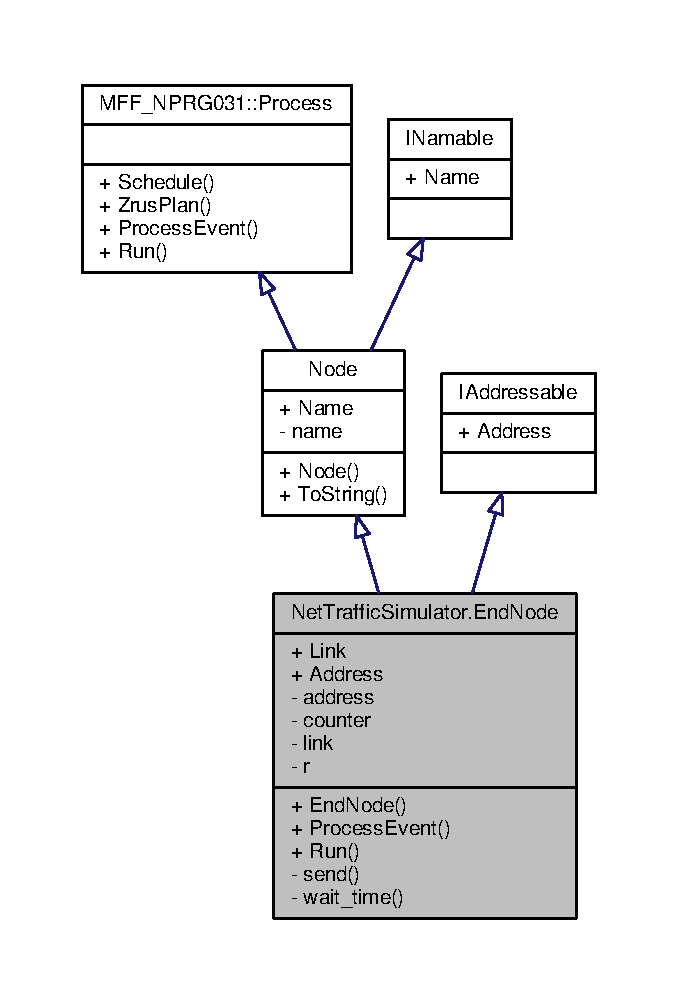
\includegraphics[width=350pt]{classNetTrafficSimulator_1_1EndNode__inherit__graph}
\end{center}
\end{figure}


Collaboration diagram for Net\-Traffic\-Simulator.\-End\-Node\-:
\nopagebreak
\begin{figure}[H]
\begin{center}
\leavevmode
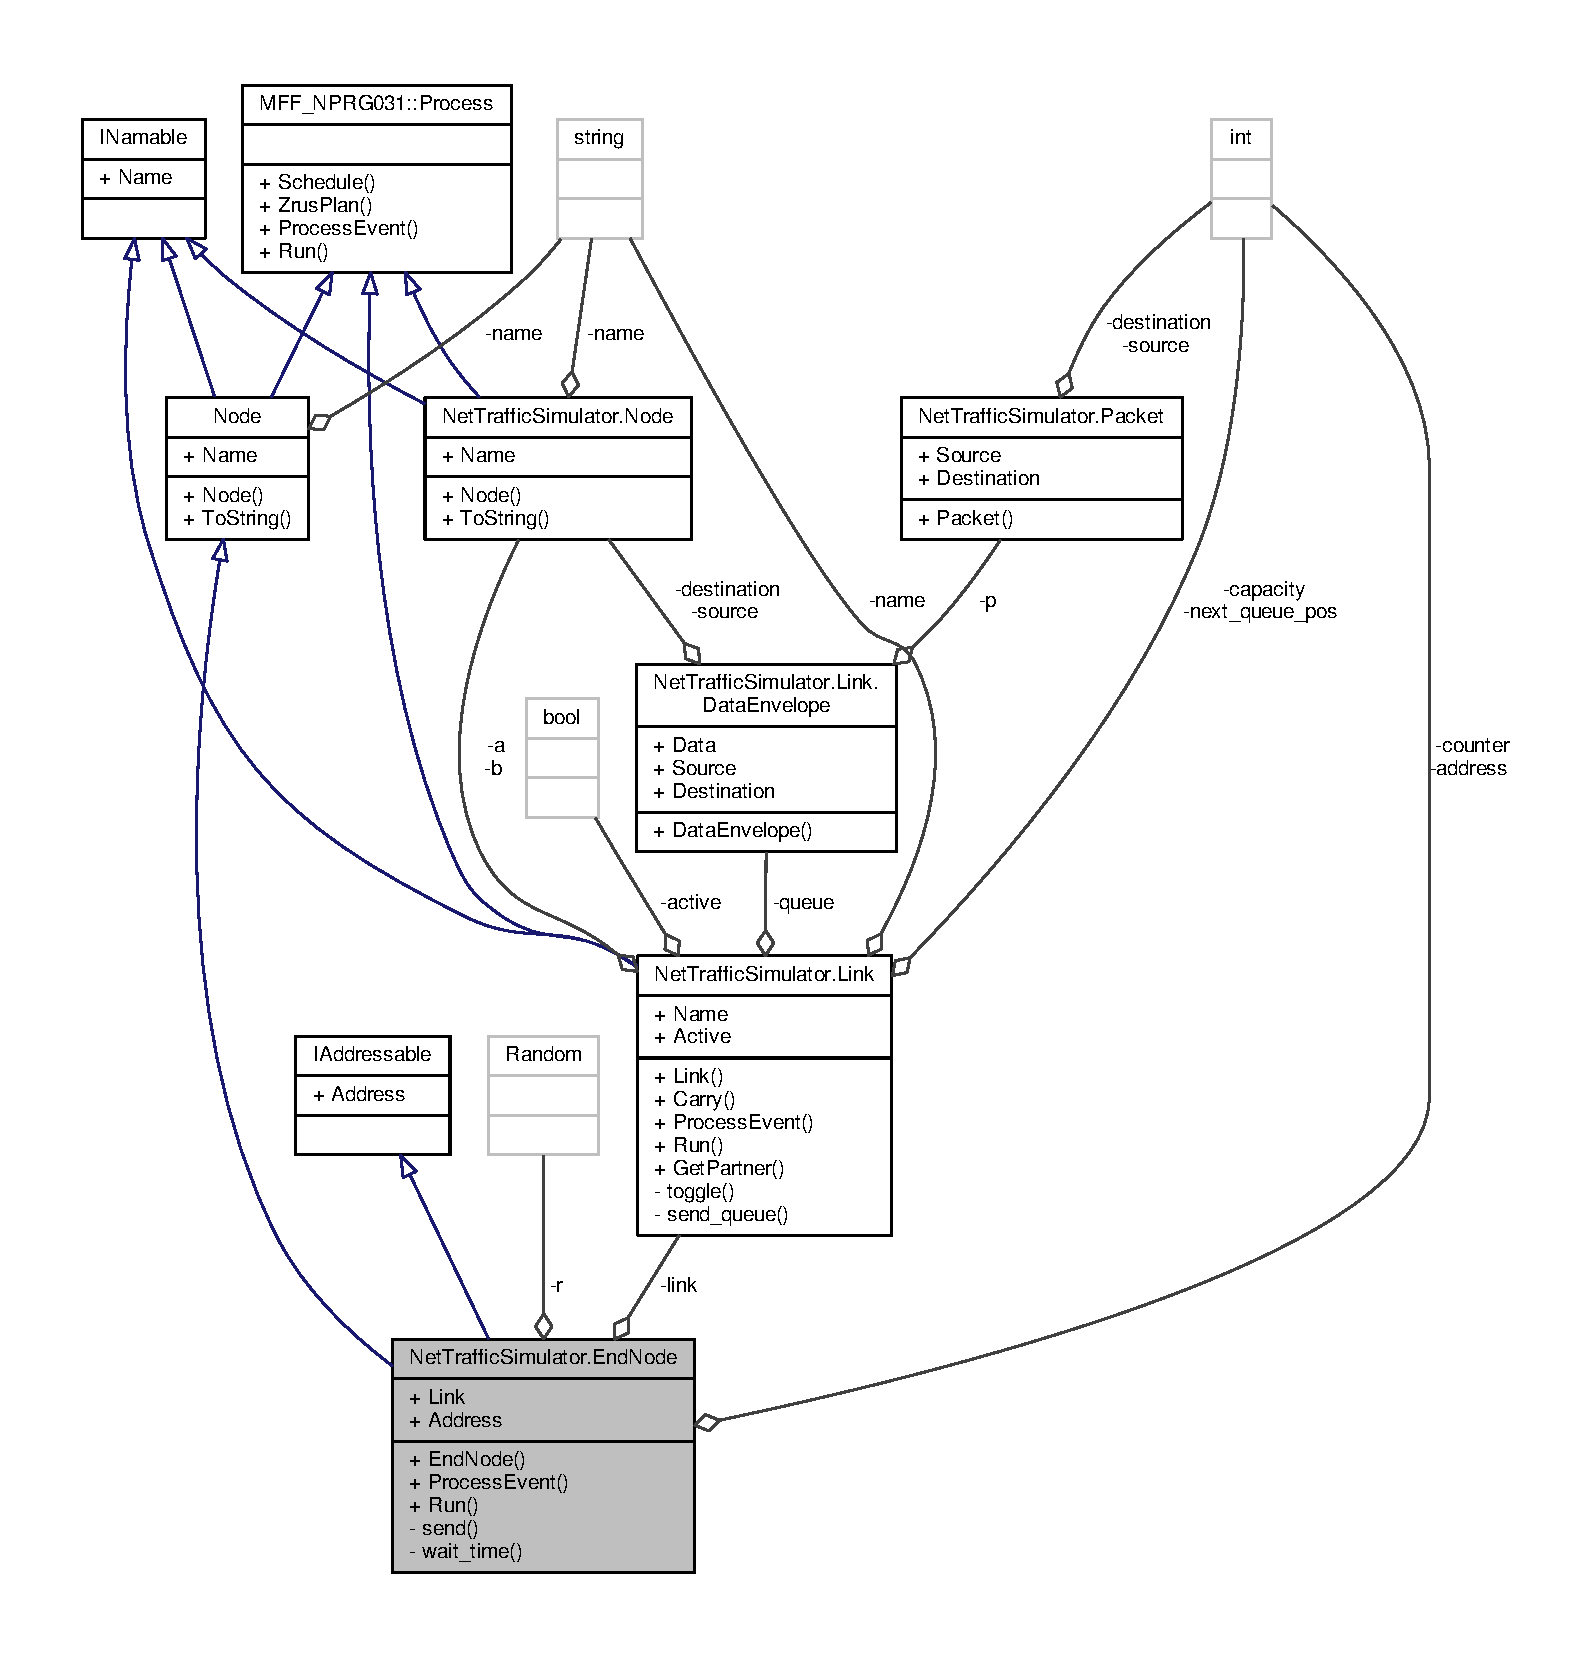
\includegraphics[width=350pt]{classNetTrafficSimulator_1_1EndNode__coll__graph}
\end{center}
\end{figure}
\subsection*{Public Member Functions}
\begin{DoxyCompactItemize}
\item 
\hyperlink{classNetTrafficSimulator_1_1EndNode_ab690976d2c39fafef1f5e5ad0a708ee8}{End\-Node} (String n, int \hyperlink{classNetTrafficSimulator_1_1EndNode_a84d0df6c9c755c895dffff6a531823d2}{address})
\item 
override void \hyperlink{classNetTrafficSimulator_1_1EndNode_a54624ab4b68ccc8c938905ac3e906623}{Process\-Event} (\hyperlink{classMFF__NPRG031_1_1State}{M\-F\-F\-\_\-\-N\-P\-R\-G031.\-State} state, \hyperlink{classMFF__NPRG031_1_1Model}{M\-F\-F\-\_\-\-N\-P\-R\-G031.\-Model} model)
\item 
override void \hyperlink{classNetTrafficSimulator_1_1EndNode_ad672744610489948d0a8126a84a1aab6}{Run} (\hyperlink{classMFF__NPRG031_1_1Model}{M\-F\-F\-\_\-\-N\-P\-R\-G031.\-Model} m)
\item 
Dictionary$<$ string, object $>$ \hyperlink{classNetTrafficSimulator_1_1EndNode_aade90e936fa0903c728fc484be8a57d2}{Get\-Results} (\hyperlink{classMFF__NPRG031_1_1Model}{M\-F\-F\-\_\-\-N\-P\-R\-G031.\-Model} model)
\end{DoxyCompactItemize}
\subsection*{Properties}
\begin{DoxyCompactItemize}
\item 
\hyperlink{classNetTrafficSimulator_1_1Link}{Link} \hyperlink{classNetTrafficSimulator_1_1EndNode_aaa7c476166fa515ebc9d16c6ccc83875}{Link}\hspace{0.3cm}{\ttfamily  \mbox{[}get, set\mbox{]}}
\item 
int \hyperlink{classNetTrafficSimulator_1_1EndNode_ad810757c44c8e17c2147a2ae1598a840}{Address}\hspace{0.3cm}{\ttfamily  \mbox{[}get\mbox{]}}
\end{DoxyCompactItemize}
\subsection*{Private Member Functions}
\begin{DoxyCompactItemize}
\item 
void \hyperlink{classNetTrafficSimulator_1_1EndNode_a021bef61770e7ec3561b24edca6526ba}{send} ()
\item 
int \hyperlink{classNetTrafficSimulator_1_1EndNode_a9287a628dea98e2611bde679eb3c63da}{wait\-\_\-time} ()
\end{DoxyCompactItemize}
\subsection*{Private Attributes}
\begin{DoxyCompactItemize}
\item 
readonly int \hyperlink{classNetTrafficSimulator_1_1EndNode_a84d0df6c9c755c895dffff6a531823d2}{address}
\item 
int \hyperlink{classNetTrafficSimulator_1_1EndNode_a45bd4418f00eb56fde0618470a05688e}{sent}
\item 
int \hyperlink{classNetTrafficSimulator_1_1EndNode_aec9de5a4499a35773abb2e5ebc6b153e}{received}
\item 
int \hyperlink{classNetTrafficSimulator_1_1EndNode_a92b73535be26c46a619a2c307ecd3ad4}{time\-\_\-wait}
\item 
\hyperlink{classNetTrafficSimulator_1_1Link}{Link} \hyperlink{classNetTrafficSimulator_1_1EndNode_a3fde207ff4a49bafd01df2e89fff7d11}{link}
\item 
Random \hyperlink{classNetTrafficSimulator_1_1EndNode_ab68702887e7cdb3933a3a006ea508a76}{r}
\end{DoxyCompactItemize}


\subsection{Constructor \& Destructor Documentation}
\hypertarget{classNetTrafficSimulator_1_1EndNode_ab690976d2c39fafef1f5e5ad0a708ee8}{\index{Net\-Traffic\-Simulator\-::\-End\-Node@{Net\-Traffic\-Simulator\-::\-End\-Node}!End\-Node@{End\-Node}}
\index{End\-Node@{End\-Node}!NetTrafficSimulator::EndNode@{Net\-Traffic\-Simulator\-::\-End\-Node}}
\subsubsection[{End\-Node}]{\setlength{\rightskip}{0pt plus 5cm}Net\-Traffic\-Simulator.\-End\-Node.\-End\-Node (
\begin{DoxyParamCaption}
\item[{String}]{n, }
\item[{int}]{address}
\end{DoxyParamCaption}
)\hspace{0.3cm}{\ttfamily [inline]}}}\label{classNetTrafficSimulator_1_1EndNode_ab690976d2c39fafef1f5e5ad0a708ee8}
Creates an \hyperlink{classNetTrafficSimulator_1_1EndNode}{End\-Node} with given name and address 

\subsection{Member Function Documentation}
\hypertarget{classNetTrafficSimulator_1_1EndNode_aade90e936fa0903c728fc484be8a57d2}{\index{Net\-Traffic\-Simulator\-::\-End\-Node@{Net\-Traffic\-Simulator\-::\-End\-Node}!Get\-Results@{Get\-Results}}
\index{Get\-Results@{Get\-Results}!NetTrafficSimulator::EndNode@{Net\-Traffic\-Simulator\-::\-End\-Node}}
\subsubsection[{Get\-Results}]{\setlength{\rightskip}{0pt plus 5cm}Dictionary$<$string,object$>$ Net\-Traffic\-Simulator.\-End\-Node.\-Get\-Results (
\begin{DoxyParamCaption}
\item[{{\bf M\-F\-F\-\_\-\-N\-P\-R\-G031.\-Model}}]{model}
\end{DoxyParamCaption}
)\hspace{0.3cm}{\ttfamily [inline]}}}\label{classNetTrafficSimulator_1_1EndNode_aade90e936fa0903c728fc484be8a57d2}
Provide results measured during simulation for populating a result model \begin{DoxyReturn}{Returns}
Dictionary, where string is a key representing a human-\/readable description of measured data and object is value measured 
\end{DoxyReturn}


Implements \hyperlink{interfaceNetTrafficSimulator_1_1IResultProvider_ac7053c11f509ba1c2f653cd952b05323}{Net\-Traffic\-Simulator.\-I\-Result\-Provider}.

\hypertarget{classNetTrafficSimulator_1_1EndNode_a54624ab4b68ccc8c938905ac3e906623}{\index{Net\-Traffic\-Simulator\-::\-End\-Node@{Net\-Traffic\-Simulator\-::\-End\-Node}!Process\-Event@{Process\-Event}}
\index{Process\-Event@{Process\-Event}!NetTrafficSimulator::EndNode@{Net\-Traffic\-Simulator\-::\-End\-Node}}
\subsubsection[{Process\-Event}]{\setlength{\rightskip}{0pt plus 5cm}override void Net\-Traffic\-Simulator.\-End\-Node.\-Process\-Event (
\begin{DoxyParamCaption}
\item[{{\bf M\-F\-F\-\_\-\-N\-P\-R\-G031.\-State}}]{state, }
\item[{{\bf M\-F\-F\-\_\-\-N\-P\-R\-G031.\-Model}}]{model}
\end{DoxyParamCaption}
)\hspace{0.3cm}{\ttfamily [inline]}, {\ttfamily [virtual]}}}\label{classNetTrafficSimulator_1_1EndNode_a54624ab4b68ccc8c938905ac3e906623}
Abstract method Process\-Event for process to react on event hapened 
\begin{DoxyParams}{Parameters}
{\em state} & In what state the process is now \\
\hline
{\em model} & Our simulation model \\
\hline
\end{DoxyParams}


Implements \hyperlink{classMFF__NPRG031_1_1Process_acb58d206e76c177264614d88f1818fdc}{M\-F\-F\-\_\-\-N\-P\-R\-G031.\-Process}.



Here is the call graph for this function\-:\nopagebreak
\begin{figure}[H]
\begin{center}
\leavevmode
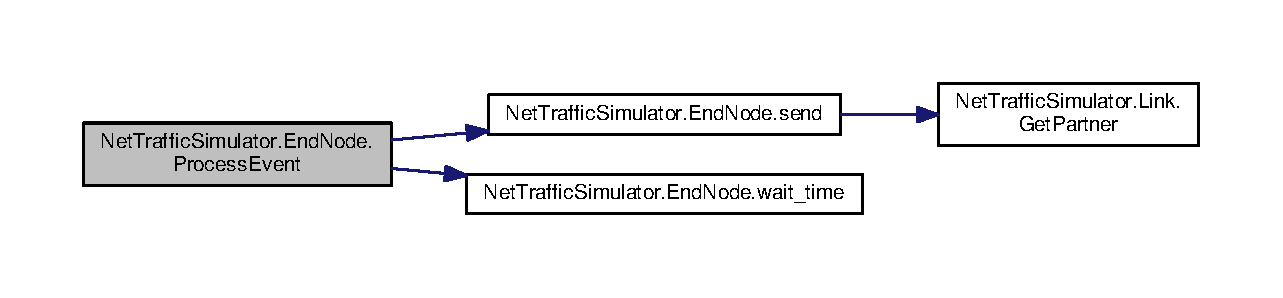
\includegraphics[width=350pt]{classNetTrafficSimulator_1_1EndNode_a54624ab4b68ccc8c938905ac3e906623_cgraph}
\end{center}
\end{figure}


\hypertarget{classNetTrafficSimulator_1_1EndNode_ad672744610489948d0a8126a84a1aab6}{\index{Net\-Traffic\-Simulator\-::\-End\-Node@{Net\-Traffic\-Simulator\-::\-End\-Node}!Run@{Run}}
\index{Run@{Run}!NetTrafficSimulator::EndNode@{Net\-Traffic\-Simulator\-::\-End\-Node}}
\subsubsection[{Run}]{\setlength{\rightskip}{0pt plus 5cm}override void Net\-Traffic\-Simulator.\-End\-Node.\-Run (
\begin{DoxyParamCaption}
\item[{{\bf M\-F\-F\-\_\-\-N\-P\-R\-G031.\-Model}}]{m}
\end{DoxyParamCaption}
)\hspace{0.3cm}{\ttfamily [inline]}, {\ttfamily [virtual]}}}\label{classNetTrafficSimulator_1_1EndNode_ad672744610489948d0a8126a84a1aab6}
Initial set up 
\begin{DoxyParams}{Parameters}
{\em m} & Model given \\
\hline
\end{DoxyParams}


Implements \hyperlink{classMFF__NPRG031_1_1Process_ad0e440dee98ba26c59ab22a60ebcafdd}{M\-F\-F\-\_\-\-N\-P\-R\-G031.\-Process}.

\hypertarget{classNetTrafficSimulator_1_1EndNode_a021bef61770e7ec3561b24edca6526ba}{\index{Net\-Traffic\-Simulator\-::\-End\-Node@{Net\-Traffic\-Simulator\-::\-End\-Node}!send@{send}}
\index{send@{send}!NetTrafficSimulator::EndNode@{Net\-Traffic\-Simulator\-::\-End\-Node}}
\subsubsection[{send}]{\setlength{\rightskip}{0pt plus 5cm}void Net\-Traffic\-Simulator.\-End\-Node.\-send (
\begin{DoxyParamCaption}
{}
\end{DoxyParamCaption}
)\hspace{0.3cm}{\ttfamily [inline]}, {\ttfamily [private]}}}\label{classNetTrafficSimulator_1_1EndNode_a021bef61770e7ec3561b24edca6526ba}
Attept to post a new packet to the link, if such exist 
\begin{DoxyExceptions}{Exceptions}
{\em Invalid\-Operation\-Exception} & if link is not connected \\
\hline
\end{DoxyExceptions}


Here is the call graph for this function\-:\nopagebreak
\begin{figure}[H]
\begin{center}
\leavevmode
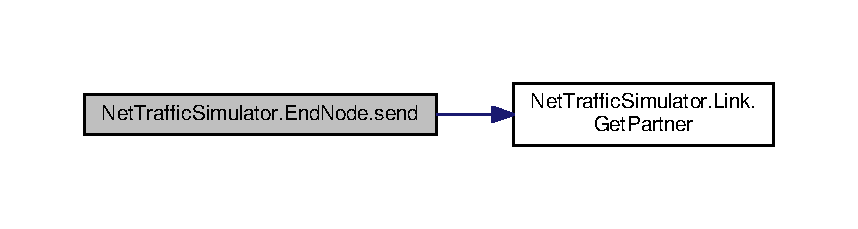
\includegraphics[width=350pt]{classNetTrafficSimulator_1_1EndNode_a021bef61770e7ec3561b24edca6526ba_cgraph}
\end{center}
\end{figure}




Here is the caller graph for this function\-:\nopagebreak
\begin{figure}[H]
\begin{center}
\leavevmode
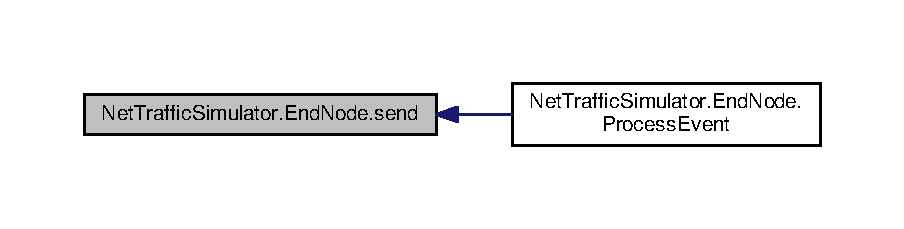
\includegraphics[width=350pt]{classNetTrafficSimulator_1_1EndNode_a021bef61770e7ec3561b24edca6526ba_icgraph}
\end{center}
\end{figure}


\hypertarget{classNetTrafficSimulator_1_1EndNode_a9287a628dea98e2611bde679eb3c63da}{\index{Net\-Traffic\-Simulator\-::\-End\-Node@{Net\-Traffic\-Simulator\-::\-End\-Node}!wait\-\_\-time@{wait\-\_\-time}}
\index{wait\-\_\-time@{wait\-\_\-time}!NetTrafficSimulator::EndNode@{Net\-Traffic\-Simulator\-::\-End\-Node}}
\subsubsection[{wait\-\_\-time}]{\setlength{\rightskip}{0pt plus 5cm}int Net\-Traffic\-Simulator.\-End\-Node.\-wait\-\_\-time (
\begin{DoxyParamCaption}
{}
\end{DoxyParamCaption}
)\hspace{0.3cm}{\ttfamily [inline]}, {\ttfamily [private]}}}\label{classNetTrafficSimulator_1_1EndNode_a9287a628dea98e2611bde679eb3c63da}
Generates a wait time after sending 

Here is the caller graph for this function\-:\nopagebreak
\begin{figure}[H]
\begin{center}
\leavevmode
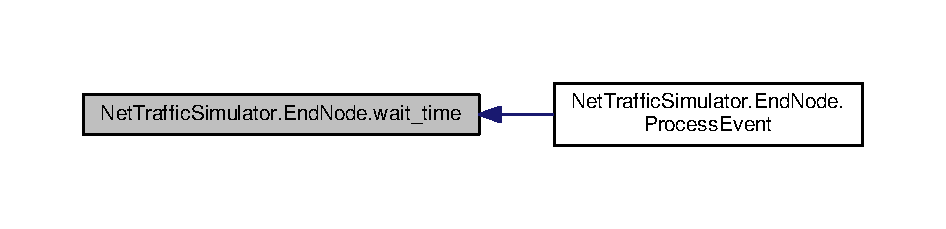
\includegraphics[width=350pt]{classNetTrafficSimulator_1_1EndNode_a9287a628dea98e2611bde679eb3c63da_icgraph}
\end{center}
\end{figure}




\subsection{Member Data Documentation}
\hypertarget{classNetTrafficSimulator_1_1EndNode_a84d0df6c9c755c895dffff6a531823d2}{\index{Net\-Traffic\-Simulator\-::\-End\-Node@{Net\-Traffic\-Simulator\-::\-End\-Node}!address@{address}}
\index{address@{address}!NetTrafficSimulator::EndNode@{Net\-Traffic\-Simulator\-::\-End\-Node}}
\subsubsection[{address}]{\setlength{\rightskip}{0pt plus 5cm}readonly int Net\-Traffic\-Simulator.\-End\-Node.\-address\hspace{0.3cm}{\ttfamily [private]}}}\label{classNetTrafficSimulator_1_1EndNode_a84d0df6c9c755c895dffff6a531823d2}
\hypertarget{classNetTrafficSimulator_1_1EndNode_a3fde207ff4a49bafd01df2e89fff7d11}{\index{Net\-Traffic\-Simulator\-::\-End\-Node@{Net\-Traffic\-Simulator\-::\-End\-Node}!link@{link}}
\index{link@{link}!NetTrafficSimulator::EndNode@{Net\-Traffic\-Simulator\-::\-End\-Node}}
\subsubsection[{link}]{\setlength{\rightskip}{0pt plus 5cm}{\bf Link} Net\-Traffic\-Simulator.\-End\-Node.\-link\hspace{0.3cm}{\ttfamily [private]}}}\label{classNetTrafficSimulator_1_1EndNode_a3fde207ff4a49bafd01df2e89fff7d11}
\hypertarget{classNetTrafficSimulator_1_1EndNode_ab68702887e7cdb3933a3a006ea508a76}{\index{Net\-Traffic\-Simulator\-::\-End\-Node@{Net\-Traffic\-Simulator\-::\-End\-Node}!r@{r}}
\index{r@{r}!NetTrafficSimulator::EndNode@{Net\-Traffic\-Simulator\-::\-End\-Node}}
\subsubsection[{r}]{\setlength{\rightskip}{0pt plus 5cm}Random Net\-Traffic\-Simulator.\-End\-Node.\-r\hspace{0.3cm}{\ttfamily [private]}}}\label{classNetTrafficSimulator_1_1EndNode_ab68702887e7cdb3933a3a006ea508a76}
\hypertarget{classNetTrafficSimulator_1_1EndNode_aec9de5a4499a35773abb2e5ebc6b153e}{\index{Net\-Traffic\-Simulator\-::\-End\-Node@{Net\-Traffic\-Simulator\-::\-End\-Node}!received@{received}}
\index{received@{received}!NetTrafficSimulator::EndNode@{Net\-Traffic\-Simulator\-::\-End\-Node}}
\subsubsection[{received}]{\setlength{\rightskip}{0pt plus 5cm}int Net\-Traffic\-Simulator.\-End\-Node.\-received\hspace{0.3cm}{\ttfamily [private]}}}\label{classNetTrafficSimulator_1_1EndNode_aec9de5a4499a35773abb2e5ebc6b153e}
\hypertarget{classNetTrafficSimulator_1_1EndNode_a45bd4418f00eb56fde0618470a05688e}{\index{Net\-Traffic\-Simulator\-::\-End\-Node@{Net\-Traffic\-Simulator\-::\-End\-Node}!sent@{sent}}
\index{sent@{sent}!NetTrafficSimulator::EndNode@{Net\-Traffic\-Simulator\-::\-End\-Node}}
\subsubsection[{sent}]{\setlength{\rightskip}{0pt plus 5cm}int Net\-Traffic\-Simulator.\-End\-Node.\-sent\hspace{0.3cm}{\ttfamily [private]}}}\label{classNetTrafficSimulator_1_1EndNode_a45bd4418f00eb56fde0618470a05688e}
\hypertarget{classNetTrafficSimulator_1_1EndNode_a92b73535be26c46a619a2c307ecd3ad4}{\index{Net\-Traffic\-Simulator\-::\-End\-Node@{Net\-Traffic\-Simulator\-::\-End\-Node}!time\-\_\-wait@{time\-\_\-wait}}
\index{time\-\_\-wait@{time\-\_\-wait}!NetTrafficSimulator::EndNode@{Net\-Traffic\-Simulator\-::\-End\-Node}}
\subsubsection[{time\-\_\-wait}]{\setlength{\rightskip}{0pt plus 5cm}int Net\-Traffic\-Simulator.\-End\-Node.\-time\-\_\-wait\hspace{0.3cm}{\ttfamily [private]}}}\label{classNetTrafficSimulator_1_1EndNode_a92b73535be26c46a619a2c307ecd3ad4}


\subsection{Property Documentation}
\hypertarget{classNetTrafficSimulator_1_1EndNode_ad810757c44c8e17c2147a2ae1598a840}{\index{Net\-Traffic\-Simulator\-::\-End\-Node@{Net\-Traffic\-Simulator\-::\-End\-Node}!Address@{Address}}
\index{Address@{Address}!NetTrafficSimulator::EndNode@{Net\-Traffic\-Simulator\-::\-End\-Node}}
\subsubsection[{Address}]{\setlength{\rightskip}{0pt plus 5cm}int Net\-Traffic\-Simulator.\-End\-Node.\-Address\hspace{0.3cm}{\ttfamily [get]}}}\label{classNetTrafficSimulator_1_1EndNode_ad810757c44c8e17c2147a2ae1598a840}
Network address of the node \hypertarget{classNetTrafficSimulator_1_1EndNode_aaa7c476166fa515ebc9d16c6ccc83875}{\index{Net\-Traffic\-Simulator\-::\-End\-Node@{Net\-Traffic\-Simulator\-::\-End\-Node}!Link@{Link}}
\index{Link@{Link}!NetTrafficSimulator::EndNode@{Net\-Traffic\-Simulator\-::\-End\-Node}}
\subsubsection[{Link}]{\setlength{\rightskip}{0pt plus 5cm}{\bf Link} Net\-Traffic\-Simulator.\-End\-Node.\-Link\hspace{0.3cm}{\ttfamily [get]}, {\ttfamily [set]}}}\label{classNetTrafficSimulator_1_1EndNode_aaa7c476166fa515ebc9d16c6ccc83875}
\hyperlink{classNetTrafficSimulator_1_1Link}{Link} connecting the \hyperlink{classNetTrafficSimulator_1_1EndNode}{End\-Node} to the rest of the network 

The documentation for this class was generated from the following file\-:\begin{DoxyCompactItemize}
\item 
Net\-Traffic\-Simulator/\-Net\-Traffic\-Simulator/framework/extension/\hyperlink{EndNode_8cs}{End\-Node.\-cs}\end{DoxyCompactItemize}

\hypertarget{classMFF__NPRG031_1_1Event}{\section{M\-F\-F\-\_\-\-N\-P\-R\-G031.\-Event Class Reference}
\label{classMFF__NPRG031_1_1Event}\index{M\-F\-F\-\_\-\-N\-P\-R\-G031.\-Event@{M\-F\-F\-\_\-\-N\-P\-R\-G031.\-Event}}
}


Collaboration diagram for M\-F\-F\-\_\-\-N\-P\-R\-G031.\-Event\-:\nopagebreak
\begin{figure}[H]
\begin{center}
\leavevmode
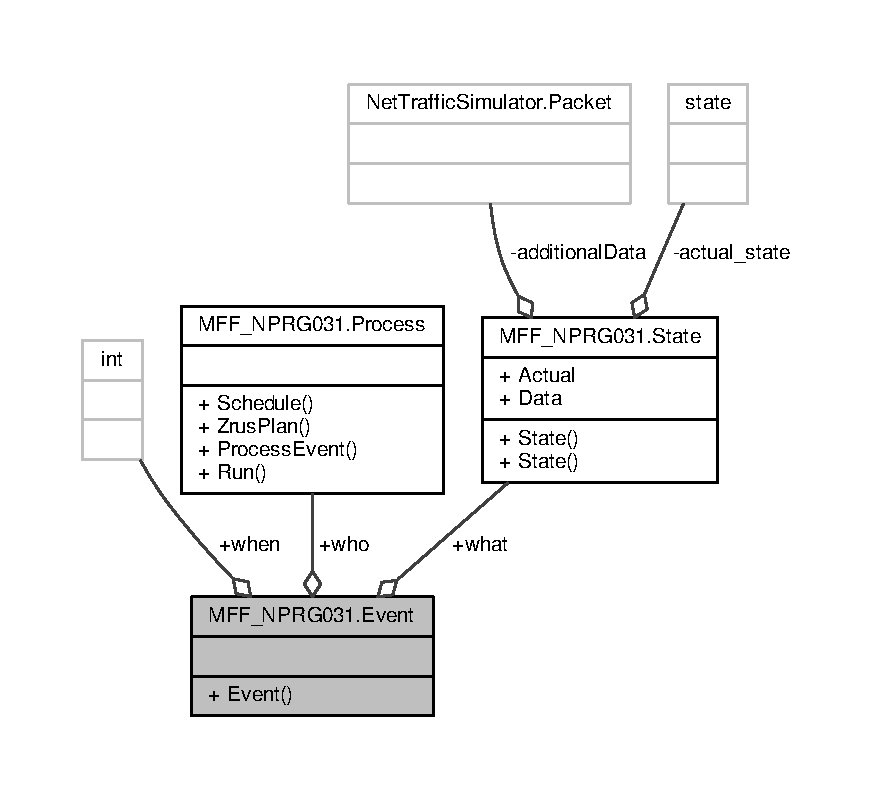
\includegraphics[width=350pt]{classMFF__NPRG031_1_1Event__coll__graph}
\end{center}
\end{figure}
\subsection*{Public Member Functions}
\begin{DoxyCompactItemize}
\item 
\hyperlink{classMFF__NPRG031_1_1Event_adbd83e9064636ea352f06fb82fc2fb29}{Event} (\hyperlink{classMFF__NPRG031_1_1Process}{Process} \hyperlink{classMFF__NPRG031_1_1Event_a6e7bdfc2ff5a26bd896029b56d8f0756}{who}, \hyperlink{classMFF__NPRG031_1_1State}{State} \hyperlink{classMFF__NPRG031_1_1Event_a67299cb9ed36b10f47f75d41a270b4b7}{what}, int \hyperlink{classMFF__NPRG031_1_1Event_a7a80c569961ddf9f12ef8f7cb5782794}{when})
\end{DoxyCompactItemize}
\subsection*{Public Attributes}
\begin{DoxyCompactItemize}
\item 
\hyperlink{classMFF__NPRG031_1_1Process}{Process} \hyperlink{classMFF__NPRG031_1_1Event_a6e7bdfc2ff5a26bd896029b56d8f0756}{who}
\item 
\hyperlink{classMFF__NPRG031_1_1State}{State} \hyperlink{classMFF__NPRG031_1_1Event_a67299cb9ed36b10f47f75d41a270b4b7}{what}
\item 
int \hyperlink{classMFF__NPRG031_1_1Event_a7a80c569961ddf9f12ef8f7cb5782794}{when}
\end{DoxyCompactItemize}


\subsection{Detailed Description}
Information container about event in discrete simulation 

\subsection{Constructor \& Destructor Documentation}
\hypertarget{classMFF__NPRG031_1_1Event_adbd83e9064636ea352f06fb82fc2fb29}{\index{M\-F\-F\-\_\-\-N\-P\-R\-G031\-::\-Event@{M\-F\-F\-\_\-\-N\-P\-R\-G031\-::\-Event}!Event@{Event}}
\index{Event@{Event}!MFF_NPRG031::Event@{M\-F\-F\-\_\-\-N\-P\-R\-G031\-::\-Event}}
\subsubsection[{Event}]{\setlength{\rightskip}{0pt plus 5cm}M\-F\-F\-\_\-\-N\-P\-R\-G031.\-Event.\-Event (
\begin{DoxyParamCaption}
\item[{{\bf Process}}]{who, }
\item[{{\bf State}}]{what, }
\item[{int}]{when}
\end{DoxyParamCaption}
)\hspace{0.3cm}{\ttfamily [inline]}}}\label{classMFF__NPRG031_1_1Event_adbd83e9064636ea352f06fb82fc2fb29}
Create new event 
\begin{DoxyParams}{Parameters}
{\em who} & What process to activate \\
\hline
{\em what} & What happens to the process at the given time \\
\hline
{\em when} & When to activate the process \\
\hline
\end{DoxyParams}


\subsection{Member Data Documentation}
\hypertarget{classMFF__NPRG031_1_1Event_a67299cb9ed36b10f47f75d41a270b4b7}{\index{M\-F\-F\-\_\-\-N\-P\-R\-G031\-::\-Event@{M\-F\-F\-\_\-\-N\-P\-R\-G031\-::\-Event}!what@{what}}
\index{what@{what}!MFF_NPRG031::Event@{M\-F\-F\-\_\-\-N\-P\-R\-G031\-::\-Event}}
\subsubsection[{what}]{\setlength{\rightskip}{0pt plus 5cm}{\bf State} M\-F\-F\-\_\-\-N\-P\-R\-G031.\-Event.\-what}}\label{classMFF__NPRG031_1_1Event_a67299cb9ed36b10f47f75d41a270b4b7}
What happened \hypertarget{classMFF__NPRG031_1_1Event_a7a80c569961ddf9f12ef8f7cb5782794}{\index{M\-F\-F\-\_\-\-N\-P\-R\-G031\-::\-Event@{M\-F\-F\-\_\-\-N\-P\-R\-G031\-::\-Event}!when@{when}}
\index{when@{when}!MFF_NPRG031::Event@{M\-F\-F\-\_\-\-N\-P\-R\-G031\-::\-Event}}
\subsubsection[{when}]{\setlength{\rightskip}{0pt plus 5cm}int M\-F\-F\-\_\-\-N\-P\-R\-G031.\-Event.\-when}}\label{classMFF__NPRG031_1_1Event_a7a80c569961ddf9f12ef8f7cb5782794}
When did it happen \hypertarget{classMFF__NPRG031_1_1Event_a6e7bdfc2ff5a26bd896029b56d8f0756}{\index{M\-F\-F\-\_\-\-N\-P\-R\-G031\-::\-Event@{M\-F\-F\-\_\-\-N\-P\-R\-G031\-::\-Event}!who@{who}}
\index{who@{who}!MFF_NPRG031::Event@{M\-F\-F\-\_\-\-N\-P\-R\-G031\-::\-Event}}
\subsubsection[{who}]{\setlength{\rightskip}{0pt plus 5cm}{\bf Process} M\-F\-F\-\_\-\-N\-P\-R\-G031.\-Event.\-who}}\label{classMFF__NPRG031_1_1Event_a6e7bdfc2ff5a26bd896029b56d8f0756}
Who did the event happened to 

The documentation for this class was generated from the following file\-:\begin{DoxyCompactItemize}
\item 
Net\-Traffic\-Simulator/\-Net\-Traffic\-Simulator/framework/\hyperlink{Event_8cs}{Event.\-cs}\end{DoxyCompactItemize}

\hypertarget{interfaceNetTrafficSimulator_1_1IAddressable}{\section{Net\-Traffic\-Simulator.\-I\-Addressable Interface Reference}
\label{interfaceNetTrafficSimulator_1_1IAddressable}\index{Net\-Traffic\-Simulator.\-I\-Addressable@{Net\-Traffic\-Simulator.\-I\-Addressable}}
}


Inheritance diagram for Net\-Traffic\-Simulator.\-I\-Addressable\-:\nopagebreak
\begin{figure}[H]
\begin{center}
\leavevmode
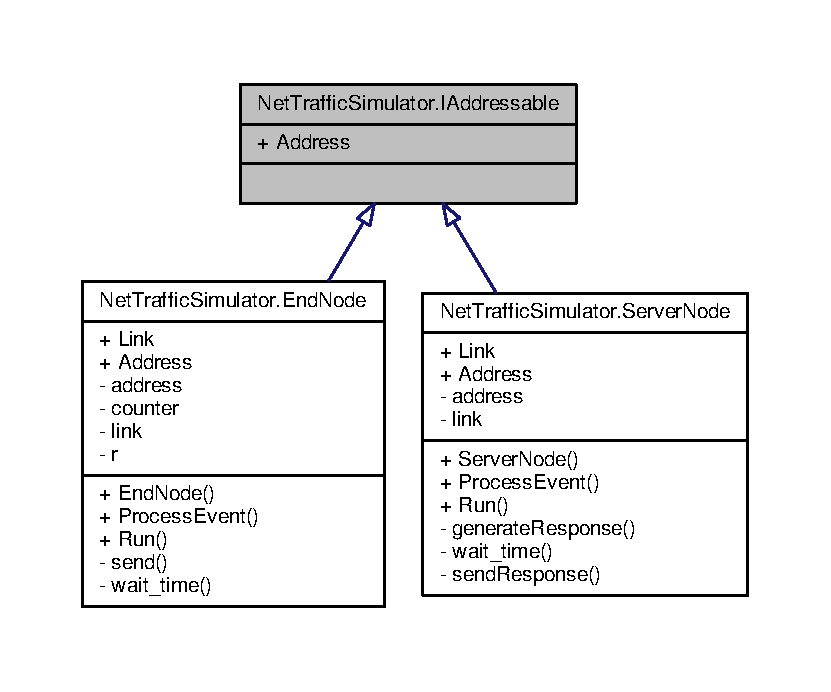
\includegraphics[width=350pt]{interfaceNetTrafficSimulator_1_1IAddressable__inherit__graph}
\end{center}
\end{figure}


Collaboration diagram for Net\-Traffic\-Simulator.\-I\-Addressable\-:\nopagebreak
\begin{figure}[H]
\begin{center}
\leavevmode
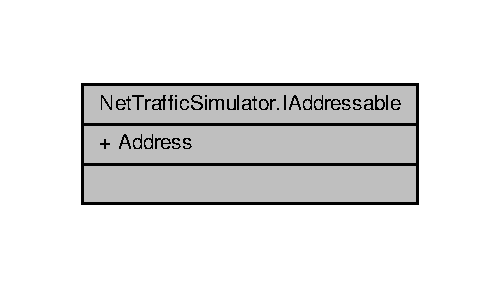
\includegraphics[width=240pt]{interfaceNetTrafficSimulator_1_1IAddressable__coll__graph}
\end{center}
\end{figure}
\subsection*{Properties}
\begin{DoxyCompactItemize}
\item 
int \hyperlink{interfaceNetTrafficSimulator_1_1IAddressable_a2d51a1c5896f8830489ea144070472fa}{Address}\hspace{0.3cm}{\ttfamily  \mbox{[}get\mbox{]}}
\end{DoxyCompactItemize}


\subsection{Property Documentation}
\hypertarget{interfaceNetTrafficSimulator_1_1IAddressable_a2d51a1c5896f8830489ea144070472fa}{\index{Net\-Traffic\-Simulator\-::\-I\-Addressable@{Net\-Traffic\-Simulator\-::\-I\-Addressable}!Address@{Address}}
\index{Address@{Address}!NetTrafficSimulator::IAddressable@{Net\-Traffic\-Simulator\-::\-I\-Addressable}}
\subsubsection[{Address}]{\setlength{\rightskip}{0pt plus 5cm}int Net\-Traffic\-Simulator.\-I\-Addressable.\-Address\hspace{0.3cm}{\ttfamily [get]}}}\label{interfaceNetTrafficSimulator_1_1IAddressable_a2d51a1c5896f8830489ea144070472fa}
The address of the addressable 

The documentation for this interface was generated from the following file\-:\begin{DoxyCompactItemize}
\item 
Net\-Traffic\-Simulator/\-Net\-Traffic\-Simulator/misc/\hyperlink{IAddressable_8cs}{I\-Addressable.\-cs}\end{DoxyCompactItemize}

\hypertarget{interfaceNetTrafficSimulator_1_1INamable}{\section{Net\-Traffic\-Simulator.\-I\-Namable Interface Reference}
\label{interfaceNetTrafficSimulator_1_1INamable}\index{Net\-Traffic\-Simulator.\-I\-Namable@{Net\-Traffic\-Simulator.\-I\-Namable}}
}


Inheritance diagram for Net\-Traffic\-Simulator.\-I\-Namable\-:
\nopagebreak
\begin{figure}[H]
\begin{center}
\leavevmode
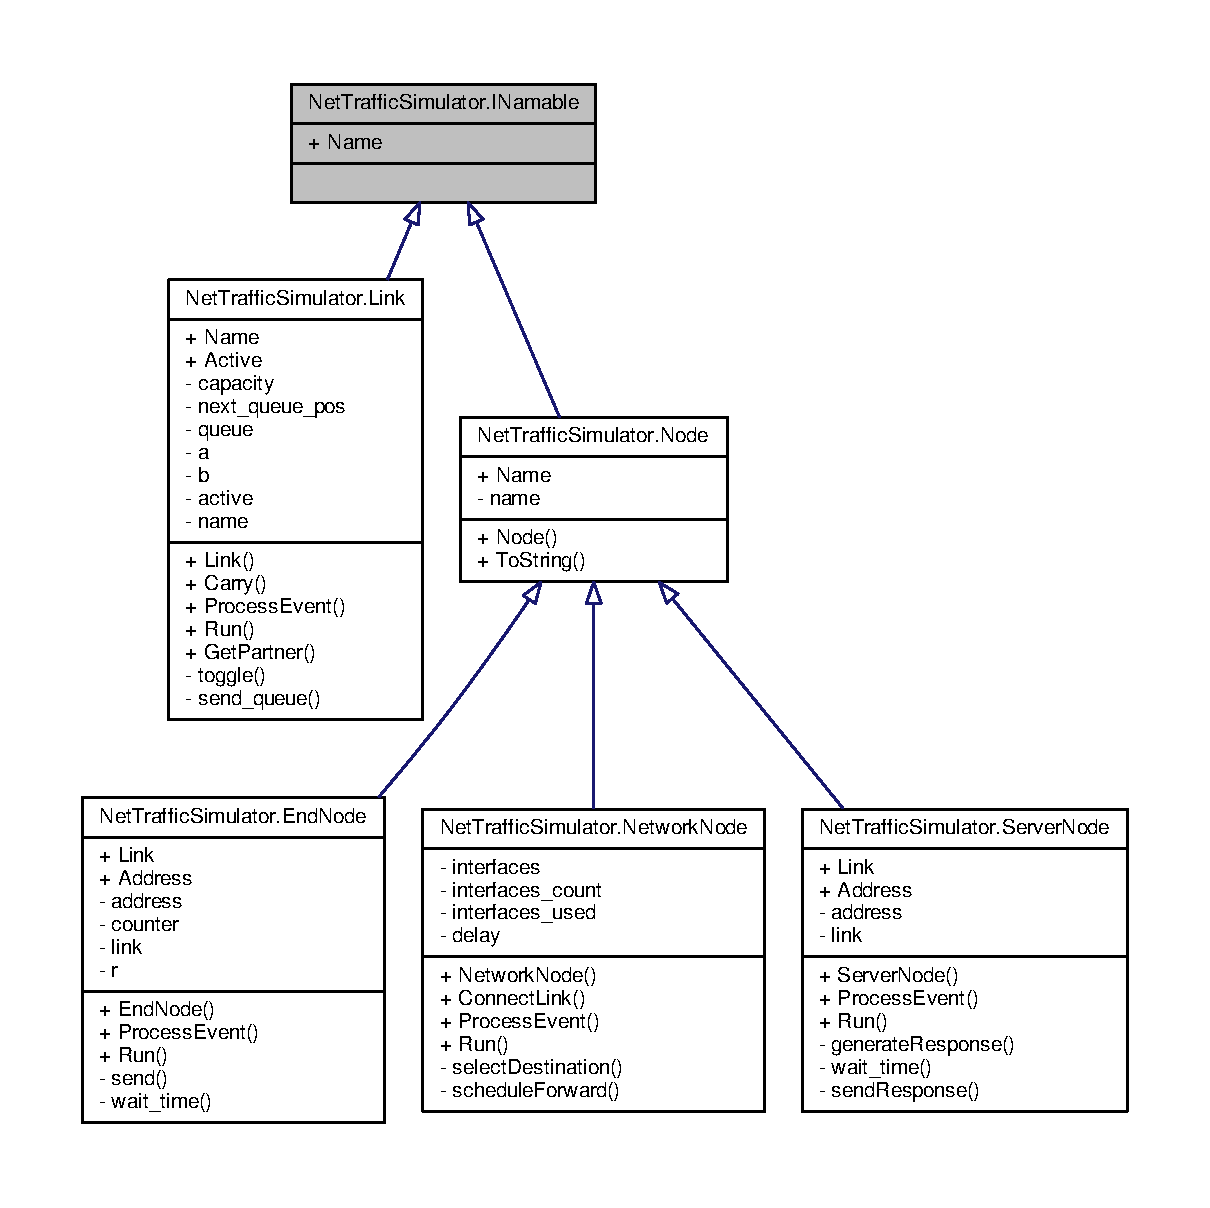
\includegraphics[width=350pt]{interfaceNetTrafficSimulator_1_1INamable__inherit__graph}
\end{center}
\end{figure}


Collaboration diagram for Net\-Traffic\-Simulator.\-I\-Namable\-:\nopagebreak
\begin{figure}[H]
\begin{center}
\leavevmode
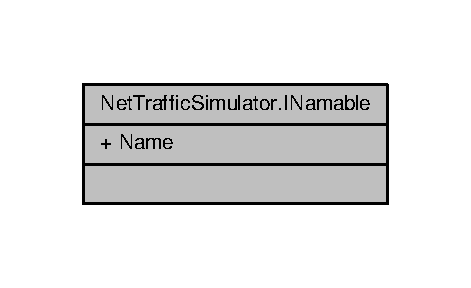
\includegraphics[width=226pt]{interfaceNetTrafficSimulator_1_1INamable__coll__graph}
\end{center}
\end{figure}
\subsection*{Properties}
\begin{DoxyCompactItemize}
\item 
string \hyperlink{interfaceNetTrafficSimulator_1_1INamable_a533eb537abe688050cc25a28fbcb9d3f}{Name}\hspace{0.3cm}{\ttfamily  \mbox{[}get\mbox{]}}
\end{DoxyCompactItemize}


\subsection{Property Documentation}
\hypertarget{interfaceNetTrafficSimulator_1_1INamable_a533eb537abe688050cc25a28fbcb9d3f}{\index{Net\-Traffic\-Simulator\-::\-I\-Namable@{Net\-Traffic\-Simulator\-::\-I\-Namable}!Name@{Name}}
\index{Name@{Name}!NetTrafficSimulator::INamable@{Net\-Traffic\-Simulator\-::\-I\-Namable}}
\subsubsection[{Name}]{\setlength{\rightskip}{0pt plus 5cm}string Net\-Traffic\-Simulator.\-I\-Namable.\-Name\hspace{0.3cm}{\ttfamily [get]}}}\label{interfaceNetTrafficSimulator_1_1INamable_a533eb537abe688050cc25a28fbcb9d3f}
Name of the Namable object instance 

The documentation for this interface was generated from the following file\-:\begin{DoxyCompactItemize}
\item 
Net\-Traffic\-Simulator/\-Net\-Traffic\-Simulator/misc/\hyperlink{INamable_8cs}{I\-Namable.\-cs}\end{DoxyCompactItemize}

\hypertarget{classNetTrafficSimulator_1_1Link}{\section{Net\-Traffic\-Simulator.\-Link Class Reference}
\label{classNetTrafficSimulator_1_1Link}\index{Net\-Traffic\-Simulator.\-Link@{Net\-Traffic\-Simulator.\-Link}}
}


Inheritance diagram for Net\-Traffic\-Simulator.\-Link\-:
\nopagebreak
\begin{figure}[H]
\begin{center}
\leavevmode
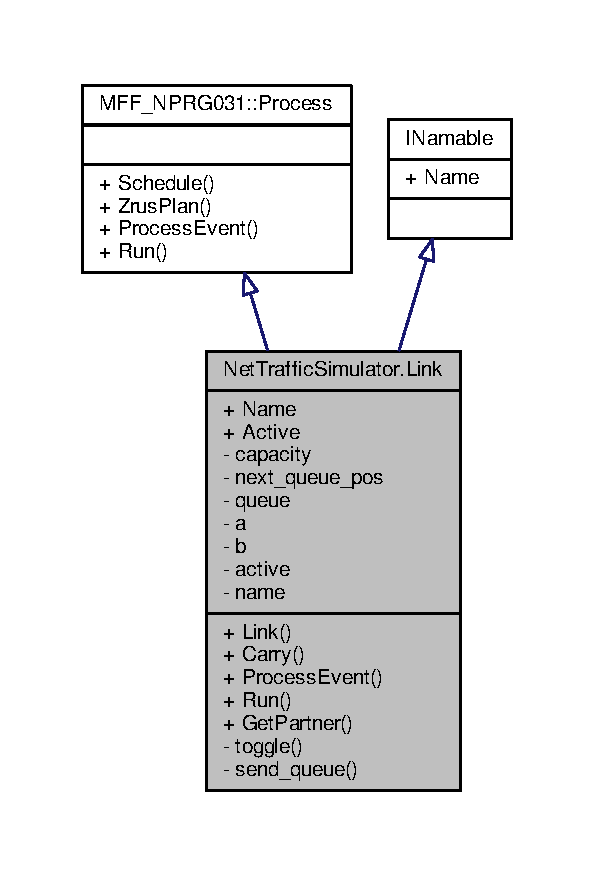
\includegraphics[width=350pt]{classNetTrafficSimulator_1_1Link__inherit__graph}
\end{center}
\end{figure}


Collaboration diagram for Net\-Traffic\-Simulator.\-Link\-:
\nopagebreak
\begin{figure}[H]
\begin{center}
\leavevmode
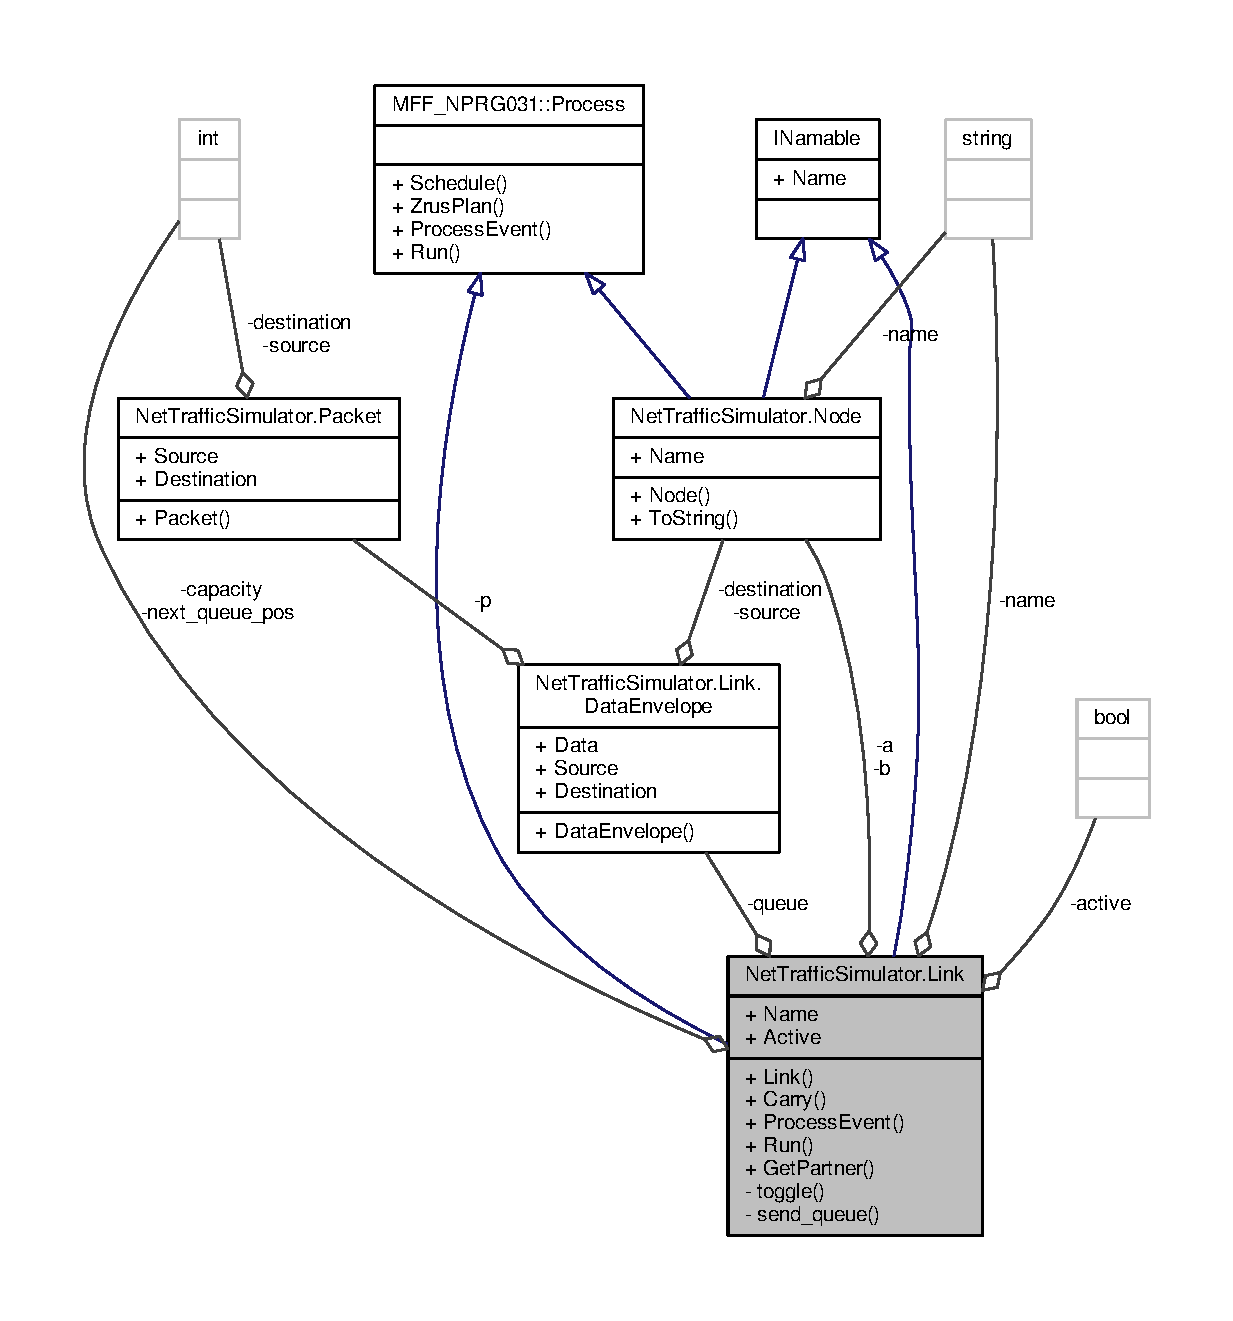
\includegraphics[width=350pt]{classNetTrafficSimulator_1_1Link__coll__graph}
\end{center}
\end{figure}
\subsection*{Classes}
\begin{DoxyCompactItemize}
\item 
class \hyperlink{classNetTrafficSimulator_1_1Link_1_1DataEnvelope}{Data\-Envelope}
\end{DoxyCompactItemize}
\subsection*{Public Member Functions}
\begin{DoxyCompactItemize}
\item 
\hyperlink{classNetTrafficSimulator_1_1Link_a83847c253f988b59e7224d665901449b}{Link} (String \hyperlink{classNetTrafficSimulator_1_1Link_af5a2835b585c255fbc6584f2f5388be8}{name}, int \hyperlink{classNetTrafficSimulator_1_1Link_a24a004105c985c4e5ee64e4c839b1915}{capacity}, \hyperlink{classNetTrafficSimulator_1_1Node}{Node} \hyperlink{classNetTrafficSimulator_1_1Link_a4b7875d945423d1f64c31d8156a3308d}{a}, \hyperlink{classNetTrafficSimulator_1_1Node}{Node} \hyperlink{classNetTrafficSimulator_1_1Link_af85461b8b8d35adb1d8fc80849c0717d}{b})
\item 
void \hyperlink{classNetTrafficSimulator_1_1Link_a51bfc5e94e05941d8302c5552e36f1a3}{Carry} (\hyperlink{classNetTrafficSimulator_1_1Packet}{Packet} p, \hyperlink{classNetTrafficSimulator_1_1Node}{Node} origin, \hyperlink{classNetTrafficSimulator_1_1Node}{Node} destination)
\item 
override void \hyperlink{classNetTrafficSimulator_1_1Link_a953900c6d1064af45c99b9533eadeafe}{Process\-Event} (\hyperlink{classMFF__NPRG031_1_1State}{M\-F\-F\-\_\-\-N\-P\-R\-G031.\-State} state, \hyperlink{classMFF__NPRG031_1_1Model}{M\-F\-F\-\_\-\-N\-P\-R\-G031.\-Model} model)
\item 
override void \hyperlink{classNetTrafficSimulator_1_1Link_a654d0221ce7490d08ad40a70887b80c8}{Run} (\hyperlink{classMFF__NPRG031_1_1Model}{M\-F\-F\-\_\-\-N\-P\-R\-G031.\-Model} m)
\item 
\hyperlink{classNetTrafficSimulator_1_1Node}{Node} \hyperlink{classNetTrafficSimulator_1_1Link_a45cd71692f0fc8b76d4ae5f53d14580a}{Get\-Partner} (\hyperlink{classNetTrafficSimulator_1_1Node}{Node} x)
\item 
Dictionary$<$ string, object $>$ \hyperlink{classNetTrafficSimulator_1_1Link_aa0d6e4b0e7f61acda461b4d1eab0f1fd}{Get\-Results} (\hyperlink{classMFF__NPRG031_1_1Model}{M\-F\-F\-\_\-\-N\-P\-R\-G031.\-Model} model)
\end{DoxyCompactItemize}
\subsection*{Properties}
\begin{DoxyCompactItemize}
\item 
string \hyperlink{classNetTrafficSimulator_1_1Link_ac6510bbaac975c237d4dab9b492b5cfe}{Name}\hspace{0.3cm}{\ttfamily  \mbox{[}get\mbox{]}}
\item 
bool \hyperlink{classNetTrafficSimulator_1_1Link_af5dbc33cd8e78697ce401ad2520877e8}{Active}\hspace{0.3cm}{\ttfamily  \mbox{[}get\mbox{]}}
\end{DoxyCompactItemize}
\subsection*{Private Member Functions}
\begin{DoxyCompactItemize}
\item 
bool \hyperlink{classNetTrafficSimulator_1_1Link_a06d3c8e29b67ae95c9d854c97cf48d1e}{toggle} ()
\item 
void \hyperlink{classNetTrafficSimulator_1_1Link_a4ca4f2df795e1a3e814af806a176789d}{send\-\_\-queue} (\hyperlink{classMFF__NPRG031_1_1Model}{M\-F\-F\-\_\-\-N\-P\-R\-G031.\-Model} model)
\end{DoxyCompactItemize}
\subsection*{Private Attributes}
\begin{DoxyCompactItemize}
\item 
int \hyperlink{classNetTrafficSimulator_1_1Link_a0374f1c17ad827ae00d53d41b1893a9e}{dropped}
\item 
int \hyperlink{classNetTrafficSimulator_1_1Link_a9c09033d252b42f62a3857397c06e320}{active\-\_\-time}
\item 
int \hyperlink{classNetTrafficSimulator_1_1Link_a2359ef316a04da7a0170827792a8b703}{inactive\-\_\-time}
\item 
int \hyperlink{classNetTrafficSimulator_1_1Link_ada7cc15d14a2c0d9111e91a96656e973}{carried}
\item 
int \hyperlink{classNetTrafficSimulator_1_1Link_a1b4280184e08f88565060c4786d5033b}{last\-\_\-process}
\item 
int \hyperlink{classNetTrafficSimulator_1_1Link_a24a004105c985c4e5ee64e4c839b1915}{capacity}
\item 
int \hyperlink{classNetTrafficSimulator_1_1Link_ae9f28a316a491bf4823314f5f794484a}{next\-\_\-queue\-\_\-pos}
\item 
\hyperlink{classNetTrafficSimulator_1_1Link_1_1DataEnvelope}{Data\-Envelope}\mbox{[}$\,$\mbox{]} \hyperlink{classNetTrafficSimulator_1_1Link_a0a9c8700a5fe5e22d7091587319886aa}{queue}
\item 
\hyperlink{classNetTrafficSimulator_1_1Node}{Node} \hyperlink{classNetTrafficSimulator_1_1Link_a4b7875d945423d1f64c31d8156a3308d}{a}
\item 
\hyperlink{classNetTrafficSimulator_1_1Node}{Node} \hyperlink{classNetTrafficSimulator_1_1Link_af85461b8b8d35adb1d8fc80849c0717d}{b}
\item 
bool \hyperlink{classNetTrafficSimulator_1_1Link_a1026cabe177ffe17054699706dea1452}{active}
\item 
string \hyperlink{classNetTrafficSimulator_1_1Link_af5a2835b585c255fbc6584f2f5388be8}{name}
\end{DoxyCompactItemize}


\subsection{Constructor \& Destructor Documentation}
\hypertarget{classNetTrafficSimulator_1_1Link_a83847c253f988b59e7224d665901449b}{\index{Net\-Traffic\-Simulator\-::\-Link@{Net\-Traffic\-Simulator\-::\-Link}!Link@{Link}}
\index{Link@{Link}!NetTrafficSimulator::Link@{Net\-Traffic\-Simulator\-::\-Link}}
\subsubsection[{Link}]{\setlength{\rightskip}{0pt plus 5cm}Net\-Traffic\-Simulator.\-Link.\-Link (
\begin{DoxyParamCaption}
\item[{String}]{name, }
\item[{int}]{capacity, }
\item[{{\bf Node}}]{a, }
\item[{{\bf Node}}]{b}
\end{DoxyParamCaption}
)\hspace{0.3cm}{\ttfamily [inline]}}}\label{classNetTrafficSimulator_1_1Link_a83847c253f988b59e7224d665901449b}
Creates a new link between two nodes with given capacity which specifies how many data the link will be able to deliver per time unit 
\begin{DoxyParams}{Parameters}
{\em capacity} & how many data a link can deliver per time unit \\
\hline
{\em a} & node at one end \\
\hline
{\em b} & node at other end \\
\hline
\end{DoxyParams}


\subsection{Member Function Documentation}
\hypertarget{classNetTrafficSimulator_1_1Link_a51bfc5e94e05941d8302c5552e36f1a3}{\index{Net\-Traffic\-Simulator\-::\-Link@{Net\-Traffic\-Simulator\-::\-Link}!Carry@{Carry}}
\index{Carry@{Carry}!NetTrafficSimulator::Link@{Net\-Traffic\-Simulator\-::\-Link}}
\subsubsection[{Carry}]{\setlength{\rightskip}{0pt plus 5cm}void Net\-Traffic\-Simulator.\-Link.\-Carry (
\begin{DoxyParamCaption}
\item[{{\bf Packet}}]{p, }
\item[{{\bf Node}}]{origin, }
\item[{{\bf Node}}]{destination}
\end{DoxyParamCaption}
)\hspace{0.3cm}{\ttfamily [inline]}}}\label{classNetTrafficSimulator_1_1Link_a51bfc5e94e05941d8302c5552e36f1a3}
\hyperlink{classNetTrafficSimulator_1_1Link}{Link} is capable of carrying specified amount of packets each step of simulation This method verifies origin and destination match link definition and then, if there is availability to send the particular packet in the next step, will create a data envelope object and store it in a queue If the link is unable to sent the packet in the next step of simulation, the packet will be lost 
\begin{DoxyParams}{Parameters}
{\em p} & \hyperlink{classNetTrafficSimulator_1_1Packet}{Packet} to transfer \\
\hline
{\em origin} & \hyperlink{classNetTrafficSimulator_1_1Node}{Node} sending the packet \\
\hline
{\em destination} & \hyperlink{classNetTrafficSimulator_1_1Node}{Node} receiving the packet on the other end \\
\hline
\end{DoxyParams}

\begin{DoxyExceptions}{Exceptions}
{\em Argument\-Exception} & if origin and destination are not nodes specified in the consructor regardless of order \\
\hline
\end{DoxyExceptions}
\hypertarget{classNetTrafficSimulator_1_1Link_a45cd71692f0fc8b76d4ae5f53d14580a}{\index{Net\-Traffic\-Simulator\-::\-Link@{Net\-Traffic\-Simulator\-::\-Link}!Get\-Partner@{Get\-Partner}}
\index{Get\-Partner@{Get\-Partner}!NetTrafficSimulator::Link@{Net\-Traffic\-Simulator\-::\-Link}}
\subsubsection[{Get\-Partner}]{\setlength{\rightskip}{0pt plus 5cm}{\bf Node} Net\-Traffic\-Simulator.\-Link.\-Get\-Partner (
\begin{DoxyParamCaption}
\item[{{\bf Node}}]{x}
\end{DoxyParamCaption}
)\hspace{0.3cm}{\ttfamily [inline]}}}\label{classNetTrafficSimulator_1_1Link_a45cd71692f0fc8b76d4ae5f53d14580a}
For given node return the second one of the pair 
\begin{DoxyParams}{Parameters}
{\em x} & a node of the pair specified in the constructor \\
\hline
\end{DoxyParams}
\begin{DoxyReturn}{Returns}
the second node of the pair specified in the constructor 
\end{DoxyReturn}

\begin{DoxyExceptions}{Exceptions}
{\em Argument\-Exception} & if x is not a node specified in the constructor \\
\hline
\end{DoxyExceptions}


Here is the caller graph for this function\-:\nopagebreak
\begin{figure}[H]
\begin{center}
\leavevmode
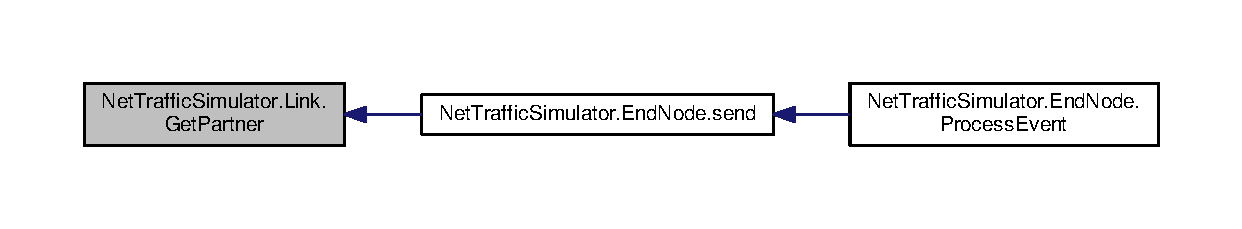
\includegraphics[width=350pt]{classNetTrafficSimulator_1_1Link_a45cd71692f0fc8b76d4ae5f53d14580a_icgraph}
\end{center}
\end{figure}


\hypertarget{classNetTrafficSimulator_1_1Link_aa0d6e4b0e7f61acda461b4d1eab0f1fd}{\index{Net\-Traffic\-Simulator\-::\-Link@{Net\-Traffic\-Simulator\-::\-Link}!Get\-Results@{Get\-Results}}
\index{Get\-Results@{Get\-Results}!NetTrafficSimulator::Link@{Net\-Traffic\-Simulator\-::\-Link}}
\subsubsection[{Get\-Results}]{\setlength{\rightskip}{0pt plus 5cm}Dictionary$<$string,object$>$ Net\-Traffic\-Simulator.\-Link.\-Get\-Results (
\begin{DoxyParamCaption}
\item[{{\bf M\-F\-F\-\_\-\-N\-P\-R\-G031.\-Model}}]{model}
\end{DoxyParamCaption}
)\hspace{0.3cm}{\ttfamily [inline]}}}\label{classNetTrafficSimulator_1_1Link_aa0d6e4b0e7f61acda461b4d1eab0f1fd}
Provide results measured during simulation for populating a result model \begin{DoxyReturn}{Returns}
Dictionary, where string is a key representing a human-\/readable description of measured data and object is value measured 
\end{DoxyReturn}


Implements \hyperlink{interfaceNetTrafficSimulator_1_1IResultProvider_ac7053c11f509ba1c2f653cd952b05323}{Net\-Traffic\-Simulator.\-I\-Result\-Provider}.

\hypertarget{classNetTrafficSimulator_1_1Link_a953900c6d1064af45c99b9533eadeafe}{\index{Net\-Traffic\-Simulator\-::\-Link@{Net\-Traffic\-Simulator\-::\-Link}!Process\-Event@{Process\-Event}}
\index{Process\-Event@{Process\-Event}!NetTrafficSimulator::Link@{Net\-Traffic\-Simulator\-::\-Link}}
\subsubsection[{Process\-Event}]{\setlength{\rightskip}{0pt plus 5cm}override void Net\-Traffic\-Simulator.\-Link.\-Process\-Event (
\begin{DoxyParamCaption}
\item[{{\bf M\-F\-F\-\_\-\-N\-P\-R\-G031.\-State}}]{state, }
\item[{{\bf M\-F\-F\-\_\-\-N\-P\-R\-G031.\-Model}}]{model}
\end{DoxyParamCaption}
)\hspace{0.3cm}{\ttfamily [inline]}, {\ttfamily [virtual]}}}\label{classNetTrafficSimulator_1_1Link_a953900c6d1064af45c99b9533eadeafe}
Abstract method Process\-Event for process to react on event hapened 
\begin{DoxyParams}{Parameters}
{\em state} & In what state the process is now \\
\hline
{\em model} & Our simulation model \\
\hline
\end{DoxyParams}


Implements \hyperlink{classMFF__NPRG031_1_1Process_acb58d206e76c177264614d88f1818fdc}{M\-F\-F\-\_\-\-N\-P\-R\-G031.\-Process}.



Here is the call graph for this function\-:\nopagebreak
\begin{figure}[H]
\begin{center}
\leavevmode
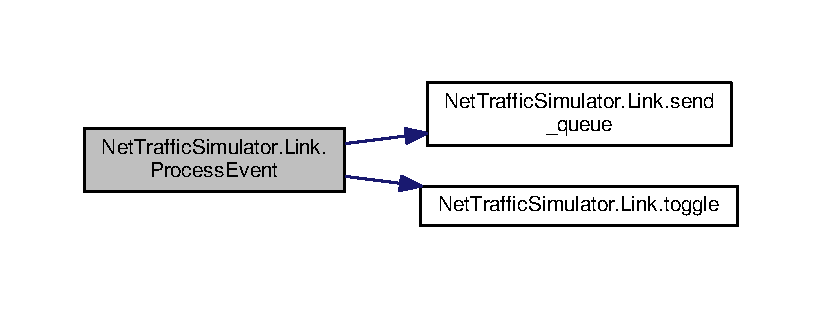
\includegraphics[width=350pt]{classNetTrafficSimulator_1_1Link_a953900c6d1064af45c99b9533eadeafe_cgraph}
\end{center}
\end{figure}


\hypertarget{classNetTrafficSimulator_1_1Link_a654d0221ce7490d08ad40a70887b80c8}{\index{Net\-Traffic\-Simulator\-::\-Link@{Net\-Traffic\-Simulator\-::\-Link}!Run@{Run}}
\index{Run@{Run}!NetTrafficSimulator::Link@{Net\-Traffic\-Simulator\-::\-Link}}
\subsubsection[{Run}]{\setlength{\rightskip}{0pt plus 5cm}override void Net\-Traffic\-Simulator.\-Link.\-Run (
\begin{DoxyParamCaption}
\item[{{\bf M\-F\-F\-\_\-\-N\-P\-R\-G031.\-Model}}]{m}
\end{DoxyParamCaption}
)\hspace{0.3cm}{\ttfamily [inline]}, {\ttfamily [virtual]}}}\label{classNetTrafficSimulator_1_1Link_a654d0221ce7490d08ad40a70887b80c8}
Initial set up 
\begin{DoxyParams}{Parameters}
{\em m} & Model given \\
\hline
\end{DoxyParams}


Implements \hyperlink{classMFF__NPRG031_1_1Process_ad0e440dee98ba26c59ab22a60ebcafdd}{M\-F\-F\-\_\-\-N\-P\-R\-G031.\-Process}.

\hypertarget{classNetTrafficSimulator_1_1Link_a4ca4f2df795e1a3e814af806a176789d}{\index{Net\-Traffic\-Simulator\-::\-Link@{Net\-Traffic\-Simulator\-::\-Link}!send\-\_\-queue@{send\-\_\-queue}}
\index{send\-\_\-queue@{send\-\_\-queue}!NetTrafficSimulator::Link@{Net\-Traffic\-Simulator\-::\-Link}}
\subsubsection[{send\-\_\-queue}]{\setlength{\rightskip}{0pt plus 5cm}void Net\-Traffic\-Simulator.\-Link.\-send\-\_\-queue (
\begin{DoxyParamCaption}
\item[{{\bf M\-F\-F\-\_\-\-N\-P\-R\-G031.\-Model}}]{model}
\end{DoxyParamCaption}
)\hspace{0.3cm}{\ttfamily [inline]}, {\ttfamily [private]}}}\label{classNetTrafficSimulator_1_1Link_a4ca4f2df795e1a3e814af806a176789d}
For each \hyperlink{classNetTrafficSimulator_1_1Link_1_1DataEnvelope}{Data\-Envelope} enqueued will schedule destination to R\-E\-C\-E\-I\-V\-E the data given at time T+1 and reset the queue for next step 
\begin{DoxyParams}{Parameters}
{\em model} & the Model \\
\hline
\end{DoxyParams}


Here is the caller graph for this function\-:\nopagebreak
\begin{figure}[H]
\begin{center}
\leavevmode
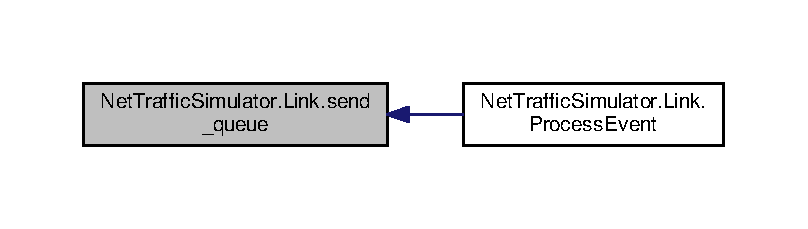
\includegraphics[width=350pt]{classNetTrafficSimulator_1_1Link_a4ca4f2df795e1a3e814af806a176789d_icgraph}
\end{center}
\end{figure}


\hypertarget{classNetTrafficSimulator_1_1Link_a06d3c8e29b67ae95c9d854c97cf48d1e}{\index{Net\-Traffic\-Simulator\-::\-Link@{Net\-Traffic\-Simulator\-::\-Link}!toggle@{toggle}}
\index{toggle@{toggle}!NetTrafficSimulator::Link@{Net\-Traffic\-Simulator\-::\-Link}}
\subsubsection[{toggle}]{\setlength{\rightskip}{0pt plus 5cm}bool Net\-Traffic\-Simulator.\-Link.\-toggle (
\begin{DoxyParamCaption}
{}
\end{DoxyParamCaption}
)\hspace{0.3cm}{\ttfamily [inline]}, {\ttfamily [private]}}}\label{classNetTrafficSimulator_1_1Link_a06d3c8e29b67ae95c9d854c97cf48d1e}


Here is the caller graph for this function\-:\nopagebreak
\begin{figure}[H]
\begin{center}
\leavevmode
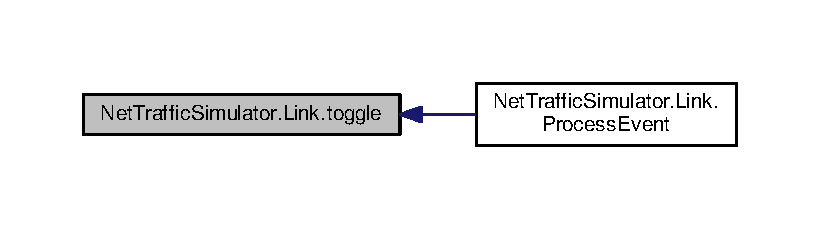
\includegraphics[width=350pt]{classNetTrafficSimulator_1_1Link_a06d3c8e29b67ae95c9d854c97cf48d1e_icgraph}
\end{center}
\end{figure}




\subsection{Member Data Documentation}
\hypertarget{classNetTrafficSimulator_1_1Link_a4b7875d945423d1f64c31d8156a3308d}{\index{Net\-Traffic\-Simulator\-::\-Link@{Net\-Traffic\-Simulator\-::\-Link}!a@{a}}
\index{a@{a}!NetTrafficSimulator::Link@{Net\-Traffic\-Simulator\-::\-Link}}
\subsubsection[{a}]{\setlength{\rightskip}{0pt plus 5cm}{\bf Node} Net\-Traffic\-Simulator.\-Link.\-a\hspace{0.3cm}{\ttfamily [private]}}}\label{classNetTrafficSimulator_1_1Link_a4b7875d945423d1f64c31d8156a3308d}
\hypertarget{classNetTrafficSimulator_1_1Link_a1026cabe177ffe17054699706dea1452}{\index{Net\-Traffic\-Simulator\-::\-Link@{Net\-Traffic\-Simulator\-::\-Link}!active@{active}}
\index{active@{active}!NetTrafficSimulator::Link@{Net\-Traffic\-Simulator\-::\-Link}}
\subsubsection[{active}]{\setlength{\rightskip}{0pt plus 5cm}bool Net\-Traffic\-Simulator.\-Link.\-active\hspace{0.3cm}{\ttfamily [private]}}}\label{classNetTrafficSimulator_1_1Link_a1026cabe177ffe17054699706dea1452}
\hypertarget{classNetTrafficSimulator_1_1Link_a9c09033d252b42f62a3857397c06e320}{\index{Net\-Traffic\-Simulator\-::\-Link@{Net\-Traffic\-Simulator\-::\-Link}!active\-\_\-time@{active\-\_\-time}}
\index{active\-\_\-time@{active\-\_\-time}!NetTrafficSimulator::Link@{Net\-Traffic\-Simulator\-::\-Link}}
\subsubsection[{active\-\_\-time}]{\setlength{\rightskip}{0pt plus 5cm}int Net\-Traffic\-Simulator.\-Link.\-active\-\_\-time\hspace{0.3cm}{\ttfamily [private]}}}\label{classNetTrafficSimulator_1_1Link_a9c09033d252b42f62a3857397c06e320}
\hypertarget{classNetTrafficSimulator_1_1Link_af85461b8b8d35adb1d8fc80849c0717d}{\index{Net\-Traffic\-Simulator\-::\-Link@{Net\-Traffic\-Simulator\-::\-Link}!b@{b}}
\index{b@{b}!NetTrafficSimulator::Link@{Net\-Traffic\-Simulator\-::\-Link}}
\subsubsection[{b}]{\setlength{\rightskip}{0pt plus 5cm}{\bf Node} Net\-Traffic\-Simulator.\-Link.\-b\hspace{0.3cm}{\ttfamily [private]}}}\label{classNetTrafficSimulator_1_1Link_af85461b8b8d35adb1d8fc80849c0717d}
\hypertarget{classNetTrafficSimulator_1_1Link_a24a004105c985c4e5ee64e4c839b1915}{\index{Net\-Traffic\-Simulator\-::\-Link@{Net\-Traffic\-Simulator\-::\-Link}!capacity@{capacity}}
\index{capacity@{capacity}!NetTrafficSimulator::Link@{Net\-Traffic\-Simulator\-::\-Link}}
\subsubsection[{capacity}]{\setlength{\rightskip}{0pt plus 5cm}int Net\-Traffic\-Simulator.\-Link.\-capacity\hspace{0.3cm}{\ttfamily [private]}}}\label{classNetTrafficSimulator_1_1Link_a24a004105c985c4e5ee64e4c839b1915}
\hypertarget{classNetTrafficSimulator_1_1Link_ada7cc15d14a2c0d9111e91a96656e973}{\index{Net\-Traffic\-Simulator\-::\-Link@{Net\-Traffic\-Simulator\-::\-Link}!carried@{carried}}
\index{carried@{carried}!NetTrafficSimulator::Link@{Net\-Traffic\-Simulator\-::\-Link}}
\subsubsection[{carried}]{\setlength{\rightskip}{0pt plus 5cm}int Net\-Traffic\-Simulator.\-Link.\-carried\hspace{0.3cm}{\ttfamily [private]}}}\label{classNetTrafficSimulator_1_1Link_ada7cc15d14a2c0d9111e91a96656e973}
\hypertarget{classNetTrafficSimulator_1_1Link_a0374f1c17ad827ae00d53d41b1893a9e}{\index{Net\-Traffic\-Simulator\-::\-Link@{Net\-Traffic\-Simulator\-::\-Link}!dropped@{dropped}}
\index{dropped@{dropped}!NetTrafficSimulator::Link@{Net\-Traffic\-Simulator\-::\-Link}}
\subsubsection[{dropped}]{\setlength{\rightskip}{0pt plus 5cm}int Net\-Traffic\-Simulator.\-Link.\-dropped\hspace{0.3cm}{\ttfamily [private]}}}\label{classNetTrafficSimulator_1_1Link_a0374f1c17ad827ae00d53d41b1893a9e}
\hypertarget{classNetTrafficSimulator_1_1Link_a2359ef316a04da7a0170827792a8b703}{\index{Net\-Traffic\-Simulator\-::\-Link@{Net\-Traffic\-Simulator\-::\-Link}!inactive\-\_\-time@{inactive\-\_\-time}}
\index{inactive\-\_\-time@{inactive\-\_\-time}!NetTrafficSimulator::Link@{Net\-Traffic\-Simulator\-::\-Link}}
\subsubsection[{inactive\-\_\-time}]{\setlength{\rightskip}{0pt plus 5cm}int Net\-Traffic\-Simulator.\-Link.\-inactive\-\_\-time\hspace{0.3cm}{\ttfamily [private]}}}\label{classNetTrafficSimulator_1_1Link_a2359ef316a04da7a0170827792a8b703}
\hypertarget{classNetTrafficSimulator_1_1Link_a1b4280184e08f88565060c4786d5033b}{\index{Net\-Traffic\-Simulator\-::\-Link@{Net\-Traffic\-Simulator\-::\-Link}!last\-\_\-process@{last\-\_\-process}}
\index{last\-\_\-process@{last\-\_\-process}!NetTrafficSimulator::Link@{Net\-Traffic\-Simulator\-::\-Link}}
\subsubsection[{last\-\_\-process}]{\setlength{\rightskip}{0pt plus 5cm}int Net\-Traffic\-Simulator.\-Link.\-last\-\_\-process\hspace{0.3cm}{\ttfamily [private]}}}\label{classNetTrafficSimulator_1_1Link_a1b4280184e08f88565060c4786d5033b}
\hypertarget{classNetTrafficSimulator_1_1Link_af5a2835b585c255fbc6584f2f5388be8}{\index{Net\-Traffic\-Simulator\-::\-Link@{Net\-Traffic\-Simulator\-::\-Link}!name@{name}}
\index{name@{name}!NetTrafficSimulator::Link@{Net\-Traffic\-Simulator\-::\-Link}}
\subsubsection[{name}]{\setlength{\rightskip}{0pt plus 5cm}string Net\-Traffic\-Simulator.\-Link.\-name\hspace{0.3cm}{\ttfamily [private]}}}\label{classNetTrafficSimulator_1_1Link_af5a2835b585c255fbc6584f2f5388be8}
\hypertarget{classNetTrafficSimulator_1_1Link_ae9f28a316a491bf4823314f5f794484a}{\index{Net\-Traffic\-Simulator\-::\-Link@{Net\-Traffic\-Simulator\-::\-Link}!next\-\_\-queue\-\_\-pos@{next\-\_\-queue\-\_\-pos}}
\index{next\-\_\-queue\-\_\-pos@{next\-\_\-queue\-\_\-pos}!NetTrafficSimulator::Link@{Net\-Traffic\-Simulator\-::\-Link}}
\subsubsection[{next\-\_\-queue\-\_\-pos}]{\setlength{\rightskip}{0pt plus 5cm}int Net\-Traffic\-Simulator.\-Link.\-next\-\_\-queue\-\_\-pos\hspace{0.3cm}{\ttfamily [private]}}}\label{classNetTrafficSimulator_1_1Link_ae9f28a316a491bf4823314f5f794484a}
\hypertarget{classNetTrafficSimulator_1_1Link_a0a9c8700a5fe5e22d7091587319886aa}{\index{Net\-Traffic\-Simulator\-::\-Link@{Net\-Traffic\-Simulator\-::\-Link}!queue@{queue}}
\index{queue@{queue}!NetTrafficSimulator::Link@{Net\-Traffic\-Simulator\-::\-Link}}
\subsubsection[{queue}]{\setlength{\rightskip}{0pt plus 5cm}{\bf Data\-Envelope} \mbox{[}$\,$\mbox{]} Net\-Traffic\-Simulator.\-Link.\-queue\hspace{0.3cm}{\ttfamily [private]}}}\label{classNetTrafficSimulator_1_1Link_a0a9c8700a5fe5e22d7091587319886aa}


\subsection{Property Documentation}
\hypertarget{classNetTrafficSimulator_1_1Link_af5dbc33cd8e78697ce401ad2520877e8}{\index{Net\-Traffic\-Simulator\-::\-Link@{Net\-Traffic\-Simulator\-::\-Link}!Active@{Active}}
\index{Active@{Active}!NetTrafficSimulator::Link@{Net\-Traffic\-Simulator\-::\-Link}}
\subsubsection[{Active}]{\setlength{\rightskip}{0pt plus 5cm}bool Net\-Traffic\-Simulator.\-Link.\-Active\hspace{0.3cm}{\ttfamily [get]}}}\label{classNetTrafficSimulator_1_1Link_af5dbc33cd8e78697ce401ad2520877e8}
\hyperlink{classNetTrafficSimulator_1_1Link}{Link} is active if both nodes provided in constructor are not null and this state was not changed as result of toggle \hypertarget{classNetTrafficSimulator_1_1Link_ac6510bbaac975c237d4dab9b492b5cfe}{\index{Net\-Traffic\-Simulator\-::\-Link@{Net\-Traffic\-Simulator\-::\-Link}!Name@{Name}}
\index{Name@{Name}!NetTrafficSimulator::Link@{Net\-Traffic\-Simulator\-::\-Link}}
\subsubsection[{Name}]{\setlength{\rightskip}{0pt plus 5cm}string Net\-Traffic\-Simulator.\-Link.\-Name\hspace{0.3cm}{\ttfamily [get]}}}\label{classNetTrafficSimulator_1_1Link_ac6510bbaac975c237d4dab9b492b5cfe}
Human readable link name 

The documentation for this class was generated from the following file\-:\begin{DoxyCompactItemize}
\item 
Net\-Traffic\-Simulator/\-Net\-Traffic\-Simulator/framework/extension/\hyperlink{Link_8cs}{Link.\-cs}\end{DoxyCompactItemize}

\hypertarget{classNetTrafficSimulator_1_1MainClass}{\section{Net\-Traffic\-Simulator.\-Main\-Class Class Reference}
\label{classNetTrafficSimulator_1_1MainClass}\index{Net\-Traffic\-Simulator.\-Main\-Class@{Net\-Traffic\-Simulator.\-Main\-Class}}
}
\subsection*{Static Public Member Functions}
\begin{DoxyCompactItemize}
\item 
static void \hyperlink{classNetTrafficSimulator_1_1MainClass_a966b297e036542e72891d524accf8f3e}{Main} (string\mbox{[}$\,$\mbox{]} args)
\end{DoxyCompactItemize}


\subsection{Member Function Documentation}
\hypertarget{classNetTrafficSimulator_1_1MainClass_a966b297e036542e72891d524accf8f3e}{\index{Net\-Traffic\-Simulator\-::\-Main\-Class@{Net\-Traffic\-Simulator\-::\-Main\-Class}!Main@{Main}}
\index{Main@{Main}!NetTrafficSimulator::MainClass@{Net\-Traffic\-Simulator\-::\-Main\-Class}}
\subsubsection[{Main}]{\setlength{\rightskip}{0pt plus 5cm}static void Net\-Traffic\-Simulator.\-Main\-Class.\-Main (
\begin{DoxyParamCaption}
\item[{string\mbox{[}$\,$\mbox{]}}]{args}
\end{DoxyParamCaption}
)\hspace{0.3cm}{\ttfamily [inline]}, {\ttfamily [static]}}}\label{classNetTrafficSimulator_1_1MainClass_a966b297e036542e72891d524accf8f3e}


The documentation for this class was generated from the following file\-:\begin{DoxyCompactItemize}
\item 
Net\-Traffic\-Simulator/\-Net\-Traffic\-Simulator/\hyperlink{Program_8cs}{Program.\-cs}\end{DoxyCompactItemize}

\hypertarget{classMainWindow}{\section{Main\-Window Class Reference}
\label{classMainWindow}\index{Main\-Window@{Main\-Window}}
}


Inheritance diagram for Main\-Window\-:\nopagebreak
\begin{figure}[H]
\begin{center}
\leavevmode
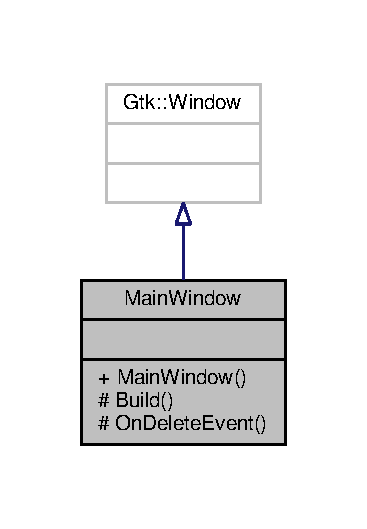
\includegraphics[width=176pt]{classMainWindow__inherit__graph}
\end{center}
\end{figure}


Collaboration diagram for Main\-Window\-:\nopagebreak
\begin{figure}[H]
\begin{center}
\leavevmode
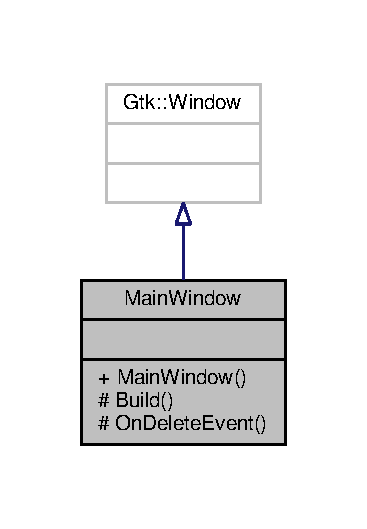
\includegraphics[width=176pt]{classMainWindow__coll__graph}
\end{center}
\end{figure}
\subsection*{Public Member Functions}
\begin{DoxyCompactItemize}
\item 
\hyperlink{classMainWindow_af607d50e4d1b04d3c494661489283f45}{Main\-Window} ()
\end{DoxyCompactItemize}
\subsection*{Protected Member Functions}
\begin{DoxyCompactItemize}
\item 
virtual void \hyperlink{classMainWindow_a952a77b964806830814cf4cdfbb2f0b9}{Build} ()
\item 
void \hyperlink{classMainWindow_a64bdcb29cebb58957790da1ee2733fe1}{On\-Delete\-Event} (object sender, Delete\-Event\-Args a)
\end{DoxyCompactItemize}


\subsection{Constructor \& Destructor Documentation}
\hypertarget{classMainWindow_af607d50e4d1b04d3c494661489283f45}{\index{Main\-Window@{Main\-Window}!Main\-Window@{Main\-Window}}
\index{Main\-Window@{Main\-Window}!MainWindow@{Main\-Window}}
\subsubsection[{Main\-Window}]{\setlength{\rightskip}{0pt plus 5cm}Main\-Window.\-Main\-Window (
\begin{DoxyParamCaption}
{}
\end{DoxyParamCaption}
)\hspace{0.3cm}{\ttfamily [inline]}}}\label{classMainWindow_af607d50e4d1b04d3c494661489283f45}


Here is the call graph for this function\-:\nopagebreak
\begin{figure}[H]
\begin{center}
\leavevmode
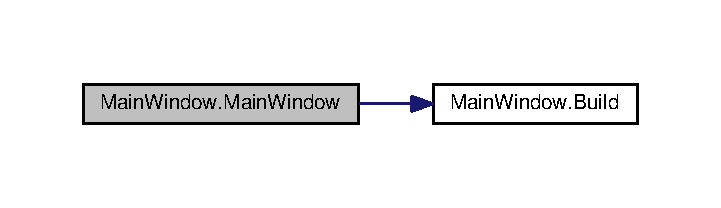
\includegraphics[width=346pt]{classMainWindow_af607d50e4d1b04d3c494661489283f45_cgraph}
\end{center}
\end{figure}




\subsection{Member Function Documentation}
\hypertarget{classMainWindow_a952a77b964806830814cf4cdfbb2f0b9}{\index{Main\-Window@{Main\-Window}!Build@{Build}}
\index{Build@{Build}!MainWindow@{Main\-Window}}
\subsubsection[{Build}]{\setlength{\rightskip}{0pt plus 5cm}virtual void Main\-Window.\-Build (
\begin{DoxyParamCaption}
{}
\end{DoxyParamCaption}
)\hspace{0.3cm}{\ttfamily [inline]}, {\ttfamily [protected]}, {\ttfamily [virtual]}}}\label{classMainWindow_a952a77b964806830814cf4cdfbb2f0b9}


Here is the caller graph for this function\-:\nopagebreak
\begin{figure}[H]
\begin{center}
\leavevmode
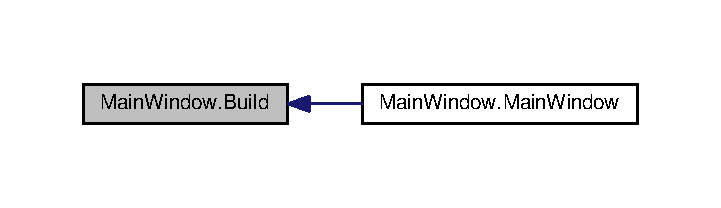
\includegraphics[width=346pt]{classMainWindow_a952a77b964806830814cf4cdfbb2f0b9_icgraph}
\end{center}
\end{figure}


\hypertarget{classMainWindow_a64bdcb29cebb58957790da1ee2733fe1}{\index{Main\-Window@{Main\-Window}!On\-Delete\-Event@{On\-Delete\-Event}}
\index{On\-Delete\-Event@{On\-Delete\-Event}!MainWindow@{Main\-Window}}
\subsubsection[{On\-Delete\-Event}]{\setlength{\rightskip}{0pt plus 5cm}void Main\-Window.\-On\-Delete\-Event (
\begin{DoxyParamCaption}
\item[{object}]{sender, }
\item[{Delete\-Event\-Args}]{a}
\end{DoxyParamCaption}
)\hspace{0.3cm}{\ttfamily [inline]}, {\ttfamily [protected]}}}\label{classMainWindow_a64bdcb29cebb58957790da1ee2733fe1}


The documentation for this class was generated from the following file\-:\begin{DoxyCompactItemize}
\item 
Net\-Traffic\-Simulator/\-Net\-Traffic\-Simulator/gtk-\/gui/\hyperlink{gtk-gui_2MainWindow_8cs}{Main\-Window.\-cs}\end{DoxyCompactItemize}

\hypertarget{classMFF__NPRG031_1_1Model}{\section{M\-F\-F\-\_\-\-N\-P\-R\-G031.\-Model Class Reference}
\label{classMFF__NPRG031_1_1Model}\index{M\-F\-F\-\_\-\-N\-P\-R\-G031.\-Model@{M\-F\-F\-\_\-\-N\-P\-R\-G031.\-Model}}
}


Collaboration diagram for M\-F\-F\-\_\-\-N\-P\-R\-G031.\-Model\-:\nopagebreak
\begin{figure}[H]
\begin{center}
\leavevmode
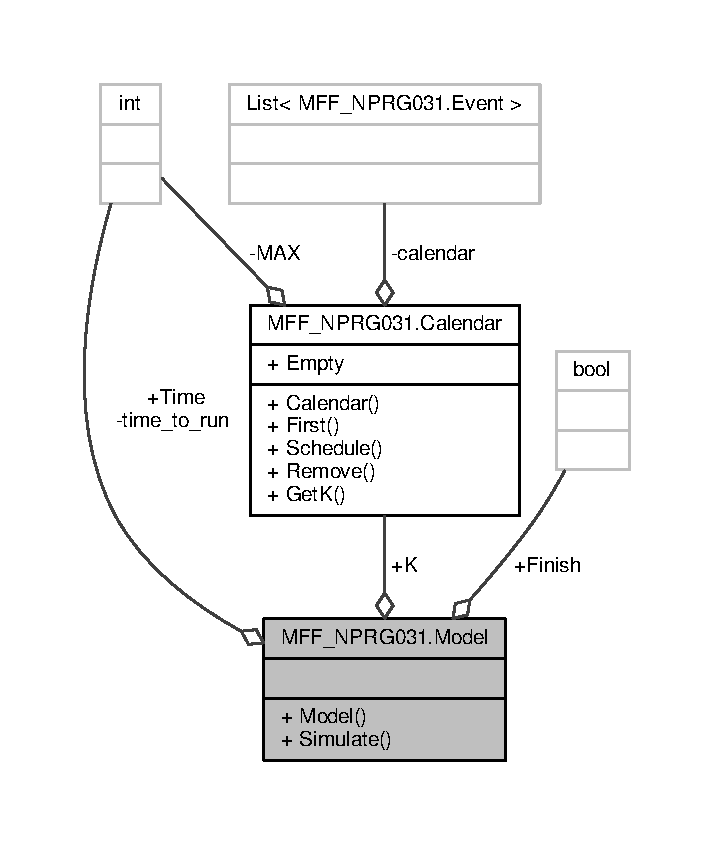
\includegraphics[width=342pt]{classMFF__NPRG031_1_1Model__coll__graph}
\end{center}
\end{figure}
\subsection*{Public Member Functions}
\begin{DoxyCompactItemize}
\item 
\hyperlink{classMFF__NPRG031_1_1Model_ada9504f66da371eebcf2c588b3da935f}{Model} (int \hyperlink{classMFF__NPRG031_1_1Model_a1e2a81337bc96f78f6336be46cdf0263}{time\-\_\-to\-\_\-run})
\item 
int \hyperlink{classMFF__NPRG031_1_1Model_a8ebc56d74c6e2c7e7481a9c413a27254}{Simulate} ()
\end{DoxyCompactItemize}
\subsection*{Public Attributes}
\begin{DoxyCompactItemize}
\item 
\hyperlink{classMFF__NPRG031_1_1Calendar}{Calendar} \hyperlink{classMFF__NPRG031_1_1Model_a233a1b86d155560a2c51526a5eac7222}{K}
\item 
bool \hyperlink{classMFF__NPRG031_1_1Model_ab1ba01c979484275f2e4707ea8cdbaa3}{Finish}
\item 
int \hyperlink{classMFF__NPRG031_1_1Model_a1e8fd74f1d69f6c7c71d5d1e08388e8e}{Time}
\end{DoxyCompactItemize}
\subsection*{Private Attributes}
\begin{DoxyCompactItemize}
\item 
int \hyperlink{classMFF__NPRG031_1_1Model_a1e2a81337bc96f78f6336be46cdf0263}{time\-\_\-to\-\_\-run}
\end{DoxyCompactItemize}


\subsection{Constructor \& Destructor Documentation}
\hypertarget{classMFF__NPRG031_1_1Model_ada9504f66da371eebcf2c588b3da935f}{\index{M\-F\-F\-\_\-\-N\-P\-R\-G031\-::\-Model@{M\-F\-F\-\_\-\-N\-P\-R\-G031\-::\-Model}!Model@{Model}}
\index{Model@{Model}!MFF_NPRG031::Model@{M\-F\-F\-\_\-\-N\-P\-R\-G031\-::\-Model}}
\subsubsection[{Model}]{\setlength{\rightskip}{0pt plus 5cm}M\-F\-F\-\_\-\-N\-P\-R\-G031.\-Model.\-Model (
\begin{DoxyParamCaption}
\item[{int}]{time\-\_\-to\-\_\-run}
\end{DoxyParamCaption}
)\hspace{0.3cm}{\ttfamily [inline]}}}\label{classMFF__NPRG031_1_1Model_ada9504f66da371eebcf2c588b3da935f}
Creates a model 
\begin{DoxyParams}{Parameters}
{\em time\-\_\-to\-\_\-run} & how long to run simulation \\
\hline
\end{DoxyParams}


\subsection{Member Function Documentation}
\hypertarget{classMFF__NPRG031_1_1Model_a8ebc56d74c6e2c7e7481a9c413a27254}{\index{M\-F\-F\-\_\-\-N\-P\-R\-G031\-::\-Model@{M\-F\-F\-\_\-\-N\-P\-R\-G031\-::\-Model}!Simulate@{Simulate}}
\index{Simulate@{Simulate}!MFF_NPRG031::Model@{M\-F\-F\-\_\-\-N\-P\-R\-G031\-::\-Model}}
\subsubsection[{Simulate}]{\setlength{\rightskip}{0pt plus 5cm}int M\-F\-F\-\_\-\-N\-P\-R\-G031.\-Model.\-Simulate (
\begin{DoxyParamCaption}
{}
\end{DoxyParamCaption}
)\hspace{0.3cm}{\ttfamily [inline]}}}\label{classMFF__NPRG031_1_1Model_a8ebc56d74c6e2c7e7481a9c413a27254}
Start a simulation 

\subsection{Member Data Documentation}
\hypertarget{classMFF__NPRG031_1_1Model_ab1ba01c979484275f2e4707ea8cdbaa3}{\index{M\-F\-F\-\_\-\-N\-P\-R\-G031\-::\-Model@{M\-F\-F\-\_\-\-N\-P\-R\-G031\-::\-Model}!Finish@{Finish}}
\index{Finish@{Finish}!MFF_NPRG031::Model@{M\-F\-F\-\_\-\-N\-P\-R\-G031\-::\-Model}}
\subsubsection[{Finish}]{\setlength{\rightskip}{0pt plus 5cm}bool M\-F\-F\-\_\-\-N\-P\-R\-G031.\-Model.\-Finish}}\label{classMFF__NPRG031_1_1Model_ab1ba01c979484275f2e4707ea8cdbaa3}
End of simulation flag \hypertarget{classMFF__NPRG031_1_1Model_a233a1b86d155560a2c51526a5eac7222}{\index{M\-F\-F\-\_\-\-N\-P\-R\-G031\-::\-Model@{M\-F\-F\-\_\-\-N\-P\-R\-G031\-::\-Model}!K@{K}}
\index{K@{K}!MFF_NPRG031::Model@{M\-F\-F\-\_\-\-N\-P\-R\-G031\-::\-Model}}
\subsubsection[{K}]{\setlength{\rightskip}{0pt plus 5cm}{\bf Calendar} M\-F\-F\-\_\-\-N\-P\-R\-G031.\-Model.\-K}}\label{classMFF__NPRG031_1_1Model_a233a1b86d155560a2c51526a5eac7222}
Simulation calendar \hypertarget{classMFF__NPRG031_1_1Model_a1e8fd74f1d69f6c7c71d5d1e08388e8e}{\index{M\-F\-F\-\_\-\-N\-P\-R\-G031\-::\-Model@{M\-F\-F\-\_\-\-N\-P\-R\-G031\-::\-Model}!Time@{Time}}
\index{Time@{Time}!MFF_NPRG031::Model@{M\-F\-F\-\_\-\-N\-P\-R\-G031\-::\-Model}}
\subsubsection[{Time}]{\setlength{\rightskip}{0pt plus 5cm}int M\-F\-F\-\_\-\-N\-P\-R\-G031.\-Model.\-Time}}\label{classMFF__NPRG031_1_1Model_a1e8fd74f1d69f6c7c71d5d1e08388e8e}
Simulation time \hypertarget{classMFF__NPRG031_1_1Model_a1e2a81337bc96f78f6336be46cdf0263}{\index{M\-F\-F\-\_\-\-N\-P\-R\-G031\-::\-Model@{M\-F\-F\-\_\-\-N\-P\-R\-G031\-::\-Model}!time\-\_\-to\-\_\-run@{time\-\_\-to\-\_\-run}}
\index{time\-\_\-to\-\_\-run@{time\-\_\-to\-\_\-run}!MFF_NPRG031::Model@{M\-F\-F\-\_\-\-N\-P\-R\-G031\-::\-Model}}
\subsubsection[{time\-\_\-to\-\_\-run}]{\setlength{\rightskip}{0pt plus 5cm}int M\-F\-F\-\_\-\-N\-P\-R\-G031.\-Model.\-time\-\_\-to\-\_\-run\hspace{0.3cm}{\ttfamily [private]}}}\label{classMFF__NPRG031_1_1Model_a1e2a81337bc96f78f6336be46cdf0263}
User set time to run the simulation 

The documentation for this class was generated from the following file\-:\begin{DoxyCompactItemize}
\item 
Net\-Traffic\-Simulator/\-Net\-Traffic\-Simulator/framework/\hyperlink{Model_8cs}{Model.\-cs}\end{DoxyCompactItemize}

\hypertarget{classNetTrafficSimulator_1_1NetworkModel}{\section{Net\-Traffic\-Simulator.\-Network\-Model Class Reference}
\label{classNetTrafficSimulator_1_1NetworkModel}\index{Net\-Traffic\-Simulator.\-Network\-Model@{Net\-Traffic\-Simulator.\-Network\-Model}}
}
\subsection*{Public Member Functions}
\begin{DoxyCompactItemize}
\item 
\hyperlink{classNetTrafficSimulator_1_1NetworkModel_a271752106d40e56f0f55def7f0e1bf0d}{Network\-Model} (int \hyperlink{classNetTrafficSimulator_1_1NetworkModel_a85f9941bb3af088bd078b273f0cb4e52}{node\-\_\-count})
\item 
bool \hyperlink{classNetTrafficSimulator_1_1NetworkModel_a5d2d13396e4df9e45146b8a7f02a9b67}{Are\-Connected} (int x, int y)
\item 
void \hyperlink{classNetTrafficSimulator_1_1NetworkModel_a9b2e702172bb308e9882de6e1f22e9f1}{Set\-Connected} (int x, int y)
\item 
void \hyperlink{classNetTrafficSimulator_1_1NetworkModel_acf61bc6091630b26455868a2575d34c7}{Set\-Disconnected} (int x, int y)
\item 
int \hyperlink{classNetTrafficSimulator_1_1NetworkModel_ae32e3d246753b51152124af9df9372ee}{Get\-Connection\-Count} (int node)
\item 
int \hyperlink{classNetTrafficSimulator_1_1NetworkModel_a3d8f3112c2cc4b21fe8070a0896652fa}{Get\-Node\-Type} (int node)
\item 
void \hyperlink{classNetTrafficSimulator_1_1NetworkModel_ac8457d8aa77448caa2212020f48eec20}{Set\-Node\-Type} (int node, int type)
\item 
void \hyperlink{classNetTrafficSimulator_1_1NetworkModel_a724d036cf0dbadefaba005aa853630be}{Print} ()
\end{DoxyCompactItemize}
\subsection*{Public Attributes}
\begin{DoxyCompactItemize}
\item 
const int \hyperlink{classNetTrafficSimulator_1_1NetworkModel_a1335e5ee160345ac2f849998d94f2934}{E\-N\-D\-\_\-\-N\-O\-D\-E} = 0
\item 
const int \hyperlink{classNetTrafficSimulator_1_1NetworkModel_a9f536ecef65ce9ef55b52afa90ae8438}{S\-E\-R\-V\-E\-R\-\_\-\-N\-O\-D\-E} = 1
\item 
const int \hyperlink{classNetTrafficSimulator_1_1NetworkModel_ab2882fa4fe981780f78f822b12677f88}{N\-E\-T\-W\-O\-R\-K\-\_\-\-N\-O\-D\-E} = 2
\item 
const int \hyperlink{classNetTrafficSimulator_1_1NetworkModel_a6736303b5919398aef63238c6436fe9c}{U\-N\-I\-D\-E\-N\-T\-I\-F\-I\-E\-D\-\_\-\-N\-O\-D\-E} = -\/1
\end{DoxyCompactItemize}
\subsection*{Properties}
\begin{DoxyCompactItemize}
\item 
int \hyperlink{classNetTrafficSimulator_1_1NetworkModel_ae999583acaea839a7611f610bed2fed6}{Node\-Count}\hspace{0.3cm}{\ttfamily  \mbox{[}get\mbox{]}}
\item 
bool\mbox{[},\mbox{]} \hyperlink{classNetTrafficSimulator_1_1NetworkModel_aa1466fa74cbddeefb31b5d7369db983e}{Link}\hspace{0.3cm}{\ttfamily  \mbox{[}get\mbox{]}}
\item 
int\mbox{[}$\,$\mbox{]} \hyperlink{classNetTrafficSimulator_1_1NetworkModel_a92df1a7e9c05637930eae22d788f7c18}{Type}\hspace{0.3cm}{\ttfamily  \mbox{[}get\mbox{]}}
\item 
int\mbox{[}$\,$\mbox{]} \hyperlink{classNetTrafficSimulator_1_1NetworkModel_ad5eb61d192908f46907fd7f91f796691}{Link\-Count}\hspace{0.3cm}{\ttfamily  \mbox{[}get\mbox{]}}
\item 
bool \hyperlink{classNetTrafficSimulator_1_1NetworkModel_a58af85d9a9121926149ef5e2ce332e76}{Valid}\hspace{0.3cm}{\ttfamily  \mbox{[}get\mbox{]}}
\end{DoxyCompactItemize}
\subsection*{Private Attributes}
\begin{DoxyCompactItemize}
\item 
const string \hyperlink{classNetTrafficSimulator_1_1NetworkModel_a9ff3800009133089edb0744d2771b0b9}{I\-L\-L\-E\-G\-A\-L\-\_\-\-P\-A\-R\-A\-M\-E\-T\-E\-R} = \char`\"{}Neplatny parametr\char`\"{}
\item 
int \hyperlink{classNetTrafficSimulator_1_1NetworkModel_a85f9941bb3af088bd078b273f0cb4e52}{node\-\_\-count}
\item 
bool\mbox{[},\mbox{]} \hyperlink{classNetTrafficSimulator_1_1NetworkModel_a01410c5733a30fb4e37208c8b94fdf8d}{links}
\item 
int\mbox{[}$\,$\mbox{]} \hyperlink{classNetTrafficSimulator_1_1NetworkModel_a1437bfc2aad1a396054b03452e60c0dd}{link\-\_\-count}
\item 
int\mbox{[}$\,$\mbox{]} \hyperlink{classNetTrafficSimulator_1_1NetworkModel_aa8f0b62fb9e9029f0068135b56a46a9c}{types}
\end{DoxyCompactItemize}


\subsection{Detailed Description}
\hyperlink{classNetTrafficSimulator_1_1NetworkModel}{Network\-Model} generates network map based on data provided by user.

Network map is a graph represented as adjacency matrix.

Node can be of type E\-N\-D\-\_\-\-N\-O\-D\-E, S\-E\-R\-V\-E\-R\-\_\-\-N\-O\-D\-E, N\-E\-T\-W\-O\-R\-K\-\_\-\-N\-O\-D\-E or U\-N\-I\-D\-E\-N\-T\-I\-F\-I\-E\-D\-\_\-\-N\-O\-D\-E

\subsection{Constructor \& Destructor Documentation}
\hypertarget{classNetTrafficSimulator_1_1NetworkModel_a271752106d40e56f0f55def7f0e1bf0d}{\index{Net\-Traffic\-Simulator\-::\-Network\-Model@{Net\-Traffic\-Simulator\-::\-Network\-Model}!Network\-Model@{Network\-Model}}
\index{Network\-Model@{Network\-Model}!NetTrafficSimulator::NetworkModel@{Net\-Traffic\-Simulator\-::\-Network\-Model}}
\subsubsection[{Network\-Model}]{\setlength{\rightskip}{0pt plus 5cm}Net\-Traffic\-Simulator.\-Network\-Model.\-Network\-Model (
\begin{DoxyParamCaption}
\item[{int}]{node\-\_\-count}
\end{DoxyParamCaption}
)\hspace{0.3cm}{\ttfamily [inline]}}}\label{classNetTrafficSimulator_1_1NetworkModel_a271752106d40e56f0f55def7f0e1bf0d}
Creates a \hyperlink{classNetTrafficSimulator_1_1NetworkModel}{Network\-Model} with given amount of nodes 
\begin{DoxyParams}{Parameters}
{\em node\-\_\-count} & amount of nodes in model \\
\hline
\end{DoxyParams}

\begin{DoxyExceptions}{Exceptions}
{\em Argument\-Out\-Of\-Range\-Exception} & if given node\-\_\-count is less than 0 \\
\hline
\end{DoxyExceptions}


\subsection{Member Function Documentation}
\hypertarget{classNetTrafficSimulator_1_1NetworkModel_a5d2d13396e4df9e45146b8a7f02a9b67}{\index{Net\-Traffic\-Simulator\-::\-Network\-Model@{Net\-Traffic\-Simulator\-::\-Network\-Model}!Are\-Connected@{Are\-Connected}}
\index{Are\-Connected@{Are\-Connected}!NetTrafficSimulator::NetworkModel@{Net\-Traffic\-Simulator\-::\-Network\-Model}}
\subsubsection[{Are\-Connected}]{\setlength{\rightskip}{0pt plus 5cm}bool Net\-Traffic\-Simulator.\-Network\-Model.\-Are\-Connected (
\begin{DoxyParamCaption}
\item[{int}]{x, }
\item[{int}]{y}
\end{DoxyParamCaption}
)\hspace{0.3cm}{\ttfamily [inline]}}}\label{classNetTrafficSimulator_1_1NetworkModel_a5d2d13396e4df9e45146b8a7f02a9b67}
True if there is a direct link between nodes x and y 
\begin{DoxyParams}{Parameters}
{\em x} & node \\
\hline
{\em y} & node \\
\hline
\end{DoxyParams}
\begin{DoxyReturn}{Returns}
if there's a link 
\end{DoxyReturn}

\begin{DoxyExceptions}{Exceptions}
{\em Argument\-Out\-Of\-Range\-Exception} & when x or y are incorrect \\
\hline
\end{DoxyExceptions}
\hypertarget{classNetTrafficSimulator_1_1NetworkModel_ae32e3d246753b51152124af9df9372ee}{\index{Net\-Traffic\-Simulator\-::\-Network\-Model@{Net\-Traffic\-Simulator\-::\-Network\-Model}!Get\-Connection\-Count@{Get\-Connection\-Count}}
\index{Get\-Connection\-Count@{Get\-Connection\-Count}!NetTrafficSimulator::NetworkModel@{Net\-Traffic\-Simulator\-::\-Network\-Model}}
\subsubsection[{Get\-Connection\-Count}]{\setlength{\rightskip}{0pt plus 5cm}int Net\-Traffic\-Simulator.\-Network\-Model.\-Get\-Connection\-Count (
\begin{DoxyParamCaption}
\item[{int}]{node}
\end{DoxyParamCaption}
)\hspace{0.3cm}{\ttfamily [inline]}}}\label{classNetTrafficSimulator_1_1NetworkModel_ae32e3d246753b51152124af9df9372ee}
For given node returns value of link\-\_\-count counter 
\begin{DoxyParams}{Parameters}
{\em node} & node of interest \\
\hline
\end{DoxyParams}
\begin{DoxyReturn}{Returns}
amount of direct links connected to that node 
\end{DoxyReturn}

\begin{DoxyExceptions}{Exceptions}
{\em Argument\-Out\-Of\-Range\-Exception} & if node is incorrect \\
\hline
\end{DoxyExceptions}
\hypertarget{classNetTrafficSimulator_1_1NetworkModel_a3d8f3112c2cc4b21fe8070a0896652fa}{\index{Net\-Traffic\-Simulator\-::\-Network\-Model@{Net\-Traffic\-Simulator\-::\-Network\-Model}!Get\-Node\-Type@{Get\-Node\-Type}}
\index{Get\-Node\-Type@{Get\-Node\-Type}!NetTrafficSimulator::NetworkModel@{Net\-Traffic\-Simulator\-::\-Network\-Model}}
\subsubsection[{Get\-Node\-Type}]{\setlength{\rightskip}{0pt plus 5cm}int Net\-Traffic\-Simulator.\-Network\-Model.\-Get\-Node\-Type (
\begin{DoxyParamCaption}
\item[{int}]{node}
\end{DoxyParamCaption}
)\hspace{0.3cm}{\ttfamily [inline]}}}\label{classNetTrafficSimulator_1_1NetworkModel_a3d8f3112c2cc4b21fe8070a0896652fa}
For given node returns a type of node 
\begin{DoxyParams}{Parameters}
{\em node} & a node of interest \\
\hline
\end{DoxyParams}
\begin{DoxyReturn}{Returns}
one of following constants\-: E\-N\-D\-\_\-\-N\-O\-D\-E, S\-E\-R\-V\-E\-R\-\_\-\-N\-O\-D\-E, N\-E\-T\-W\-O\-R\-K\-\_\-\-N\-O\-D\-E, U\-N\-I\-D\-E\-N\-T\-I\-F\-I\-E\-D\-\_\-\-N\-O\-D\-E 
\end{DoxyReturn}

\begin{DoxyExceptions}{Exceptions}
{\em Argument\-Out\-Of\-Range\-Exception} & if given node is incorrect \\
\hline
\end{DoxyExceptions}
\hypertarget{classNetTrafficSimulator_1_1NetworkModel_a724d036cf0dbadefaba005aa853630be}{\index{Net\-Traffic\-Simulator\-::\-Network\-Model@{Net\-Traffic\-Simulator\-::\-Network\-Model}!Print@{Print}}
\index{Print@{Print}!NetTrafficSimulator::NetworkModel@{Net\-Traffic\-Simulator\-::\-Network\-Model}}
\subsubsection[{Print}]{\setlength{\rightskip}{0pt plus 5cm}void Net\-Traffic\-Simulator.\-Network\-Model.\-Print (
\begin{DoxyParamCaption}
{}
\end{DoxyParamCaption}
)\hspace{0.3cm}{\ttfamily [inline]}}}\label{classNetTrafficSimulator_1_1NetworkModel_a724d036cf0dbadefaba005aa853630be}
Prints matrix of adjacency and node type for each node on Console

E\-N\-D\-\_\-\-N\-O\-D\-E is marked as E\-N

S\-E\-R\-V\-E\-R\-\_\-\-N\-O\-D\-E is marked as S\-N

N\-E\-T\-W\-O\-R\-K\-\_\-\-N\-O\-D\-E is marked as N\-N

otherwise type is marked as N/\-A\hypertarget{classNetTrafficSimulator_1_1NetworkModel_a9b2e702172bb308e9882de6e1f22e9f1}{\index{Net\-Traffic\-Simulator\-::\-Network\-Model@{Net\-Traffic\-Simulator\-::\-Network\-Model}!Set\-Connected@{Set\-Connected}}
\index{Set\-Connected@{Set\-Connected}!NetTrafficSimulator::NetworkModel@{Net\-Traffic\-Simulator\-::\-Network\-Model}}
\subsubsection[{Set\-Connected}]{\setlength{\rightskip}{0pt plus 5cm}void Net\-Traffic\-Simulator.\-Network\-Model.\-Set\-Connected (
\begin{DoxyParamCaption}
\item[{int}]{x, }
\item[{int}]{y}
\end{DoxyParamCaption}
)\hspace{0.3cm}{\ttfamily [inline]}}}\label{classNetTrafficSimulator_1_1NetworkModel_a9b2e702172bb308e9882de6e1f22e9f1}
Marks a direct link between nodes x and y.

If there wasn't link yet, increments appropriate link\-\_\-count counters


\begin{DoxyParams}{Parameters}
{\em x} & node \\
\hline
{\em y} & node \\
\hline
\end{DoxyParams}

\begin{DoxyExceptions}{Exceptions}
{\em Argument\-Out\-Of\-Range\-Exception} & if x or y are incorrect \\
\hline
\end{DoxyExceptions}
\hypertarget{classNetTrafficSimulator_1_1NetworkModel_acf61bc6091630b26455868a2575d34c7}{\index{Net\-Traffic\-Simulator\-::\-Network\-Model@{Net\-Traffic\-Simulator\-::\-Network\-Model}!Set\-Disconnected@{Set\-Disconnected}}
\index{Set\-Disconnected@{Set\-Disconnected}!NetTrafficSimulator::NetworkModel@{Net\-Traffic\-Simulator\-::\-Network\-Model}}
\subsubsection[{Set\-Disconnected}]{\setlength{\rightskip}{0pt plus 5cm}void Net\-Traffic\-Simulator.\-Network\-Model.\-Set\-Disconnected (
\begin{DoxyParamCaption}
\item[{int}]{x, }
\item[{int}]{y}
\end{DoxyParamCaption}
)\hspace{0.3cm}{\ttfamily [inline]}}}\label{classNetTrafficSimulator_1_1NetworkModel_acf61bc6091630b26455868a2575d34c7}
Ensures there's no direct link between nodes x and y

If there previously was a direct link, also decrements link\-\_\-count counters


\begin{DoxyParams}{Parameters}
{\em x} & node \\
\hline
{\em y} & node \\
\hline
\end{DoxyParams}

\begin{DoxyExceptions}{Exceptions}
{\em Argument\-Out\-Of\-Range\-Exception} & if x or y are incorrect \\
\hline
\end{DoxyExceptions}
\hypertarget{classNetTrafficSimulator_1_1NetworkModel_ac8457d8aa77448caa2212020f48eec20}{\index{Net\-Traffic\-Simulator\-::\-Network\-Model@{Net\-Traffic\-Simulator\-::\-Network\-Model}!Set\-Node\-Type@{Set\-Node\-Type}}
\index{Set\-Node\-Type@{Set\-Node\-Type}!NetTrafficSimulator::NetworkModel@{Net\-Traffic\-Simulator\-::\-Network\-Model}}
\subsubsection[{Set\-Node\-Type}]{\setlength{\rightskip}{0pt plus 5cm}void Net\-Traffic\-Simulator.\-Network\-Model.\-Set\-Node\-Type (
\begin{DoxyParamCaption}
\item[{int}]{node, }
\item[{int}]{type}
\end{DoxyParamCaption}
)\hspace{0.3cm}{\ttfamily [inline]}}}\label{classNetTrafficSimulator_1_1NetworkModel_ac8457d8aa77448caa2212020f48eec20}
For given node sets a type of node 
\begin{DoxyParams}{Parameters}
{\em node} & a node of interest \\
\hline
{\em type} & one of following constants\-: E\-N\-D\-\_\-\-N\-O\-D\-E,S\-E\-R\-V\-E\-R\-\_\-\-N\-O\-D\-E,N\-E\-T\-W\-O\-R\-K\-\_\-\-N\-O\-D\-E \\
\hline
\end{DoxyParams}

\begin{DoxyExceptions}{Exceptions}
{\em Argument\-Out\-Of\-Range\-Exception} & if given node is incorrect or type is U\-N\-I\-D\-E\-N\-T\-I\-F\-I\-E\-D\-\_\-\-N\-O\-D\-E or is not any of declared constants \\
\hline
\end{DoxyExceptions}


\subsection{Member Data Documentation}
\hypertarget{classNetTrafficSimulator_1_1NetworkModel_a1335e5ee160345ac2f849998d94f2934}{\index{Net\-Traffic\-Simulator\-::\-Network\-Model@{Net\-Traffic\-Simulator\-::\-Network\-Model}!E\-N\-D\-\_\-\-N\-O\-D\-E@{E\-N\-D\-\_\-\-N\-O\-D\-E}}
\index{E\-N\-D\-\_\-\-N\-O\-D\-E@{E\-N\-D\-\_\-\-N\-O\-D\-E}!NetTrafficSimulator::NetworkModel@{Net\-Traffic\-Simulator\-::\-Network\-Model}}
\subsubsection[{E\-N\-D\-\_\-\-N\-O\-D\-E}]{\setlength{\rightskip}{0pt plus 5cm}const int Net\-Traffic\-Simulator.\-Network\-Model.\-E\-N\-D\-\_\-\-N\-O\-D\-E = 0}}\label{classNetTrafficSimulator_1_1NetworkModel_a1335e5ee160345ac2f849998d94f2934}
E\-N\-D\-\_\-\-N\-O\-D\-E is a end-\/user node, which initiates connection to server-\/node \hypertarget{classNetTrafficSimulator_1_1NetworkModel_a9ff3800009133089edb0744d2771b0b9}{\index{Net\-Traffic\-Simulator\-::\-Network\-Model@{Net\-Traffic\-Simulator\-::\-Network\-Model}!I\-L\-L\-E\-G\-A\-L\-\_\-\-P\-A\-R\-A\-M\-E\-T\-E\-R@{I\-L\-L\-E\-G\-A\-L\-\_\-\-P\-A\-R\-A\-M\-E\-T\-E\-R}}
\index{I\-L\-L\-E\-G\-A\-L\-\_\-\-P\-A\-R\-A\-M\-E\-T\-E\-R@{I\-L\-L\-E\-G\-A\-L\-\_\-\-P\-A\-R\-A\-M\-E\-T\-E\-R}!NetTrafficSimulator::NetworkModel@{Net\-Traffic\-Simulator\-::\-Network\-Model}}
\subsubsection[{I\-L\-L\-E\-G\-A\-L\-\_\-\-P\-A\-R\-A\-M\-E\-T\-E\-R}]{\setlength{\rightskip}{0pt plus 5cm}const string Net\-Traffic\-Simulator.\-Network\-Model.\-I\-L\-L\-E\-G\-A\-L\-\_\-\-P\-A\-R\-A\-M\-E\-T\-E\-R = \char`\"{}Neplatny parametr\char`\"{}\hspace{0.3cm}{\ttfamily [private]}}}\label{classNetTrafficSimulator_1_1NetworkModel_a9ff3800009133089edb0744d2771b0b9}
Message string added to any illegal argument exception thrown \hypertarget{classNetTrafficSimulator_1_1NetworkModel_a1437bfc2aad1a396054b03452e60c0dd}{\index{Net\-Traffic\-Simulator\-::\-Network\-Model@{Net\-Traffic\-Simulator\-::\-Network\-Model}!link\-\_\-count@{link\-\_\-count}}
\index{link\-\_\-count@{link\-\_\-count}!NetTrafficSimulator::NetworkModel@{Net\-Traffic\-Simulator\-::\-Network\-Model}}
\subsubsection[{link\-\_\-count}]{\setlength{\rightskip}{0pt plus 5cm}int \mbox{[}$\,$\mbox{]} Net\-Traffic\-Simulator.\-Network\-Model.\-link\-\_\-count\hspace{0.3cm}{\ttfamily [private]}}}\label{classNetTrafficSimulator_1_1NetworkModel_a1437bfc2aad1a396054b03452e60c0dd}
link\-\_\-count\mbox{[}x\mbox{]} is amount of links connected to a node x \hypertarget{classNetTrafficSimulator_1_1NetworkModel_a01410c5733a30fb4e37208c8b94fdf8d}{\index{Net\-Traffic\-Simulator\-::\-Network\-Model@{Net\-Traffic\-Simulator\-::\-Network\-Model}!links@{links}}
\index{links@{links}!NetTrafficSimulator::NetworkModel@{Net\-Traffic\-Simulator\-::\-Network\-Model}}
\subsubsection[{links}]{\setlength{\rightskip}{0pt plus 5cm}bool \mbox{[},\mbox{]} Net\-Traffic\-Simulator.\-Network\-Model.\-links\hspace{0.3cm}{\ttfamily [private]}}}\label{classNetTrafficSimulator_1_1NetworkModel_a01410c5733a30fb4e37208c8b94fdf8d}
Adjacency matrix of the network\-: links\mbox{[}x,y\mbox{]} is true if there is a direct connection between nodes x and y \hypertarget{classNetTrafficSimulator_1_1NetworkModel_ab2882fa4fe981780f78f822b12677f88}{\index{Net\-Traffic\-Simulator\-::\-Network\-Model@{Net\-Traffic\-Simulator\-::\-Network\-Model}!N\-E\-T\-W\-O\-R\-K\-\_\-\-N\-O\-D\-E@{N\-E\-T\-W\-O\-R\-K\-\_\-\-N\-O\-D\-E}}
\index{N\-E\-T\-W\-O\-R\-K\-\_\-\-N\-O\-D\-E@{N\-E\-T\-W\-O\-R\-K\-\_\-\-N\-O\-D\-E}!NetTrafficSimulator::NetworkModel@{Net\-Traffic\-Simulator\-::\-Network\-Model}}
\subsubsection[{N\-E\-T\-W\-O\-R\-K\-\_\-\-N\-O\-D\-E}]{\setlength{\rightskip}{0pt plus 5cm}const int Net\-Traffic\-Simulator.\-Network\-Model.\-N\-E\-T\-W\-O\-R\-K\-\_\-\-N\-O\-D\-E = 2}}\label{classNetTrafficSimulator_1_1NetworkModel_ab2882fa4fe981780f78f822b12677f88}
N\-E\-T\-W\-O\-R\-K\-\_\-\-N\-O\-D\-E is router / switch on the network \hypertarget{classNetTrafficSimulator_1_1NetworkModel_a85f9941bb3af088bd078b273f0cb4e52}{\index{Net\-Traffic\-Simulator\-::\-Network\-Model@{Net\-Traffic\-Simulator\-::\-Network\-Model}!node\-\_\-count@{node\-\_\-count}}
\index{node\-\_\-count@{node\-\_\-count}!NetTrafficSimulator::NetworkModel@{Net\-Traffic\-Simulator\-::\-Network\-Model}}
\subsubsection[{node\-\_\-count}]{\setlength{\rightskip}{0pt plus 5cm}int Net\-Traffic\-Simulator.\-Network\-Model.\-node\-\_\-count\hspace{0.3cm}{\ttfamily [private]}}}\label{classNetTrafficSimulator_1_1NetworkModel_a85f9941bb3af088bd078b273f0cb4e52}
Amount of nodes in the model \hypertarget{classNetTrafficSimulator_1_1NetworkModel_a9f536ecef65ce9ef55b52afa90ae8438}{\index{Net\-Traffic\-Simulator\-::\-Network\-Model@{Net\-Traffic\-Simulator\-::\-Network\-Model}!S\-E\-R\-V\-E\-R\-\_\-\-N\-O\-D\-E@{S\-E\-R\-V\-E\-R\-\_\-\-N\-O\-D\-E}}
\index{S\-E\-R\-V\-E\-R\-\_\-\-N\-O\-D\-E@{S\-E\-R\-V\-E\-R\-\_\-\-N\-O\-D\-E}!NetTrafficSimulator::NetworkModel@{Net\-Traffic\-Simulator\-::\-Network\-Model}}
\subsubsection[{S\-E\-R\-V\-E\-R\-\_\-\-N\-O\-D\-E}]{\setlength{\rightskip}{0pt plus 5cm}const int Net\-Traffic\-Simulator.\-Network\-Model.\-S\-E\-R\-V\-E\-R\-\_\-\-N\-O\-D\-E = 1}}\label{classNetTrafficSimulator_1_1NetworkModel_a9f536ecef65ce9ef55b52afa90ae8438}
S\-E\-R\-V\-E\-R\-\_\-\-N\-O\-D\-E is server, which responds to received packets \hypertarget{classNetTrafficSimulator_1_1NetworkModel_aa8f0b62fb9e9029f0068135b56a46a9c}{\index{Net\-Traffic\-Simulator\-::\-Network\-Model@{Net\-Traffic\-Simulator\-::\-Network\-Model}!types@{types}}
\index{types@{types}!NetTrafficSimulator::NetworkModel@{Net\-Traffic\-Simulator\-::\-Network\-Model}}
\subsubsection[{types}]{\setlength{\rightskip}{0pt plus 5cm}int \mbox{[}$\,$\mbox{]} Net\-Traffic\-Simulator.\-Network\-Model.\-types\hspace{0.3cm}{\ttfamily [private]}}}\label{classNetTrafficSimulator_1_1NetworkModel_aa8f0b62fb9e9029f0068135b56a46a9c}
types\mbox{[}x\mbox{]} is type of a node x \hypertarget{classNetTrafficSimulator_1_1NetworkModel_a6736303b5919398aef63238c6436fe9c}{\index{Net\-Traffic\-Simulator\-::\-Network\-Model@{Net\-Traffic\-Simulator\-::\-Network\-Model}!U\-N\-I\-D\-E\-N\-T\-I\-F\-I\-E\-D\-\_\-\-N\-O\-D\-E@{U\-N\-I\-D\-E\-N\-T\-I\-F\-I\-E\-D\-\_\-\-N\-O\-D\-E}}
\index{U\-N\-I\-D\-E\-N\-T\-I\-F\-I\-E\-D\-\_\-\-N\-O\-D\-E@{U\-N\-I\-D\-E\-N\-T\-I\-F\-I\-E\-D\-\_\-\-N\-O\-D\-E}!NetTrafficSimulator::NetworkModel@{Net\-Traffic\-Simulator\-::\-Network\-Model}}
\subsubsection[{U\-N\-I\-D\-E\-N\-T\-I\-F\-I\-E\-D\-\_\-\-N\-O\-D\-E}]{\setlength{\rightskip}{0pt plus 5cm}const int Net\-Traffic\-Simulator.\-Network\-Model.\-U\-N\-I\-D\-E\-N\-T\-I\-F\-I\-E\-D\-\_\-\-N\-O\-D\-E = -\/1}}\label{classNetTrafficSimulator_1_1NetworkModel_a6736303b5919398aef63238c6436fe9c}
U\-N\-I\-D\-E\-N\-T\-I\-F\-I\-E\-D\-\_\-\-N\-O\-D\-E indicates an error in model 

\subsection{Property Documentation}
\hypertarget{classNetTrafficSimulator_1_1NetworkModel_aa1466fa74cbddeefb31b5d7369db983e}{\index{Net\-Traffic\-Simulator\-::\-Network\-Model@{Net\-Traffic\-Simulator\-::\-Network\-Model}!Link@{Link}}
\index{Link@{Link}!NetTrafficSimulator::NetworkModel@{Net\-Traffic\-Simulator\-::\-Network\-Model}}
\subsubsection[{Link}]{\setlength{\rightskip}{0pt plus 5cm}bool \mbox{[},\mbox{]} Net\-Traffic\-Simulator.\-Network\-Model.\-Link\hspace{0.3cm}{\ttfamily [get]}}}\label{classNetTrafficSimulator_1_1NetworkModel_aa1466fa74cbddeefb31b5d7369db983e}
Adjacency matrix for the network \hypertarget{classNetTrafficSimulator_1_1NetworkModel_ad5eb61d192908f46907fd7f91f796691}{\index{Net\-Traffic\-Simulator\-::\-Network\-Model@{Net\-Traffic\-Simulator\-::\-Network\-Model}!Link\-Count@{Link\-Count}}
\index{Link\-Count@{Link\-Count}!NetTrafficSimulator::NetworkModel@{Net\-Traffic\-Simulator\-::\-Network\-Model}}
\subsubsection[{Link\-Count}]{\setlength{\rightskip}{0pt plus 5cm}int \mbox{[}$\,$\mbox{]} Net\-Traffic\-Simulator.\-Network\-Model.\-Link\-Count\hspace{0.3cm}{\ttfamily [get]}}}\label{classNetTrafficSimulator_1_1NetworkModel_ad5eb61d192908f46907fd7f91f796691}
Amount of links connected to nodes \hypertarget{classNetTrafficSimulator_1_1NetworkModel_ae999583acaea839a7611f610bed2fed6}{\index{Net\-Traffic\-Simulator\-::\-Network\-Model@{Net\-Traffic\-Simulator\-::\-Network\-Model}!Node\-Count@{Node\-Count}}
\index{Node\-Count@{Node\-Count}!NetTrafficSimulator::NetworkModel@{Net\-Traffic\-Simulator\-::\-Network\-Model}}
\subsubsection[{Node\-Count}]{\setlength{\rightskip}{0pt plus 5cm}int Net\-Traffic\-Simulator.\-Network\-Model.\-Node\-Count\hspace{0.3cm}{\ttfamily [get]}}}\label{classNetTrafficSimulator_1_1NetworkModel_ae999583acaea839a7611f610bed2fed6}
Amount of nodes in the model \hypertarget{classNetTrafficSimulator_1_1NetworkModel_a92df1a7e9c05637930eae22d788f7c18}{\index{Net\-Traffic\-Simulator\-::\-Network\-Model@{Net\-Traffic\-Simulator\-::\-Network\-Model}!Type@{Type}}
\index{Type@{Type}!NetTrafficSimulator::NetworkModel@{Net\-Traffic\-Simulator\-::\-Network\-Model}}
\subsubsection[{Type}]{\setlength{\rightskip}{0pt plus 5cm}int \mbox{[}$\,$\mbox{]} Net\-Traffic\-Simulator.\-Network\-Model.\-Type\hspace{0.3cm}{\ttfamily [get]}}}\label{classNetTrafficSimulator_1_1NetworkModel_a92df1a7e9c05637930eae22d788f7c18}
Types of nodes \hypertarget{classNetTrafficSimulator_1_1NetworkModel_a58af85d9a9121926149ef5e2ce332e76}{\index{Net\-Traffic\-Simulator\-::\-Network\-Model@{Net\-Traffic\-Simulator\-::\-Network\-Model}!Valid@{Valid}}
\index{Valid@{Valid}!NetTrafficSimulator::NetworkModel@{Net\-Traffic\-Simulator\-::\-Network\-Model}}
\subsubsection[{Valid}]{\setlength{\rightskip}{0pt plus 5cm}bool Net\-Traffic\-Simulator.\-Network\-Model.\-Valid\hspace{0.3cm}{\ttfamily [get]}}}\label{classNetTrafficSimulator_1_1NetworkModel_a58af85d9a9121926149ef5e2ce332e76}
Validates the model Model is valid if all following constraints are met\-:
\begin{DoxyItemize}
\item link count for each node is greater or equal to zero
\item link count for each node is less than amount of nodes in model
\item no node is connected to itself
\item only if node is N\-E\-T\-W\-O\-R\-K\-\_\-\-N\-O\-D\-E, it's link count is greater than 1
\item no node in model is U\-N\-I\-D\-E\-N\-T\-I\-F\-I\-E\-D\-\_\-\-N\-O\-D\-E
\item adjacency matrix is symmetric \begin{DoxyReturn}{Returns}
if model is valid or not 
\end{DoxyReturn}

\end{DoxyItemize}

The documentation for this class was generated from the following file\-:\begin{DoxyCompactItemize}
\item 
Net\-Traffic\-Simulator/\-Net\-Traffic\-Simulator/model/\hyperlink{NetworkModel_8cs}{Network\-Model.\-cs}\end{DoxyCompactItemize}

\hypertarget{classNetTrafficSimulator_1_1NetworkModelTest}{\section{Net\-Traffic\-Simulator.\-Network\-Model\-Test Class Reference}
\label{classNetTrafficSimulator_1_1NetworkModelTest}\index{Net\-Traffic\-Simulator.\-Network\-Model\-Test@{Net\-Traffic\-Simulator.\-Network\-Model\-Test}}
}


Collaboration diagram for Net\-Traffic\-Simulator.\-Network\-Model\-Test\-:\nopagebreak
\begin{figure}[H]
\begin{center}
\leavevmode
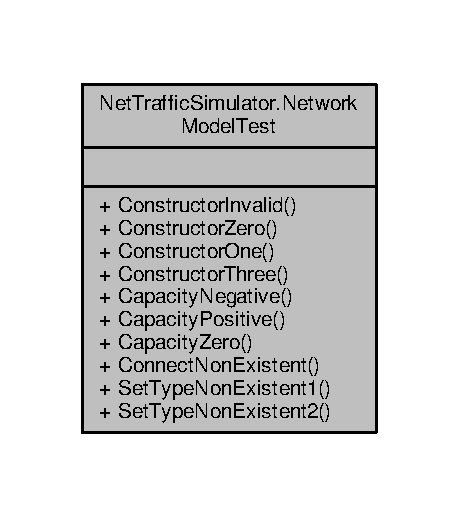
\includegraphics[width=220pt]{classNetTrafficSimulator_1_1NetworkModelTest__coll__graph}
\end{center}
\end{figure}
\subsection*{Public Member Functions}
\begin{DoxyCompactItemize}
\item 
void \hyperlink{classNetTrafficSimulator_1_1NetworkModelTest_afbd7470eb35b97512aa94a2f53163430}{Constructor\-Invalid} ()
\item 
void \hyperlink{classNetTrafficSimulator_1_1NetworkModelTest_a3634f2a5d0e008e7cd8b274615b173ee}{Constructor\-Zero} ()
\item 
void \hyperlink{classNetTrafficSimulator_1_1NetworkModelTest_a6a13d32fefa5e53b7f18e89b2fb8b436}{Constructor\-One} ()
\item 
void \hyperlink{classNetTrafficSimulator_1_1NetworkModelTest_a149aa9eab4b53fb17aa19be215e769b5}{Constructor\-Three} ()
\end{DoxyCompactItemize}


\subsection{Detailed Description}
Test of \hyperlink{classNetTrafficSimulator_1_1NetworkModel}{Network\-Model} class 

\subsection{Member Function Documentation}
\hypertarget{classNetTrafficSimulator_1_1NetworkModelTest_afbd7470eb35b97512aa94a2f53163430}{\index{Net\-Traffic\-Simulator\-::\-Network\-Model\-Test@{Net\-Traffic\-Simulator\-::\-Network\-Model\-Test}!Constructor\-Invalid@{Constructor\-Invalid}}
\index{Constructor\-Invalid@{Constructor\-Invalid}!NetTrafficSimulator::NetworkModelTest@{Net\-Traffic\-Simulator\-::\-Network\-Model\-Test}}
\subsubsection[{Constructor\-Invalid}]{\setlength{\rightskip}{0pt plus 5cm}void Net\-Traffic\-Simulator.\-Network\-Model\-Test.\-Constructor\-Invalid (
\begin{DoxyParamCaption}
{}
\end{DoxyParamCaption}
)\hspace{0.3cm}{\ttfamily [inline]}}}\label{classNetTrafficSimulator_1_1NetworkModelTest_afbd7470eb35b97512aa94a2f53163430}
Try to create model with -\/1 nodes \hypertarget{classNetTrafficSimulator_1_1NetworkModelTest_a6a13d32fefa5e53b7f18e89b2fb8b436}{\index{Net\-Traffic\-Simulator\-::\-Network\-Model\-Test@{Net\-Traffic\-Simulator\-::\-Network\-Model\-Test}!Constructor\-One@{Constructor\-One}}
\index{Constructor\-One@{Constructor\-One}!NetTrafficSimulator::NetworkModelTest@{Net\-Traffic\-Simulator\-::\-Network\-Model\-Test}}
\subsubsection[{Constructor\-One}]{\setlength{\rightskip}{0pt plus 5cm}void Net\-Traffic\-Simulator.\-Network\-Model\-Test.\-Constructor\-One (
\begin{DoxyParamCaption}
{}
\end{DoxyParamCaption}
)\hspace{0.3cm}{\ttfamily [inline]}}}\label{classNetTrafficSimulator_1_1NetworkModelTest_a6a13d32fefa5e53b7f18e89b2fb8b436}
Create model with one node. Assert node is initially unidentified and model invalid, assert node count and connection count. Set node to E\-N\-D\-\_\-\-N\-O\-D\-E type, verify Get\-Node\-Type and Type\mbox{[}0\mbox{]}. Assert model is valid. Print model onto Console. Assert link count. Assert no loop connection \mbox{[}0,0\mbox{]}. Create connection \mbox{[}0,0\mbox{]} and assert model is invalid. Print model onto Console. \hypertarget{classNetTrafficSimulator_1_1NetworkModelTest_a149aa9eab4b53fb17aa19be215e769b5}{\index{Net\-Traffic\-Simulator\-::\-Network\-Model\-Test@{Net\-Traffic\-Simulator\-::\-Network\-Model\-Test}!Constructor\-Three@{Constructor\-Three}}
\index{Constructor\-Three@{Constructor\-Three}!NetTrafficSimulator::NetworkModelTest@{Net\-Traffic\-Simulator\-::\-Network\-Model\-Test}}
\subsubsection[{Constructor\-Three}]{\setlength{\rightskip}{0pt plus 5cm}void Net\-Traffic\-Simulator.\-Network\-Model\-Test.\-Constructor\-Three (
\begin{DoxyParamCaption}
{}
\end{DoxyParamCaption}
)\hspace{0.3cm}{\ttfamily [inline]}}}\label{classNetTrafficSimulator_1_1NetworkModelTest_a149aa9eab4b53fb17aa19be215e769b5}
Create model with 3 elements. Assert all of them are unidentified and model is invalid. Assert node count and all connection counts. Set node types and assert validity. Create connections, print onto Console, assert validity, create invalid connection -\/ assert model not valid, fix and create different invalid connection, assert model not valid \hypertarget{classNetTrafficSimulator_1_1NetworkModelTest_a3634f2a5d0e008e7cd8b274615b173ee}{\index{Net\-Traffic\-Simulator\-::\-Network\-Model\-Test@{Net\-Traffic\-Simulator\-::\-Network\-Model\-Test}!Constructor\-Zero@{Constructor\-Zero}}
\index{Constructor\-Zero@{Constructor\-Zero}!NetTrafficSimulator::NetworkModelTest@{Net\-Traffic\-Simulator\-::\-Network\-Model\-Test}}
\subsubsection[{Constructor\-Zero}]{\setlength{\rightskip}{0pt plus 5cm}void Net\-Traffic\-Simulator.\-Network\-Model\-Test.\-Constructor\-Zero (
\begin{DoxyParamCaption}
{}
\end{DoxyParamCaption}
)\hspace{0.3cm}{\ttfamily [inline]}}}\label{classNetTrafficSimulator_1_1NetworkModelTest_a3634f2a5d0e008e7cd8b274615b173ee}
Create constructor with 0 nodes. Assert node count and validity 

The documentation for this class was generated from the following file\-:\begin{DoxyCompactItemize}
\item 
Net\-Traffic\-Simulator/\-Net\-Traffic\-Simulator/model/\hyperlink{NetworkModelTest_8cs}{Network\-Model\-Test.\-cs}\end{DoxyCompactItemize}

\hypertarget{classNetTrafficSimulator_1_1NetworkNode}{\section{Net\-Traffic\-Simulator.\-Network\-Node Class Reference}
\label{classNetTrafficSimulator_1_1NetworkNode}\index{Net\-Traffic\-Simulator.\-Network\-Node@{Net\-Traffic\-Simulator.\-Network\-Node}}
}


Inheritance diagram for Net\-Traffic\-Simulator.\-Network\-Node\-:
\nopagebreak
\begin{figure}[H]
\begin{center}
\leavevmode
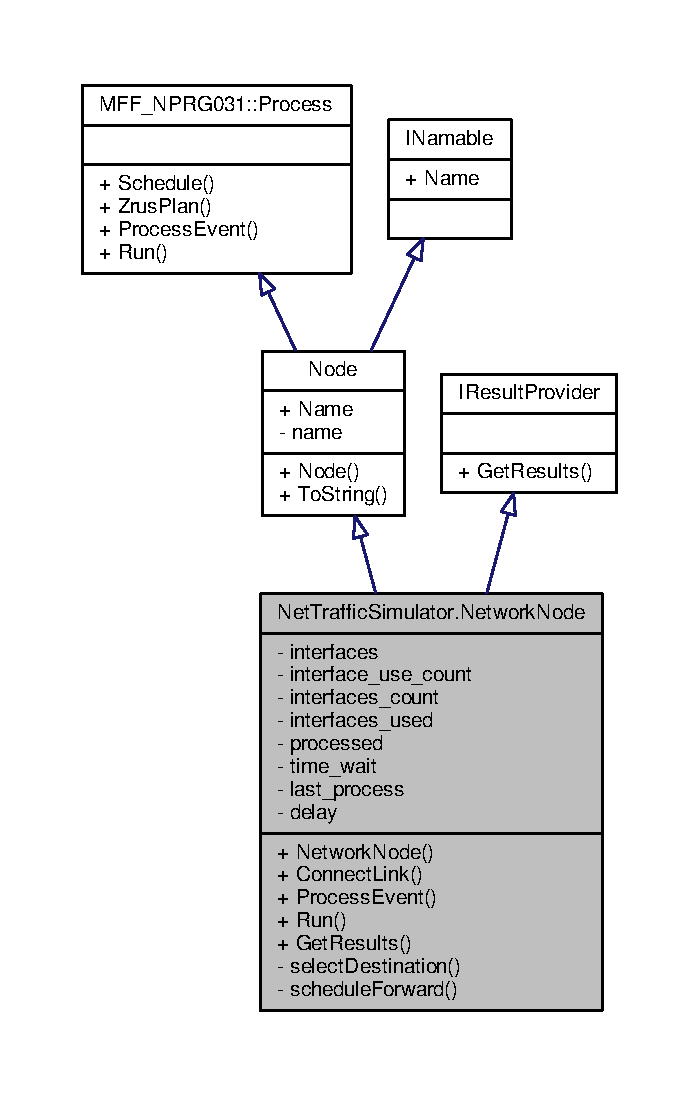
\includegraphics[width=336pt]{classNetTrafficSimulator_1_1NetworkNode__inherit__graph}
\end{center}
\end{figure}


Collaboration diagram for Net\-Traffic\-Simulator.\-Network\-Node\-:
\nopagebreak
\begin{figure}[H]
\begin{center}
\leavevmode
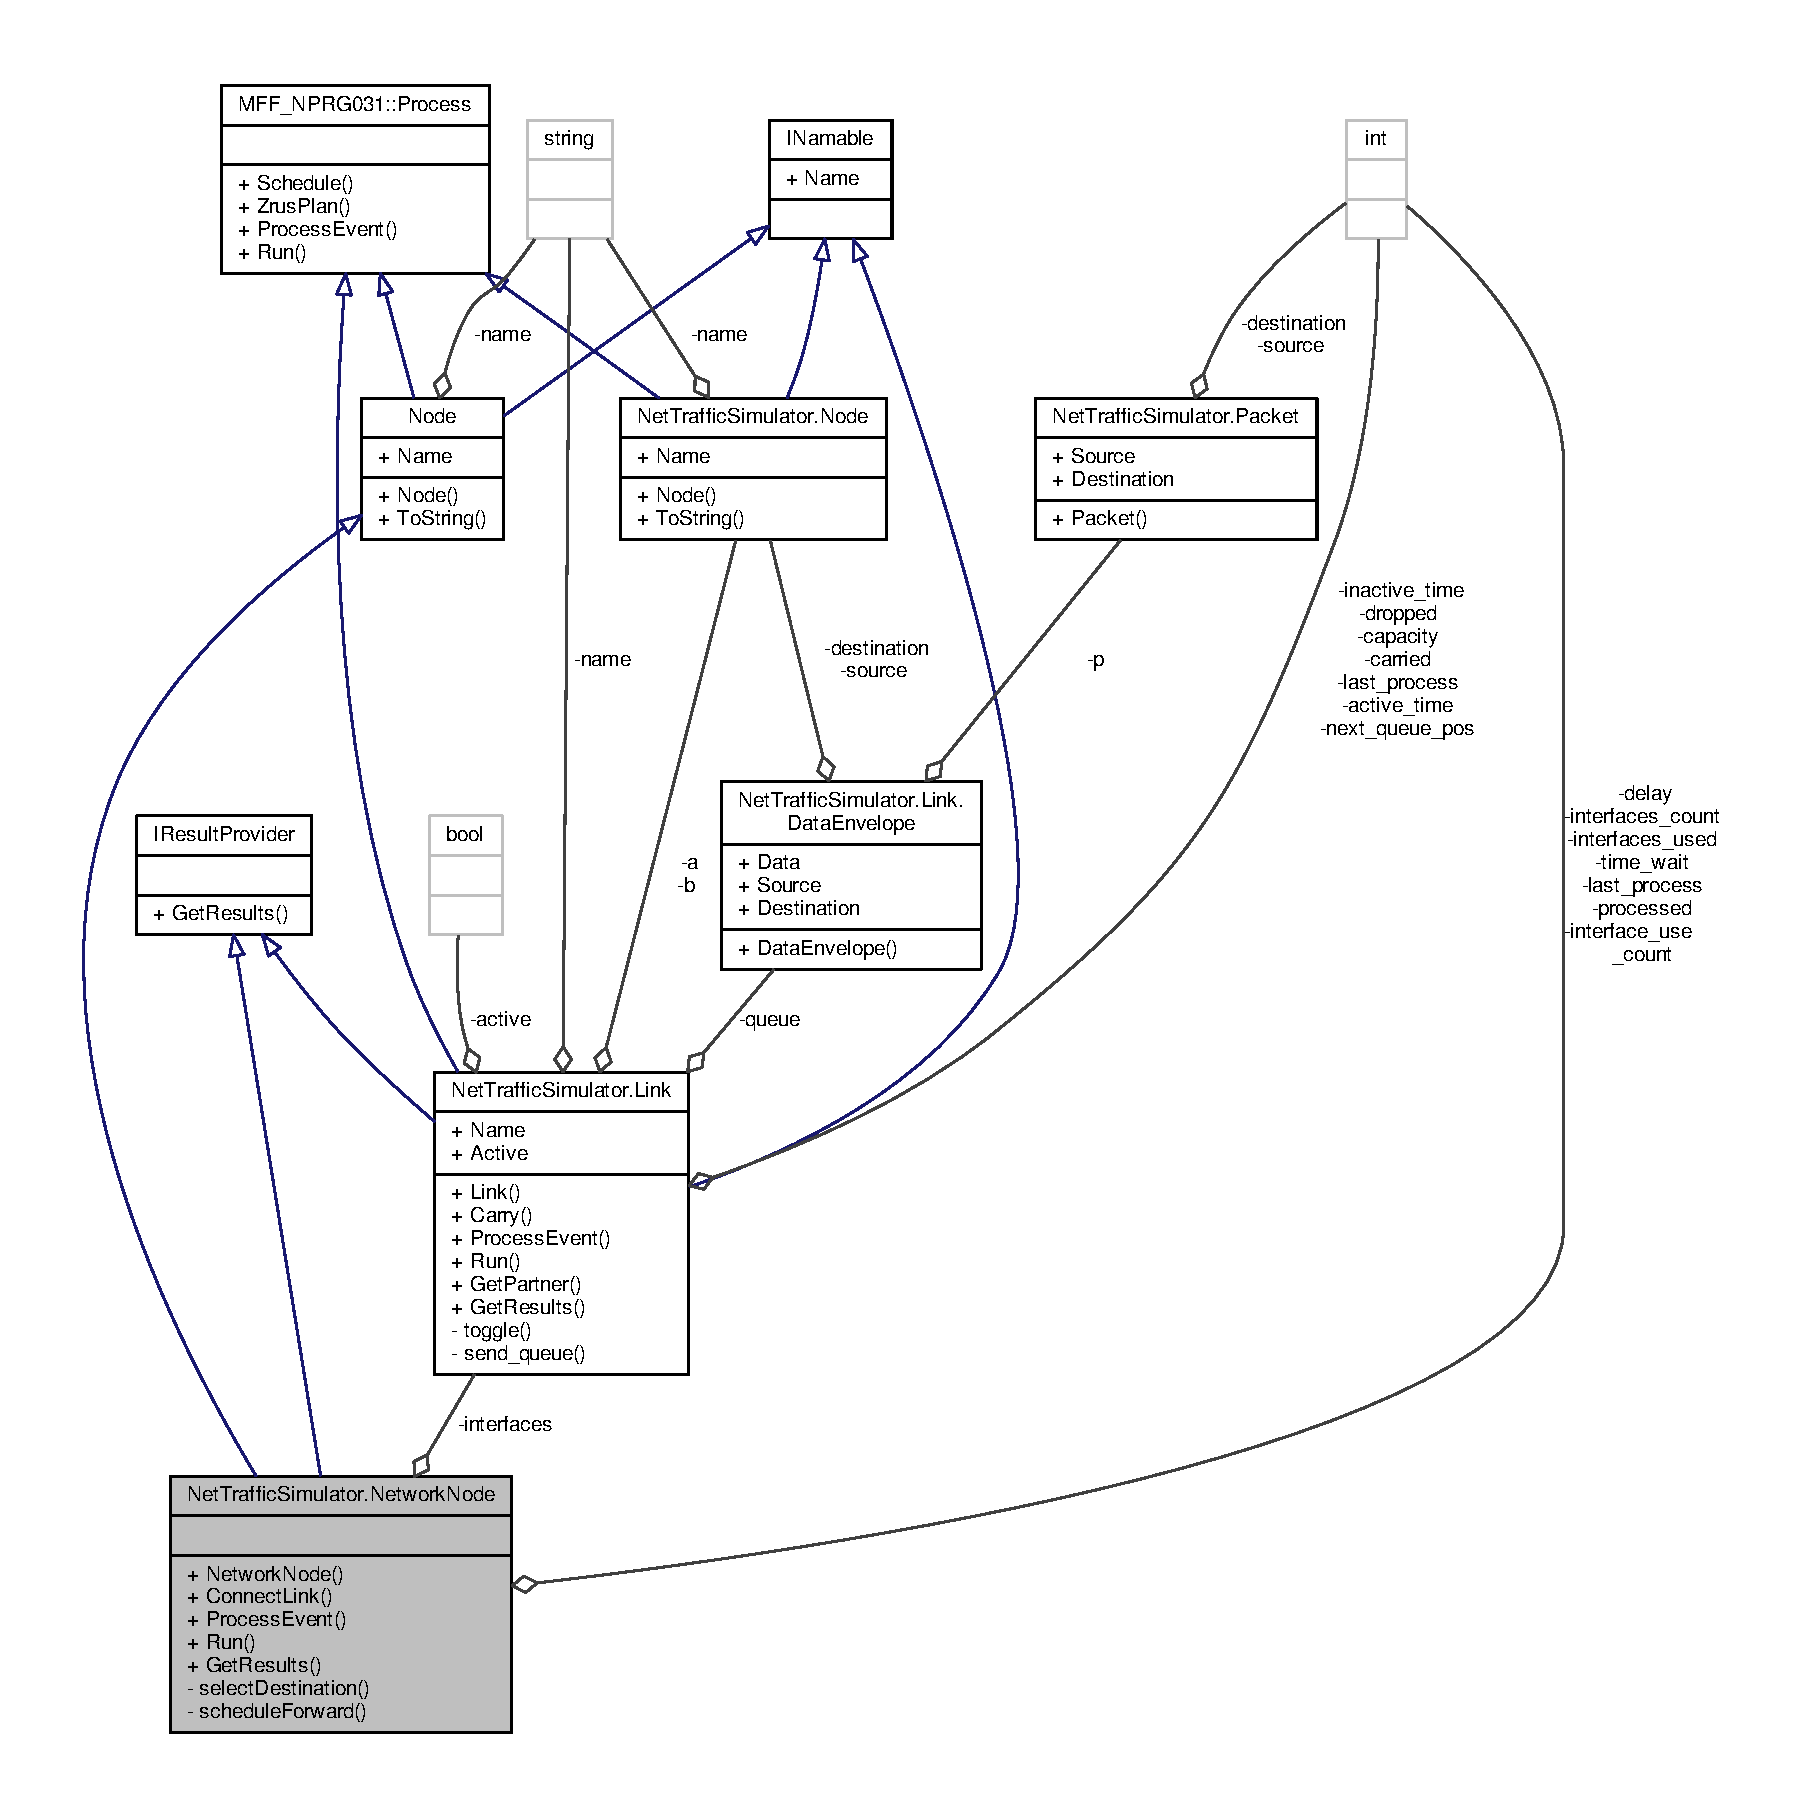
\includegraphics[width=350pt]{classNetTrafficSimulator_1_1NetworkNode__coll__graph}
\end{center}
\end{figure}
\subsection*{Public Member Functions}
\begin{DoxyCompactItemize}
\item 
\hyperlink{classNetTrafficSimulator_1_1NetworkNode_a72e36bcc5eb67db3e7354a01812fcbd9}{Network\-Node} (String \hyperlink{classNetTrafficSimulator_1_1Node_a679d5b6cca77c0cdb46cc98c347d4747}{name}, int \hyperlink{classNetTrafficSimulator_1_1NetworkNode_af9b9d881f9c1b02749716bb12efb5f66}{interfaces\-\_\-count})
\item 
void \hyperlink{classNetTrafficSimulator_1_1NetworkNode_a03e1d48e53fa9405411664e75792b5ec}{Connect\-Link} (\hyperlink{classNetTrafficSimulator_1_1Link}{Link} l)
\item 
override void \hyperlink{classNetTrafficSimulator_1_1NetworkNode_a4a629c1d159d4addef85742089506d20}{Process\-Event} (\hyperlink{classMFF__NPRG031_1_1State}{M\-F\-F\-\_\-\-N\-P\-R\-G031.\-State} state, \hyperlink{classMFF__NPRG031_1_1Model}{M\-F\-F\-\_\-\-N\-P\-R\-G031.\-Model} model)
\item 
override void \hyperlink{classNetTrafficSimulator_1_1NetworkNode_ac4210159f0193e7872d356f40f0b99fe}{Run} (\hyperlink{classMFF__NPRG031_1_1Model}{M\-F\-F\-\_\-\-N\-P\-R\-G031.\-Model} m)
\item 
Dictionary$<$ string, object $>$ \hyperlink{classNetTrafficSimulator_1_1NetworkNode_a7af0bcddea5c043f7e6ff2ac692e09f7}{Get\-Results} (\hyperlink{classMFF__NPRG031_1_1Model}{M\-F\-F\-\_\-\-N\-P\-R\-G031.\-Model} model)
\end{DoxyCompactItemize}
\subsection*{Private Member Functions}
\begin{DoxyCompactItemize}
\item 
\hyperlink{classNetTrafficSimulator_1_1Link}{Link} \hyperlink{classNetTrafficSimulator_1_1NetworkNode_a7a6ad43dc664a81f590da8451f8f3b78}{select\-Destination} (\hyperlink{classNetTrafficSimulator_1_1Packet}{Packet} p)
\item 
void \hyperlink{classNetTrafficSimulator_1_1NetworkNode_a87e1e7c4b163bc96de4ccad302810b2c}{schedule\-Forward} (\hyperlink{classNetTrafficSimulator_1_1Packet}{Packet} p, \hyperlink{classNetTrafficSimulator_1_1Link}{Link} l, \hyperlink{classMFF__NPRG031_1_1Model}{M\-F\-F\-\_\-\-N\-P\-R\-G031.\-Model} model)
\end{DoxyCompactItemize}
\subsection*{Private Attributes}
\begin{DoxyCompactItemize}
\item 
\hyperlink{classNetTrafficSimulator_1_1Link}{Link}\mbox{[}$\,$\mbox{]} \hyperlink{classNetTrafficSimulator_1_1NetworkNode_a88683a8c65aadc6222a5898dcb1735d6}{interfaces}
\item 
int\mbox{[}$\,$\mbox{]} \hyperlink{classNetTrafficSimulator_1_1NetworkNode_a9746a8e4a6c1fc45c1404c9b3d2f8288}{interface\-\_\-use\-\_\-count}
\item 
int \hyperlink{classNetTrafficSimulator_1_1NetworkNode_af9b9d881f9c1b02749716bb12efb5f66}{interfaces\-\_\-count}
\item 
int \hyperlink{classNetTrafficSimulator_1_1NetworkNode_a2a2522005483827b9b7d3b51e7ffc47b}{interfaces\-\_\-used}
\item 
int \hyperlink{classNetTrafficSimulator_1_1NetworkNode_a4d81325b3290fd6521c682c8709b7e65}{processed}
\item 
int \hyperlink{classNetTrafficSimulator_1_1NetworkNode_ad05b46a64426469cee1bc3a0f494e4cb}{time\-\_\-wait}
\item 
int \hyperlink{classNetTrafficSimulator_1_1NetworkNode_afa8095929de9c6ccc20c2d47f8bdee9c}{last\-\_\-process}
\item 
int \hyperlink{classNetTrafficSimulator_1_1NetworkNode_aa31e2256ee97c759bd5f32652a5c00fc}{delay}
\end{DoxyCompactItemize}
\subsection*{Additional Inherited Members}


\subsection{Constructor \& Destructor Documentation}
\hypertarget{classNetTrafficSimulator_1_1NetworkNode_a72e36bcc5eb67db3e7354a01812fcbd9}{\index{Net\-Traffic\-Simulator\-::\-Network\-Node@{Net\-Traffic\-Simulator\-::\-Network\-Node}!Network\-Node@{Network\-Node}}
\index{Network\-Node@{Network\-Node}!NetTrafficSimulator::NetworkNode@{Net\-Traffic\-Simulator\-::\-Network\-Node}}
\subsubsection[{Network\-Node}]{\setlength{\rightskip}{0pt plus 5cm}Net\-Traffic\-Simulator.\-Network\-Node.\-Network\-Node (
\begin{DoxyParamCaption}
\item[{String}]{name, }
\item[{int}]{interfaces\-\_\-count}
\end{DoxyParamCaption}
)\hspace{0.3cm}{\ttfamily [inline]}}}\label{classNetTrafficSimulator_1_1NetworkNode_a72e36bcc5eb67db3e7354a01812fcbd9}
Creates a new network node with given name and interfaces count The delay is set fixed as 1 
\begin{DoxyParams}{Parameters}
{\em name} & Human readable node name \\
\hline
{\em interfaces\-\_\-count} & How many ports does the network node have \\
\hline
\end{DoxyParams}


\subsection{Member Function Documentation}
\hypertarget{classNetTrafficSimulator_1_1NetworkNode_a03e1d48e53fa9405411664e75792b5ec}{\index{Net\-Traffic\-Simulator\-::\-Network\-Node@{Net\-Traffic\-Simulator\-::\-Network\-Node}!Connect\-Link@{Connect\-Link}}
\index{Connect\-Link@{Connect\-Link}!NetTrafficSimulator::NetworkNode@{Net\-Traffic\-Simulator\-::\-Network\-Node}}
\subsubsection[{Connect\-Link}]{\setlength{\rightskip}{0pt plus 5cm}void Net\-Traffic\-Simulator.\-Network\-Node.\-Connect\-Link (
\begin{DoxyParamCaption}
\item[{{\bf Link}}]{l}
\end{DoxyParamCaption}
)\hspace{0.3cm}{\ttfamily [inline]}}}\label{classNetTrafficSimulator_1_1NetworkNode_a03e1d48e53fa9405411664e75792b5ec}
If possible, note a new link in use on first interface available 
\begin{DoxyParams}{Parameters}
{\em l} & \hyperlink{classNetTrafficSimulator_1_1Link}{Link} to connect \\
\hline
\end{DoxyParams}

\begin{DoxyExceptions}{Exceptions}
{\em Argument\-Exception} & if no port is available \\
\hline
\end{DoxyExceptions}
\hypertarget{classNetTrafficSimulator_1_1NetworkNode_a7af0bcddea5c043f7e6ff2ac692e09f7}{\index{Net\-Traffic\-Simulator\-::\-Network\-Node@{Net\-Traffic\-Simulator\-::\-Network\-Node}!Get\-Results@{Get\-Results}}
\index{Get\-Results@{Get\-Results}!NetTrafficSimulator::NetworkNode@{Net\-Traffic\-Simulator\-::\-Network\-Node}}
\subsubsection[{Get\-Results}]{\setlength{\rightskip}{0pt plus 5cm}Dictionary$<$string,object$>$ Net\-Traffic\-Simulator.\-Network\-Node.\-Get\-Results (
\begin{DoxyParamCaption}
\item[{{\bf M\-F\-F\-\_\-\-N\-P\-R\-G031.\-Model}}]{model}
\end{DoxyParamCaption}
)\hspace{0.3cm}{\ttfamily [inline]}}}\label{classNetTrafficSimulator_1_1NetworkNode_a7af0bcddea5c043f7e6ff2ac692e09f7}
Provide results measured during simulation for populating a result model \begin{DoxyReturn}{Returns}
Dictionary, where string is a key representing a human-\/readable description of measured data and object is value measured 
\end{DoxyReturn}


Implements \hyperlink{interfaceNetTrafficSimulator_1_1IResultProvider_ac7053c11f509ba1c2f653cd952b05323}{Net\-Traffic\-Simulator.\-I\-Result\-Provider}.

\hypertarget{classNetTrafficSimulator_1_1NetworkNode_a4a629c1d159d4addef85742089506d20}{\index{Net\-Traffic\-Simulator\-::\-Network\-Node@{Net\-Traffic\-Simulator\-::\-Network\-Node}!Process\-Event@{Process\-Event}}
\index{Process\-Event@{Process\-Event}!NetTrafficSimulator::NetworkNode@{Net\-Traffic\-Simulator\-::\-Network\-Node}}
\subsubsection[{Process\-Event}]{\setlength{\rightskip}{0pt plus 5cm}override void Net\-Traffic\-Simulator.\-Network\-Node.\-Process\-Event (
\begin{DoxyParamCaption}
\item[{{\bf M\-F\-F\-\_\-\-N\-P\-R\-G031.\-State}}]{state, }
\item[{{\bf M\-F\-F\-\_\-\-N\-P\-R\-G031.\-Model}}]{model}
\end{DoxyParamCaption}
)\hspace{0.3cm}{\ttfamily [inline]}, {\ttfamily [virtual]}}}\label{classNetTrafficSimulator_1_1NetworkNode_a4a629c1d159d4addef85742089506d20}
Abstract method Process\-Event for process to react on event hapened 
\begin{DoxyParams}{Parameters}
{\em state} & In what state the process is now \\
\hline
{\em model} & Our simulation model \\
\hline
\end{DoxyParams}


Implements \hyperlink{classMFF__NPRG031_1_1Process_acb58d206e76c177264614d88f1818fdc}{M\-F\-F\-\_\-\-N\-P\-R\-G031.\-Process}.



Here is the call graph for this function\-:\nopagebreak
\begin{figure}[H]
\begin{center}
\leavevmode
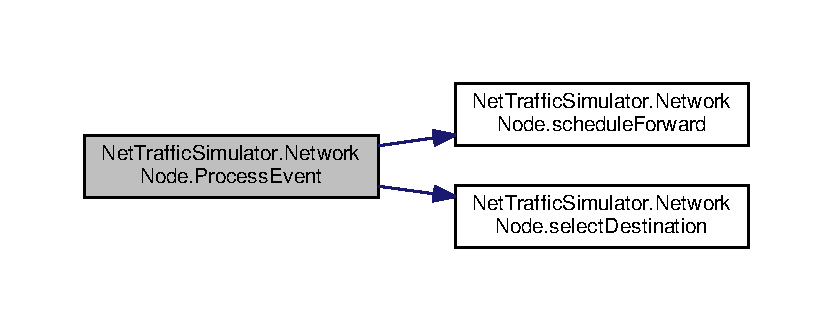
\includegraphics[width=350pt]{classNetTrafficSimulator_1_1NetworkNode_a4a629c1d159d4addef85742089506d20_cgraph}
\end{center}
\end{figure}


\hypertarget{classNetTrafficSimulator_1_1NetworkNode_ac4210159f0193e7872d356f40f0b99fe}{\index{Net\-Traffic\-Simulator\-::\-Network\-Node@{Net\-Traffic\-Simulator\-::\-Network\-Node}!Run@{Run}}
\index{Run@{Run}!NetTrafficSimulator::NetworkNode@{Net\-Traffic\-Simulator\-::\-Network\-Node}}
\subsubsection[{Run}]{\setlength{\rightskip}{0pt plus 5cm}override void Net\-Traffic\-Simulator.\-Network\-Node.\-Run (
\begin{DoxyParamCaption}
\item[{{\bf M\-F\-F\-\_\-\-N\-P\-R\-G031.\-Model}}]{m}
\end{DoxyParamCaption}
)\hspace{0.3cm}{\ttfamily [inline]}, {\ttfamily [virtual]}}}\label{classNetTrafficSimulator_1_1NetworkNode_ac4210159f0193e7872d356f40f0b99fe}
Empty 

Implements \hyperlink{classMFF__NPRG031_1_1Process_ad0e440dee98ba26c59ab22a60ebcafdd}{M\-F\-F\-\_\-\-N\-P\-R\-G031.\-Process}.

\hypertarget{classNetTrafficSimulator_1_1NetworkNode_a87e1e7c4b163bc96de4ccad302810b2c}{\index{Net\-Traffic\-Simulator\-::\-Network\-Node@{Net\-Traffic\-Simulator\-::\-Network\-Node}!schedule\-Forward@{schedule\-Forward}}
\index{schedule\-Forward@{schedule\-Forward}!NetTrafficSimulator::NetworkNode@{Net\-Traffic\-Simulator\-::\-Network\-Node}}
\subsubsection[{schedule\-Forward}]{\setlength{\rightskip}{0pt plus 5cm}void Net\-Traffic\-Simulator.\-Network\-Node.\-schedule\-Forward (
\begin{DoxyParamCaption}
\item[{{\bf Packet}}]{p, }
\item[{{\bf Link}}]{l, }
\item[{{\bf M\-F\-F\-\_\-\-N\-P\-R\-G031.\-Model}}]{model}
\end{DoxyParamCaption}
)\hspace{0.3cm}{\ttfamily [inline]}, {\ttfamily [private]}}}\label{classNetTrafficSimulator_1_1NetworkNode_a87e1e7c4b163bc96de4ccad302810b2c}
Given the packet and the link to use, schedule S\-E\-N\-D for the link with packet included at time T+delay 
\begin{DoxyParams}{Parameters}
{\em p} & \hyperlink{classNetTrafficSimulator_1_1Packet}{Packet} to forward \\
\hline
{\em l} & \hyperlink{classNetTrafficSimulator_1_1Link}{Link} to use (result of select\-Destination) \\
\hline
{\em model} & the Model \\
\hline
\end{DoxyParams}


Here is the caller graph for this function\-:\nopagebreak
\begin{figure}[H]
\begin{center}
\leavevmode
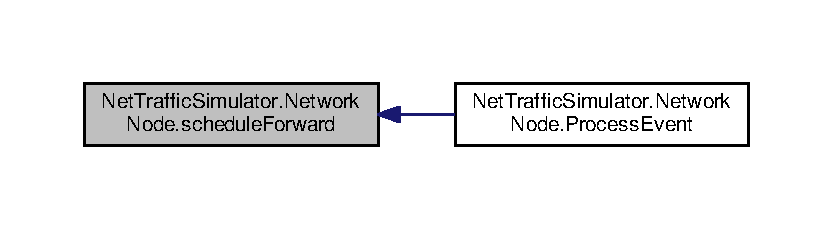
\includegraphics[width=350pt]{classNetTrafficSimulator_1_1NetworkNode_a87e1e7c4b163bc96de4ccad302810b2c_icgraph}
\end{center}
\end{figure}


\hypertarget{classNetTrafficSimulator_1_1NetworkNode_a7a6ad43dc664a81f590da8451f8f3b78}{\index{Net\-Traffic\-Simulator\-::\-Network\-Node@{Net\-Traffic\-Simulator\-::\-Network\-Node}!select\-Destination@{select\-Destination}}
\index{select\-Destination@{select\-Destination}!NetTrafficSimulator::NetworkNode@{Net\-Traffic\-Simulator\-::\-Network\-Node}}
\subsubsection[{select\-Destination}]{\setlength{\rightskip}{0pt plus 5cm}{\bf Link} Net\-Traffic\-Simulator.\-Network\-Node.\-select\-Destination (
\begin{DoxyParamCaption}
\item[{{\bf Packet}}]{p}
\end{DoxyParamCaption}
)\hspace{0.3cm}{\ttfamily [inline]}, {\ttfamily [private]}}}\label{classNetTrafficSimulator_1_1NetworkNode_a7a6ad43dc664a81f590da8451f8f3b78}


Here is the caller graph for this function\-:\nopagebreak
\begin{figure}[H]
\begin{center}
\leavevmode
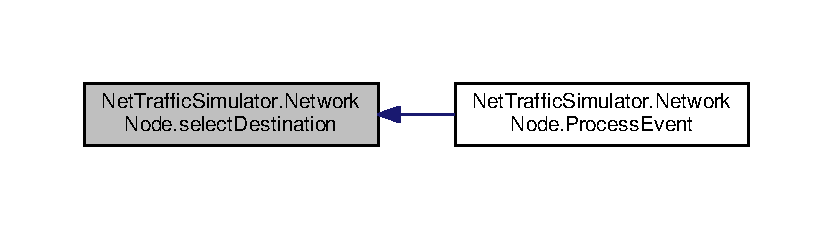
\includegraphics[width=350pt]{classNetTrafficSimulator_1_1NetworkNode_a7a6ad43dc664a81f590da8451f8f3b78_icgraph}
\end{center}
\end{figure}




\subsection{Member Data Documentation}
\hypertarget{classNetTrafficSimulator_1_1NetworkNode_aa31e2256ee97c759bd5f32652a5c00fc}{\index{Net\-Traffic\-Simulator\-::\-Network\-Node@{Net\-Traffic\-Simulator\-::\-Network\-Node}!delay@{delay}}
\index{delay@{delay}!NetTrafficSimulator::NetworkNode@{Net\-Traffic\-Simulator\-::\-Network\-Node}}
\subsubsection[{delay}]{\setlength{\rightskip}{0pt plus 5cm}int Net\-Traffic\-Simulator.\-Network\-Node.\-delay\hspace{0.3cm}{\ttfamily [private]}}}\label{classNetTrafficSimulator_1_1NetworkNode_aa31e2256ee97c759bd5f32652a5c00fc}
\hypertarget{classNetTrafficSimulator_1_1NetworkNode_a9746a8e4a6c1fc45c1404c9b3d2f8288}{\index{Net\-Traffic\-Simulator\-::\-Network\-Node@{Net\-Traffic\-Simulator\-::\-Network\-Node}!interface\-\_\-use\-\_\-count@{interface\-\_\-use\-\_\-count}}
\index{interface\-\_\-use\-\_\-count@{interface\-\_\-use\-\_\-count}!NetTrafficSimulator::NetworkNode@{Net\-Traffic\-Simulator\-::\-Network\-Node}}
\subsubsection[{interface\-\_\-use\-\_\-count}]{\setlength{\rightskip}{0pt plus 5cm}int \mbox{[}$\,$\mbox{]} Net\-Traffic\-Simulator.\-Network\-Node.\-interface\-\_\-use\-\_\-count\hspace{0.3cm}{\ttfamily [private]}}}\label{classNetTrafficSimulator_1_1NetworkNode_a9746a8e4a6c1fc45c1404c9b3d2f8288}
\hypertarget{classNetTrafficSimulator_1_1NetworkNode_a88683a8c65aadc6222a5898dcb1735d6}{\index{Net\-Traffic\-Simulator\-::\-Network\-Node@{Net\-Traffic\-Simulator\-::\-Network\-Node}!interfaces@{interfaces}}
\index{interfaces@{interfaces}!NetTrafficSimulator::NetworkNode@{Net\-Traffic\-Simulator\-::\-Network\-Node}}
\subsubsection[{interfaces}]{\setlength{\rightskip}{0pt plus 5cm}{\bf Link} \mbox{[}$\,$\mbox{]} Net\-Traffic\-Simulator.\-Network\-Node.\-interfaces\hspace{0.3cm}{\ttfamily [private]}}}\label{classNetTrafficSimulator_1_1NetworkNode_a88683a8c65aadc6222a5898dcb1735d6}
\hypertarget{classNetTrafficSimulator_1_1NetworkNode_af9b9d881f9c1b02749716bb12efb5f66}{\index{Net\-Traffic\-Simulator\-::\-Network\-Node@{Net\-Traffic\-Simulator\-::\-Network\-Node}!interfaces\-\_\-count@{interfaces\-\_\-count}}
\index{interfaces\-\_\-count@{interfaces\-\_\-count}!NetTrafficSimulator::NetworkNode@{Net\-Traffic\-Simulator\-::\-Network\-Node}}
\subsubsection[{interfaces\-\_\-count}]{\setlength{\rightskip}{0pt plus 5cm}int Net\-Traffic\-Simulator.\-Network\-Node.\-interfaces\-\_\-count\hspace{0.3cm}{\ttfamily [private]}}}\label{classNetTrafficSimulator_1_1NetworkNode_af9b9d881f9c1b02749716bb12efb5f66}
\hypertarget{classNetTrafficSimulator_1_1NetworkNode_a2a2522005483827b9b7d3b51e7ffc47b}{\index{Net\-Traffic\-Simulator\-::\-Network\-Node@{Net\-Traffic\-Simulator\-::\-Network\-Node}!interfaces\-\_\-used@{interfaces\-\_\-used}}
\index{interfaces\-\_\-used@{interfaces\-\_\-used}!NetTrafficSimulator::NetworkNode@{Net\-Traffic\-Simulator\-::\-Network\-Node}}
\subsubsection[{interfaces\-\_\-used}]{\setlength{\rightskip}{0pt plus 5cm}int Net\-Traffic\-Simulator.\-Network\-Node.\-interfaces\-\_\-used\hspace{0.3cm}{\ttfamily [private]}}}\label{classNetTrafficSimulator_1_1NetworkNode_a2a2522005483827b9b7d3b51e7ffc47b}
\hypertarget{classNetTrafficSimulator_1_1NetworkNode_afa8095929de9c6ccc20c2d47f8bdee9c}{\index{Net\-Traffic\-Simulator\-::\-Network\-Node@{Net\-Traffic\-Simulator\-::\-Network\-Node}!last\-\_\-process@{last\-\_\-process}}
\index{last\-\_\-process@{last\-\_\-process}!NetTrafficSimulator::NetworkNode@{Net\-Traffic\-Simulator\-::\-Network\-Node}}
\subsubsection[{last\-\_\-process}]{\setlength{\rightskip}{0pt plus 5cm}int Net\-Traffic\-Simulator.\-Network\-Node.\-last\-\_\-process\hspace{0.3cm}{\ttfamily [private]}}}\label{classNetTrafficSimulator_1_1NetworkNode_afa8095929de9c6ccc20c2d47f8bdee9c}
\hypertarget{classNetTrafficSimulator_1_1NetworkNode_a4d81325b3290fd6521c682c8709b7e65}{\index{Net\-Traffic\-Simulator\-::\-Network\-Node@{Net\-Traffic\-Simulator\-::\-Network\-Node}!processed@{processed}}
\index{processed@{processed}!NetTrafficSimulator::NetworkNode@{Net\-Traffic\-Simulator\-::\-Network\-Node}}
\subsubsection[{processed}]{\setlength{\rightskip}{0pt plus 5cm}int Net\-Traffic\-Simulator.\-Network\-Node.\-processed\hspace{0.3cm}{\ttfamily [private]}}}\label{classNetTrafficSimulator_1_1NetworkNode_a4d81325b3290fd6521c682c8709b7e65}
\hypertarget{classNetTrafficSimulator_1_1NetworkNode_ad05b46a64426469cee1bc3a0f494e4cb}{\index{Net\-Traffic\-Simulator\-::\-Network\-Node@{Net\-Traffic\-Simulator\-::\-Network\-Node}!time\-\_\-wait@{time\-\_\-wait}}
\index{time\-\_\-wait@{time\-\_\-wait}!NetTrafficSimulator::NetworkNode@{Net\-Traffic\-Simulator\-::\-Network\-Node}}
\subsubsection[{time\-\_\-wait}]{\setlength{\rightskip}{0pt plus 5cm}int Net\-Traffic\-Simulator.\-Network\-Node.\-time\-\_\-wait\hspace{0.3cm}{\ttfamily [private]}}}\label{classNetTrafficSimulator_1_1NetworkNode_ad05b46a64426469cee1bc3a0f494e4cb}


The documentation for this class was generated from the following file\-:\begin{DoxyCompactItemize}
\item 
Net\-Traffic\-Simulator/\-Net\-Traffic\-Simulator/framework/extension/\hyperlink{NetworkNode_8cs}{Network\-Node.\-cs}\end{DoxyCompactItemize}

\hypertarget{classNetTrafficSimulator_1_1Node}{\section{Net\-Traffic\-Simulator.\-Node Class Reference}
\label{classNetTrafficSimulator_1_1Node}\index{Net\-Traffic\-Simulator.\-Node@{Net\-Traffic\-Simulator.\-Node}}
}


Inheritance diagram for Net\-Traffic\-Simulator.\-Node\-:
\nopagebreak
\begin{figure}[H]
\begin{center}
\leavevmode
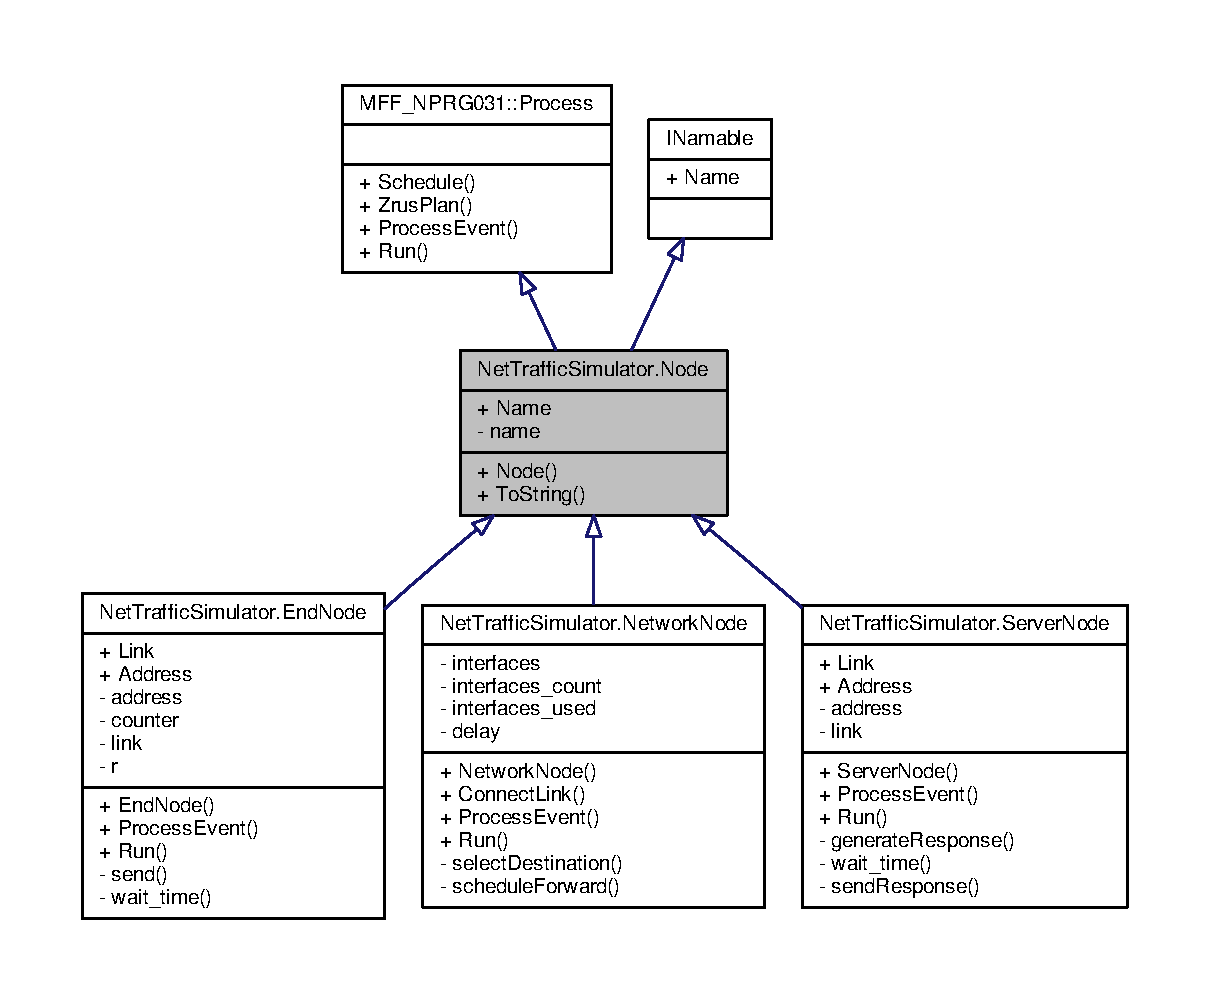
\includegraphics[width=350pt]{classNetTrafficSimulator_1_1Node__inherit__graph}
\end{center}
\end{figure}


Collaboration diagram for Net\-Traffic\-Simulator.\-Node\-:\nopagebreak
\begin{figure}[H]
\begin{center}
\leavevmode
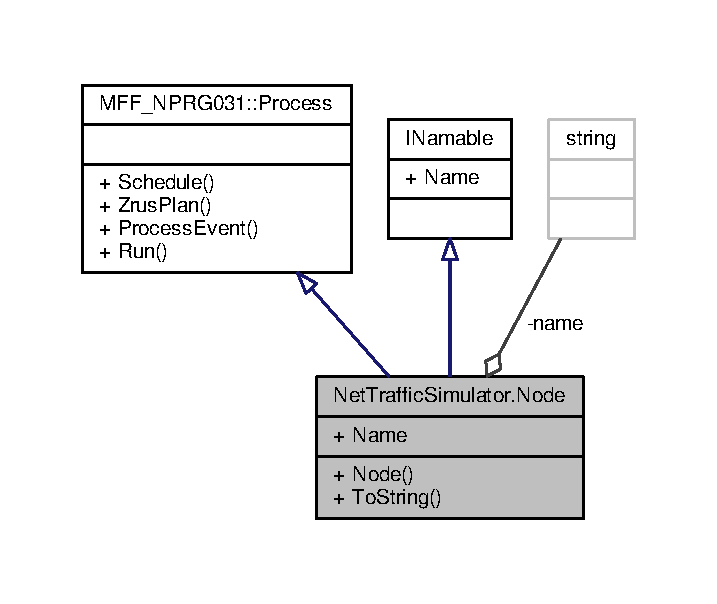
\includegraphics[width=344pt]{classNetTrafficSimulator_1_1Node__coll__graph}
\end{center}
\end{figure}
\subsection*{Public Member Functions}
\begin{DoxyCompactItemize}
\item 
\hyperlink{classNetTrafficSimulator_1_1Node_af6e132b65905bc9a19588da0e9d5c6c5}{Node} (string \hyperlink{classNetTrafficSimulator_1_1Node_a679d5b6cca77c0cdb46cc98c347d4747}{name})
\item 
override string \hyperlink{classNetTrafficSimulator_1_1Node_a870d79397fee5f2d8d5f59c4bfeaa72c}{To\-String} ()
\end{DoxyCompactItemize}
\subsection*{Properties}
\begin{DoxyCompactItemize}
\item 
string \hyperlink{classNetTrafficSimulator_1_1Node_a326ffcdc9c20fd88efe21495a525a57e}{Name}\hspace{0.3cm}{\ttfamily  \mbox{[}get\mbox{]}}
\end{DoxyCompactItemize}
\subsection*{Private Attributes}
\begin{DoxyCompactItemize}
\item 
string \hyperlink{classNetTrafficSimulator_1_1Node_a679d5b6cca77c0cdb46cc98c347d4747}{name}
\end{DoxyCompactItemize}


\subsection{Constructor \& Destructor Documentation}
\hypertarget{classNetTrafficSimulator_1_1Node_af6e132b65905bc9a19588da0e9d5c6c5}{\index{Net\-Traffic\-Simulator\-::\-Node@{Net\-Traffic\-Simulator\-::\-Node}!Node@{Node}}
\index{Node@{Node}!NetTrafficSimulator::Node@{Net\-Traffic\-Simulator\-::\-Node}}
\subsubsection[{Node}]{\setlength{\rightskip}{0pt plus 5cm}Net\-Traffic\-Simulator.\-Node.\-Node (
\begin{DoxyParamCaption}
\item[{string}]{name}
\end{DoxyParamCaption}
)\hspace{0.3cm}{\ttfamily [inline]}}}\label{classNetTrafficSimulator_1_1Node_af6e132b65905bc9a19588da0e9d5c6c5}
Create a new node with the human readable name specified 
\begin{DoxyParams}{Parameters}
{\em name} & human readable name \\
\hline
\end{DoxyParams}


\subsection{Member Function Documentation}
\hypertarget{classNetTrafficSimulator_1_1Node_a870d79397fee5f2d8d5f59c4bfeaa72c}{\index{Net\-Traffic\-Simulator\-::\-Node@{Net\-Traffic\-Simulator\-::\-Node}!To\-String@{To\-String}}
\index{To\-String@{To\-String}!NetTrafficSimulator::Node@{Net\-Traffic\-Simulator\-::\-Node}}
\subsubsection[{To\-String}]{\setlength{\rightskip}{0pt plus 5cm}override string Net\-Traffic\-Simulator.\-Node.\-To\-String (
\begin{DoxyParamCaption}
{}
\end{DoxyParamCaption}
)\hspace{0.3cm}{\ttfamily [inline]}}}\label{classNetTrafficSimulator_1_1Node_a870d79397fee5f2d8d5f59c4bfeaa72c}
String representation of a node is it's name \begin{DoxyReturn}{Returns}
the node name 
\end{DoxyReturn}


\subsection{Member Data Documentation}
\hypertarget{classNetTrafficSimulator_1_1Node_a679d5b6cca77c0cdb46cc98c347d4747}{\index{Net\-Traffic\-Simulator\-::\-Node@{Net\-Traffic\-Simulator\-::\-Node}!name@{name}}
\index{name@{name}!NetTrafficSimulator::Node@{Net\-Traffic\-Simulator\-::\-Node}}
\subsubsection[{name}]{\setlength{\rightskip}{0pt plus 5cm}string Net\-Traffic\-Simulator.\-Node.\-name\hspace{0.3cm}{\ttfamily [private]}}}\label{classNetTrafficSimulator_1_1Node_a679d5b6cca77c0cdb46cc98c347d4747}


\subsection{Property Documentation}
\hypertarget{classNetTrafficSimulator_1_1Node_a326ffcdc9c20fd88efe21495a525a57e}{\index{Net\-Traffic\-Simulator\-::\-Node@{Net\-Traffic\-Simulator\-::\-Node}!Name@{Name}}
\index{Name@{Name}!NetTrafficSimulator::Node@{Net\-Traffic\-Simulator\-::\-Node}}
\subsubsection[{Name}]{\setlength{\rightskip}{0pt plus 5cm}string Net\-Traffic\-Simulator.\-Node.\-Name\hspace{0.3cm}{\ttfamily [get]}}}\label{classNetTrafficSimulator_1_1Node_a326ffcdc9c20fd88efe21495a525a57e}
Human readable name of the node \begin{DoxyReturn}{Returns}
the node name 
\end{DoxyReturn}


The documentation for this class was generated from the following file\-:\begin{DoxyCompactItemize}
\item 
Net\-Traffic\-Simulator/\-Net\-Traffic\-Simulator/framework/extension/\hyperlink{Node_8cs}{Node.\-cs}\end{DoxyCompactItemize}

\hypertarget{classNetTrafficSimulator_1_1Packet}{\section{Net\-Traffic\-Simulator.\-Packet Class Reference}
\label{classNetTrafficSimulator_1_1Packet}\index{Net\-Traffic\-Simulator.\-Packet@{Net\-Traffic\-Simulator.\-Packet}}
}


Collaboration diagram for Net\-Traffic\-Simulator.\-Packet\-:\nopagebreak
\begin{figure}[H]
\begin{center}
\leavevmode
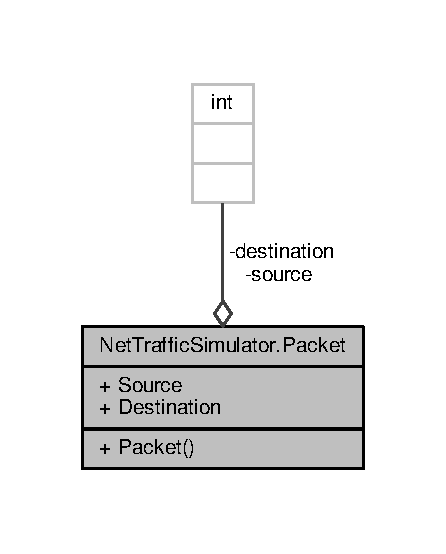
\includegraphics[width=214pt]{classNetTrafficSimulator_1_1Packet__coll__graph}
\end{center}
\end{figure}
\subsection*{Public Member Functions}
\begin{DoxyCompactItemize}
\item 
\hyperlink{classNetTrafficSimulator_1_1Packet_a7f873b329bd79faac2022a2ca4f77ed9}{Packet} (int \hyperlink{classNetTrafficSimulator_1_1Packet_a14e22dc3d532950074fe557df6b05324}{source}, int \hyperlink{classNetTrafficSimulator_1_1Packet_abb858df4db6996ea17200fb0369a7b2c}{destination})
\end{DoxyCompactItemize}
\subsection*{Properties}
\begin{DoxyCompactItemize}
\item 
int \hyperlink{classNetTrafficSimulator_1_1Packet_aa1bbb33d4ac2bab95590f51831d9cff8}{Source}\hspace{0.3cm}{\ttfamily  \mbox{[}get\mbox{]}}
\item 
int \hyperlink{classNetTrafficSimulator_1_1Packet_a4b9f5194a86e8ede7235533e5562f3cc}{Destination}\hspace{0.3cm}{\ttfamily  \mbox{[}get\mbox{]}}
\end{DoxyCompactItemize}
\subsection*{Private Attributes}
\begin{DoxyCompactItemize}
\item 
readonly int \hyperlink{classNetTrafficSimulator_1_1Packet_a14e22dc3d532950074fe557df6b05324}{source}
\item 
readonly int \hyperlink{classNetTrafficSimulator_1_1Packet_abb858df4db6996ea17200fb0369a7b2c}{destination}
\end{DoxyCompactItemize}


\subsection{Constructor \& Destructor Documentation}
\hypertarget{classNetTrafficSimulator_1_1Packet_a7f873b329bd79faac2022a2ca4f77ed9}{\index{Net\-Traffic\-Simulator\-::\-Packet@{Net\-Traffic\-Simulator\-::\-Packet}!Packet@{Packet}}
\index{Packet@{Packet}!NetTrafficSimulator::Packet@{Net\-Traffic\-Simulator\-::\-Packet}}
\subsubsection[{Packet}]{\setlength{\rightskip}{0pt plus 5cm}Net\-Traffic\-Simulator.\-Packet.\-Packet (
\begin{DoxyParamCaption}
\item[{int}]{source, }
\item[{int}]{destination}
\end{DoxyParamCaption}
)\hspace{0.3cm}{\ttfamily [inline]}}}\label{classNetTrafficSimulator_1_1Packet_a7f873b329bd79faac2022a2ca4f77ed9}
Creates a packet to travel from the source address specified to the destination address specified 
\begin{DoxyParams}{Parameters}
{\em source} & address of the source node \\
\hline
{\em destination} & address of the destination node \\
\hline
\end{DoxyParams}


\subsection{Member Data Documentation}
\hypertarget{classNetTrafficSimulator_1_1Packet_abb858df4db6996ea17200fb0369a7b2c}{\index{Net\-Traffic\-Simulator\-::\-Packet@{Net\-Traffic\-Simulator\-::\-Packet}!destination@{destination}}
\index{destination@{destination}!NetTrafficSimulator::Packet@{Net\-Traffic\-Simulator\-::\-Packet}}
\subsubsection[{destination}]{\setlength{\rightskip}{0pt plus 5cm}readonly int Net\-Traffic\-Simulator.\-Packet.\-destination\hspace{0.3cm}{\ttfamily [private]}}}\label{classNetTrafficSimulator_1_1Packet_abb858df4db6996ea17200fb0369a7b2c}
\hypertarget{classNetTrafficSimulator_1_1Packet_a14e22dc3d532950074fe557df6b05324}{\index{Net\-Traffic\-Simulator\-::\-Packet@{Net\-Traffic\-Simulator\-::\-Packet}!source@{source}}
\index{source@{source}!NetTrafficSimulator::Packet@{Net\-Traffic\-Simulator\-::\-Packet}}
\subsubsection[{source}]{\setlength{\rightskip}{0pt plus 5cm}readonly int Net\-Traffic\-Simulator.\-Packet.\-source\hspace{0.3cm}{\ttfamily [private]}}}\label{classNetTrafficSimulator_1_1Packet_a14e22dc3d532950074fe557df6b05324}


\subsection{Property Documentation}
\hypertarget{classNetTrafficSimulator_1_1Packet_a4b9f5194a86e8ede7235533e5562f3cc}{\index{Net\-Traffic\-Simulator\-::\-Packet@{Net\-Traffic\-Simulator\-::\-Packet}!Destination@{Destination}}
\index{Destination@{Destination}!NetTrafficSimulator::Packet@{Net\-Traffic\-Simulator\-::\-Packet}}
\subsubsection[{Destination}]{\setlength{\rightskip}{0pt plus 5cm}int Net\-Traffic\-Simulator.\-Packet.\-Destination\hspace{0.3cm}{\ttfamily [get]}}}\label{classNetTrafficSimulator_1_1Packet_a4b9f5194a86e8ede7235533e5562f3cc}
Address of the destination node \hypertarget{classNetTrafficSimulator_1_1Packet_aa1bbb33d4ac2bab95590f51831d9cff8}{\index{Net\-Traffic\-Simulator\-::\-Packet@{Net\-Traffic\-Simulator\-::\-Packet}!Source@{Source}}
\index{Source@{Source}!NetTrafficSimulator::Packet@{Net\-Traffic\-Simulator\-::\-Packet}}
\subsubsection[{Source}]{\setlength{\rightskip}{0pt plus 5cm}int Net\-Traffic\-Simulator.\-Packet.\-Source\hspace{0.3cm}{\ttfamily [get]}}}\label{classNetTrafficSimulator_1_1Packet_aa1bbb33d4ac2bab95590f51831d9cff8}
Address of the source node 

The documentation for this class was generated from the following file\-:\begin{DoxyCompactItemize}
\item 
Net\-Traffic\-Simulator/\-Net\-Traffic\-Simulator/framework/extension/\hyperlink{Packet_8cs}{Packet.\-cs}\end{DoxyCompactItemize}

\hypertarget{classMFF__NPRG031_1_1Process}{\section{M\-F\-F\-\_\-\-N\-P\-R\-G031.\-Process Class Reference}
\label{classMFF__NPRG031_1_1Process}\index{M\-F\-F\-\_\-\-N\-P\-R\-G031.\-Process@{M\-F\-F\-\_\-\-N\-P\-R\-G031.\-Process}}
}


Inheritance diagram for M\-F\-F\-\_\-\-N\-P\-R\-G031.\-Process\-:\nopagebreak
\begin{figure}[H]
\begin{center}
\leavevmode
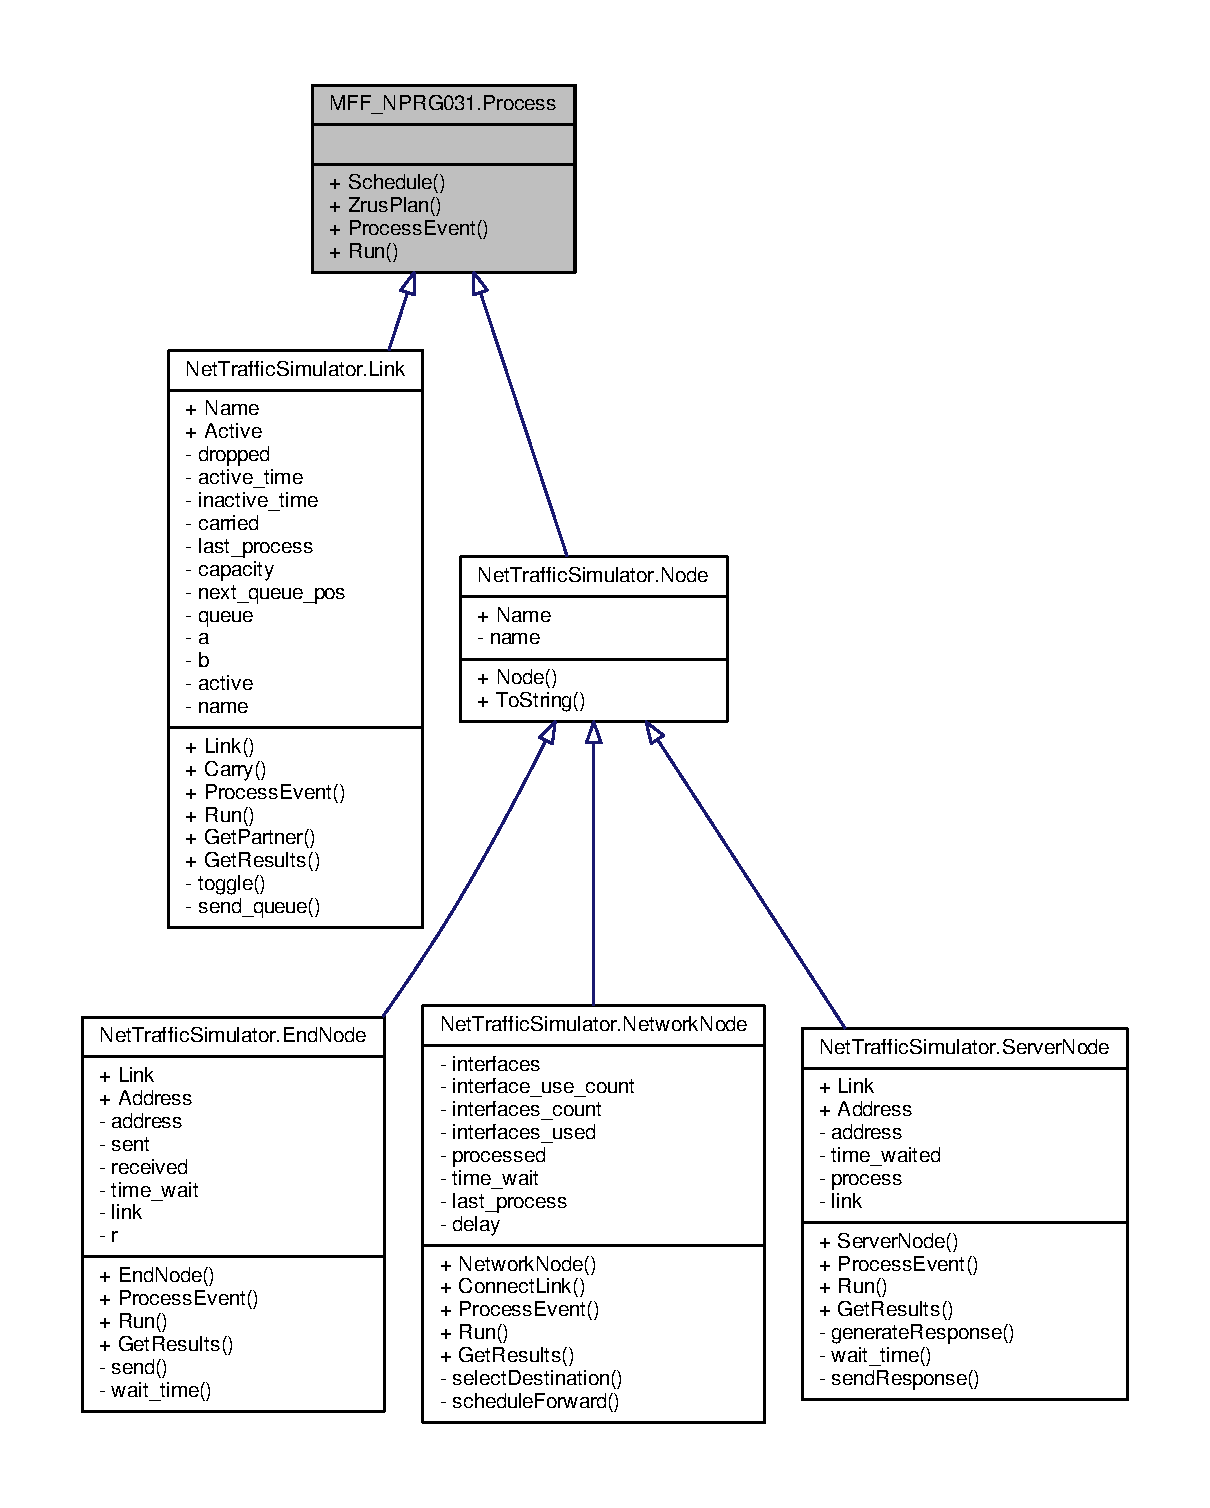
\includegraphics[width=350pt]{classMFF__NPRG031_1_1Process__inherit__graph}
\end{center}
\end{figure}


Collaboration diagram for M\-F\-F\-\_\-\-N\-P\-R\-G031.\-Process\-:\nopagebreak
\begin{figure}[H]
\begin{center}
\leavevmode
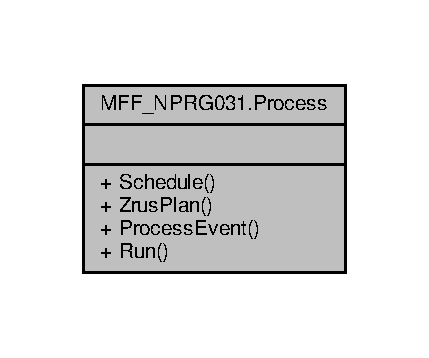
\includegraphics[width=206pt]{classMFF__NPRG031_1_1Process__coll__graph}
\end{center}
\end{figure}
\subsection*{Public Member Functions}
\begin{DoxyCompactItemize}
\item 
void \hyperlink{classMFF__NPRG031_1_1Process_a081e6d0ac9eccaa6b29ea1e2b0586444}{Schedule} (\hyperlink{classMFF__NPRG031_1_1Calendar}{Calendar} calendar, \hyperlink{classMFF__NPRG031_1_1State}{State} what, int when)
\item 
void \hyperlink{classMFF__NPRG031_1_1Process_a48e9c06dfa643a68827557d30d491b0d}{Zrus\-Plan} (\hyperlink{classMFF__NPRG031_1_1Calendar}{Calendar} calendar)
\item 
abstract void \hyperlink{classMFF__NPRG031_1_1Process_acb58d206e76c177264614d88f1818fdc}{Process\-Event} (\hyperlink{classMFF__NPRG031_1_1State}{State} state, \hyperlink{classMFF__NPRG031_1_1Model}{Model} model)
\item 
abstract void \hyperlink{classMFF__NPRG031_1_1Process_ad0e440dee98ba26c59ab22a60ebcafdd}{Run} (\hyperlink{classMFF__NPRG031_1_1Model}{Model} m)
\end{DoxyCompactItemize}


\subsection{Detailed Description}
Abstract process of discrete simulation 

\subsection{Member Function Documentation}
\hypertarget{classMFF__NPRG031_1_1Process_acb58d206e76c177264614d88f1818fdc}{\index{M\-F\-F\-\_\-\-N\-P\-R\-G031\-::\-Process@{M\-F\-F\-\_\-\-N\-P\-R\-G031\-::\-Process}!Process\-Event@{Process\-Event}}
\index{Process\-Event@{Process\-Event}!MFF_NPRG031::Process@{M\-F\-F\-\_\-\-N\-P\-R\-G031\-::\-Process}}
\subsubsection[{Process\-Event}]{\setlength{\rightskip}{0pt plus 5cm}abstract void M\-F\-F\-\_\-\-N\-P\-R\-G031.\-Process.\-Process\-Event (
\begin{DoxyParamCaption}
\item[{{\bf State}}]{state, }
\item[{{\bf Model}}]{model}
\end{DoxyParamCaption}
)\hspace{0.3cm}{\ttfamily [pure virtual]}}}\label{classMFF__NPRG031_1_1Process_acb58d206e76c177264614d88f1818fdc}
Abstract method Process\-Event for process to react on event hapened 
\begin{DoxyParams}{Parameters}
{\em state} & In what state the process is now \\
\hline
{\em model} & Our simulation model \\
\hline
\end{DoxyParams}


Implemented in \hyperlink{classNetTrafficSimulator_1_1Link_a953900c6d1064af45c99b9533eadeafe}{Net\-Traffic\-Simulator.\-Link}, \hyperlink{classNetTrafficSimulator_1_1EndNode_a54624ab4b68ccc8c938905ac3e906623}{Net\-Traffic\-Simulator.\-End\-Node}, \hyperlink{classNetTrafficSimulator_1_1NetworkNode_a4a629c1d159d4addef85742089506d20}{Net\-Traffic\-Simulator.\-Network\-Node}, and \hyperlink{classNetTrafficSimulator_1_1ServerNode_ab309ebda509474d7a7f14b60955e5f98}{Net\-Traffic\-Simulator.\-Server\-Node}.

\hypertarget{classMFF__NPRG031_1_1Process_ad0e440dee98ba26c59ab22a60ebcafdd}{\index{M\-F\-F\-\_\-\-N\-P\-R\-G031\-::\-Process@{M\-F\-F\-\_\-\-N\-P\-R\-G031\-::\-Process}!Run@{Run}}
\index{Run@{Run}!MFF_NPRG031::Process@{M\-F\-F\-\_\-\-N\-P\-R\-G031\-::\-Process}}
\subsubsection[{Run}]{\setlength{\rightskip}{0pt plus 5cm}abstract void M\-F\-F\-\_\-\-N\-P\-R\-G031.\-Process.\-Run (
\begin{DoxyParamCaption}
\item[{{\bf Model}}]{m}
\end{DoxyParamCaption}
)\hspace{0.3cm}{\ttfamily [pure virtual]}}}\label{classMFF__NPRG031_1_1Process_ad0e440dee98ba26c59ab22a60ebcafdd}
Initial set up 
\begin{DoxyParams}{Parameters}
{\em m} & \hyperlink{classMFF__NPRG031_1_1Model}{Model} given \\
\hline
\end{DoxyParams}


Implemented in \hyperlink{classNetTrafficSimulator_1_1Link_a654d0221ce7490d08ad40a70887b80c8}{Net\-Traffic\-Simulator.\-Link}, \hyperlink{classNetTrafficSimulator_1_1EndNode_ad672744610489948d0a8126a84a1aab6}{Net\-Traffic\-Simulator.\-End\-Node}, \hyperlink{classNetTrafficSimulator_1_1NetworkNode_ac4210159f0193e7872d356f40f0b99fe}{Net\-Traffic\-Simulator.\-Network\-Node}, and \hyperlink{classNetTrafficSimulator_1_1ServerNode_aec78a48eea4006df1b4bce59ef17fbf7}{Net\-Traffic\-Simulator.\-Server\-Node}.

\hypertarget{classMFF__NPRG031_1_1Process_a081e6d0ac9eccaa6b29ea1e2b0586444}{\index{M\-F\-F\-\_\-\-N\-P\-R\-G031\-::\-Process@{M\-F\-F\-\_\-\-N\-P\-R\-G031\-::\-Process}!Schedule@{Schedule}}
\index{Schedule@{Schedule}!MFF_NPRG031::Process@{M\-F\-F\-\_\-\-N\-P\-R\-G031\-::\-Process}}
\subsubsection[{Schedule}]{\setlength{\rightskip}{0pt plus 5cm}void M\-F\-F\-\_\-\-N\-P\-R\-G031.\-Process.\-Schedule (
\begin{DoxyParamCaption}
\item[{{\bf Calendar}}]{calendar, }
\item[{{\bf State}}]{what, }
\item[{int}]{when}
\end{DoxyParamCaption}
)\hspace{0.3cm}{\ttfamily [inline]}}}\label{classMFF__NPRG031_1_1Process_a081e6d0ac9eccaa6b29ea1e2b0586444}
Schedule an event to happen in future 
\begin{DoxyParams}{Parameters}
{\em calendar} & \hyperlink{classMFF__NPRG031_1_1Calendar}{Calendar} to schedule the event \\
\hline
{\em what} & In what state the process will be \\
\hline
{\em when} & When the event is to happen \\
\hline
\end{DoxyParams}
\hypertarget{classMFF__NPRG031_1_1Process_a48e9c06dfa643a68827557d30d491b0d}{\index{M\-F\-F\-\_\-\-N\-P\-R\-G031\-::\-Process@{M\-F\-F\-\_\-\-N\-P\-R\-G031\-::\-Process}!Zrus\-Plan@{Zrus\-Plan}}
\index{Zrus\-Plan@{Zrus\-Plan}!MFF_NPRG031::Process@{M\-F\-F\-\_\-\-N\-P\-R\-G031\-::\-Process}}
\subsubsection[{Zrus\-Plan}]{\setlength{\rightskip}{0pt plus 5cm}void M\-F\-F\-\_\-\-N\-P\-R\-G031.\-Process.\-Zrus\-Plan (
\begin{DoxyParamCaption}
\item[{{\bf Calendar}}]{calendar}
\end{DoxyParamCaption}
)\hspace{0.3cm}{\ttfamily [inline]}}}\label{classMFF__NPRG031_1_1Process_a48e9c06dfa643a68827557d30d491b0d}
Remove the process from calendar 
\begin{DoxyParams}{Parameters}
{\em calendar} & \hyperlink{classMFF__NPRG031_1_1Calendar}{Calendar} to remove process from \\
\hline
\end{DoxyParams}


The documentation for this class was generated from the following file\-:\begin{DoxyCompactItemize}
\item 
Net\-Traffic\-Simulator/\-Net\-Traffic\-Simulator/framework/\hyperlink{Process_8cs}{Process.\-cs}\end{DoxyCompactItemize}

\hypertarget{classNetTrafficSimulator_1_1ServerNode}{\section{Net\-Traffic\-Simulator.\-Server\-Node Class Reference}
\label{classNetTrafficSimulator_1_1ServerNode}\index{Net\-Traffic\-Simulator.\-Server\-Node@{Net\-Traffic\-Simulator.\-Server\-Node}}
}


Inheritance diagram for Net\-Traffic\-Simulator.\-Server\-Node\-:
\nopagebreak
\begin{figure}[H]
\begin{center}
\leavevmode
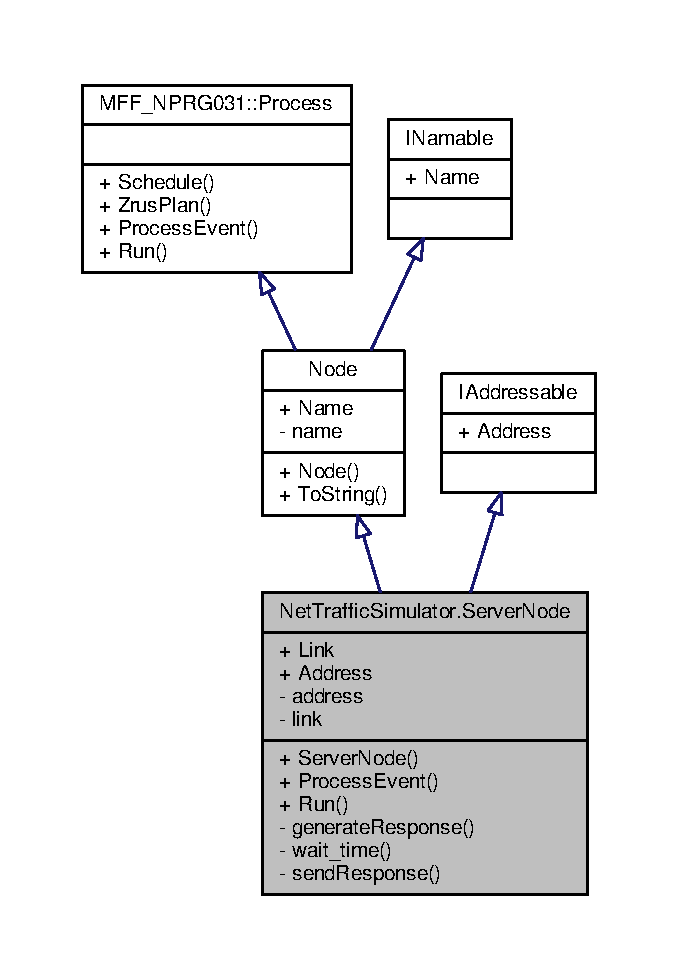
\includegraphics[width=350pt]{classNetTrafficSimulator_1_1ServerNode__inherit__graph}
\end{center}
\end{figure}


Collaboration diagram for Net\-Traffic\-Simulator.\-Server\-Node\-:
\nopagebreak
\begin{figure}[H]
\begin{center}
\leavevmode
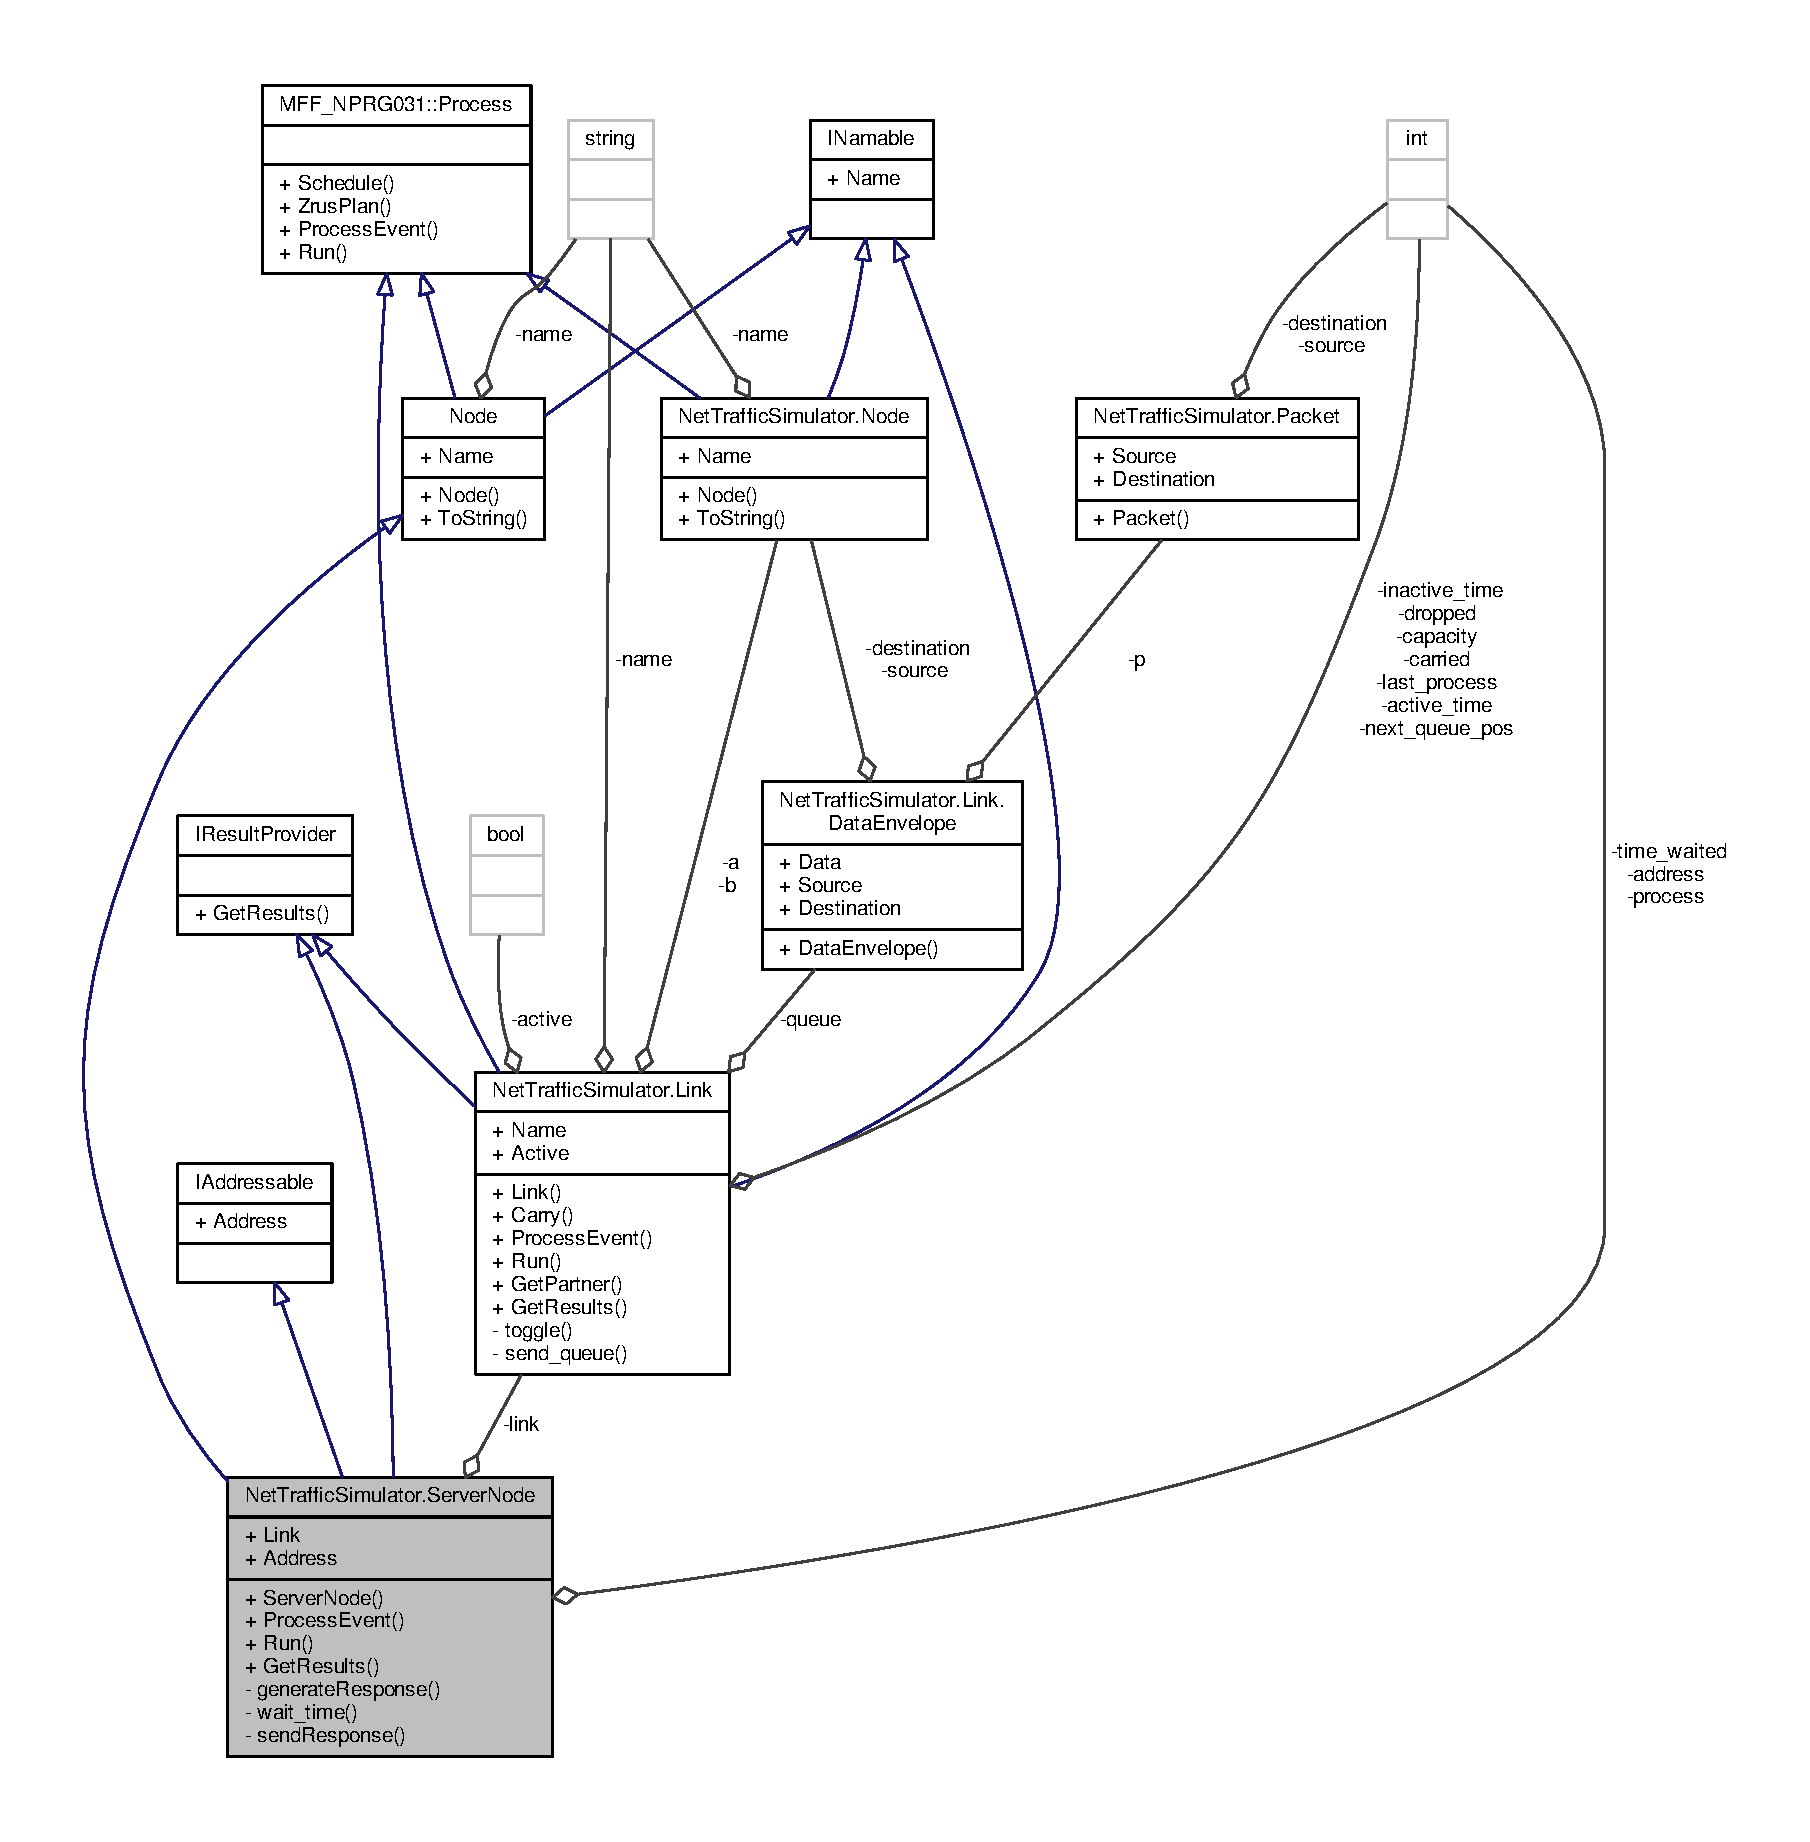
\includegraphics[width=350pt]{classNetTrafficSimulator_1_1ServerNode__coll__graph}
\end{center}
\end{figure}
\subsection*{Public Member Functions}
\begin{DoxyCompactItemize}
\item 
\hyperlink{classNetTrafficSimulator_1_1ServerNode_a0773c3d7230848f02282f217fcead9c3}{Server\-Node} (String \hyperlink{classNetTrafficSimulator_1_1Node_a679d5b6cca77c0cdb46cc98c347d4747}{name}, int \hyperlink{classNetTrafficSimulator_1_1ServerNode_a8be317d1e315710190755e4560fea3ef}{address})
\item 
override void \hyperlink{classNetTrafficSimulator_1_1ServerNode_ab309ebda509474d7a7f14b60955e5f98}{Process\-Event} (\hyperlink{classMFF__NPRG031_1_1State}{M\-F\-F\-\_\-\-N\-P\-R\-G031.\-State} state, \hyperlink{classMFF__NPRG031_1_1Model}{M\-F\-F\-\_\-\-N\-P\-R\-G031.\-Model} model)
\item 
override void \hyperlink{classNetTrafficSimulator_1_1ServerNode_aec78a48eea4006df1b4bce59ef17fbf7}{Run} (\hyperlink{classMFF__NPRG031_1_1Model}{M\-F\-F\-\_\-\-N\-P\-R\-G031.\-Model} m)
\item 
Dictionary$<$ string, object $>$ \hyperlink{classNetTrafficSimulator_1_1ServerNode_ab361087ec7201d5b8bdef1154d1315ef}{Get\-Results} (\hyperlink{classMFF__NPRG031_1_1Model}{M\-F\-F\-\_\-\-N\-P\-R\-G031.\-Model} model)
\end{DoxyCompactItemize}
\subsection*{Properties}
\begin{DoxyCompactItemize}
\item 
\hyperlink{classNetTrafficSimulator_1_1Link}{Link} \hyperlink{classNetTrafficSimulator_1_1ServerNode_a2fb3b251c8ad36760f68b8f7f4bc4c5b}{Link}\hspace{0.3cm}{\ttfamily  \mbox{[}get, set\mbox{]}}
\item 
int \hyperlink{classNetTrafficSimulator_1_1ServerNode_a52165503cd66de69748e5e4e5b9cedd4}{Address}\hspace{0.3cm}{\ttfamily  \mbox{[}get\mbox{]}}
\end{DoxyCompactItemize}
\subsection*{Private Member Functions}
\begin{DoxyCompactItemize}
\item 
\hyperlink{classNetTrafficSimulator_1_1Packet}{Packet} \hyperlink{classNetTrafficSimulator_1_1ServerNode_a96f3601328b5a86e3d69dcf93abafb34}{generate\-Response} (\hyperlink{classNetTrafficSimulator_1_1Packet}{Packet} p)
\item 
int \hyperlink{classNetTrafficSimulator_1_1ServerNode_a95a09cca40cf33abb200fa8c704f00a3}{wait\-\_\-time} ()
\item 
void \hyperlink{classNetTrafficSimulator_1_1ServerNode_ae90b2eb0a3abc8449a790a388dc1bcbb}{send\-Response} (\hyperlink{classNetTrafficSimulator_1_1Packet}{Packet} p, int time)
\end{DoxyCompactItemize}
\subsection*{Private Attributes}
\begin{DoxyCompactItemize}
\item 
readonly int \hyperlink{classNetTrafficSimulator_1_1ServerNode_a8be317d1e315710190755e4560fea3ef}{address}
\item 
int \hyperlink{classNetTrafficSimulator_1_1ServerNode_a3f25232ed46f3f83be0974fe060e390a}{time\-\_\-waited}
\item 
int \hyperlink{classNetTrafficSimulator_1_1ServerNode_a53521427dc9fa8eb16a461c4040d1b41}{process}
\item 
\hyperlink{classNetTrafficSimulator_1_1Link}{Link} \hyperlink{classNetTrafficSimulator_1_1ServerNode_a3968056516ee0dcb5ae111d09464efe6}{link}
\end{DoxyCompactItemize}


\subsection{Constructor \& Destructor Documentation}
\hypertarget{classNetTrafficSimulator_1_1ServerNode_a0773c3d7230848f02282f217fcead9c3}{\index{Net\-Traffic\-Simulator\-::\-Server\-Node@{Net\-Traffic\-Simulator\-::\-Server\-Node}!Server\-Node@{Server\-Node}}
\index{Server\-Node@{Server\-Node}!NetTrafficSimulator::ServerNode@{Net\-Traffic\-Simulator\-::\-Server\-Node}}
\subsubsection[{Server\-Node}]{\setlength{\rightskip}{0pt plus 5cm}Net\-Traffic\-Simulator.\-Server\-Node.\-Server\-Node (
\begin{DoxyParamCaption}
\item[{String}]{name, }
\item[{int}]{address}
\end{DoxyParamCaption}
)\hspace{0.3cm}{\ttfamily [inline]}}}\label{classNetTrafficSimulator_1_1ServerNode_a0773c3d7230848f02282f217fcead9c3}


\subsection{Member Function Documentation}
\hypertarget{classNetTrafficSimulator_1_1ServerNode_a96f3601328b5a86e3d69dcf93abafb34}{\index{Net\-Traffic\-Simulator\-::\-Server\-Node@{Net\-Traffic\-Simulator\-::\-Server\-Node}!generate\-Response@{generate\-Response}}
\index{generate\-Response@{generate\-Response}!NetTrafficSimulator::ServerNode@{Net\-Traffic\-Simulator\-::\-Server\-Node}}
\subsubsection[{generate\-Response}]{\setlength{\rightskip}{0pt plus 5cm}{\bf Packet} Net\-Traffic\-Simulator.\-Server\-Node.\-generate\-Response (
\begin{DoxyParamCaption}
\item[{{\bf Packet}}]{p}
\end{DoxyParamCaption}
)\hspace{0.3cm}{\ttfamily [inline]}, {\ttfamily [private]}}}\label{classNetTrafficSimulator_1_1ServerNode_a96f3601328b5a86e3d69dcf93abafb34}


Here is the caller graph for this function\-:\nopagebreak
\begin{figure}[H]
\begin{center}
\leavevmode
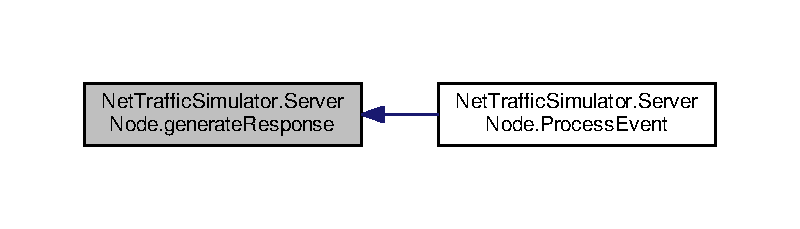
\includegraphics[width=350pt]{classNetTrafficSimulator_1_1ServerNode_a96f3601328b5a86e3d69dcf93abafb34_icgraph}
\end{center}
\end{figure}


\hypertarget{classNetTrafficSimulator_1_1ServerNode_ab361087ec7201d5b8bdef1154d1315ef}{\index{Net\-Traffic\-Simulator\-::\-Server\-Node@{Net\-Traffic\-Simulator\-::\-Server\-Node}!Get\-Results@{Get\-Results}}
\index{Get\-Results@{Get\-Results}!NetTrafficSimulator::ServerNode@{Net\-Traffic\-Simulator\-::\-Server\-Node}}
\subsubsection[{Get\-Results}]{\setlength{\rightskip}{0pt plus 5cm}Dictionary$<$string,object$>$ Net\-Traffic\-Simulator.\-Server\-Node.\-Get\-Results (
\begin{DoxyParamCaption}
\item[{{\bf M\-F\-F\-\_\-\-N\-P\-R\-G031.\-Model}}]{model}
\end{DoxyParamCaption}
)\hspace{0.3cm}{\ttfamily [inline]}}}\label{classNetTrafficSimulator_1_1ServerNode_ab361087ec7201d5b8bdef1154d1315ef}
Provide results measured during simulation for populating a result model \begin{DoxyReturn}{Returns}
Dictionary, where string is a key representing a human-\/readable description of measured data and object is value measured 
\end{DoxyReturn}


Implements \hyperlink{interfaceNetTrafficSimulator_1_1IResultProvider_ac7053c11f509ba1c2f653cd952b05323}{Net\-Traffic\-Simulator.\-I\-Result\-Provider}.

\hypertarget{classNetTrafficSimulator_1_1ServerNode_ab309ebda509474d7a7f14b60955e5f98}{\index{Net\-Traffic\-Simulator\-::\-Server\-Node@{Net\-Traffic\-Simulator\-::\-Server\-Node}!Process\-Event@{Process\-Event}}
\index{Process\-Event@{Process\-Event}!NetTrafficSimulator::ServerNode@{Net\-Traffic\-Simulator\-::\-Server\-Node}}
\subsubsection[{Process\-Event}]{\setlength{\rightskip}{0pt plus 5cm}override void Net\-Traffic\-Simulator.\-Server\-Node.\-Process\-Event (
\begin{DoxyParamCaption}
\item[{{\bf M\-F\-F\-\_\-\-N\-P\-R\-G031.\-State}}]{state, }
\item[{{\bf M\-F\-F\-\_\-\-N\-P\-R\-G031.\-Model}}]{model}
\end{DoxyParamCaption}
)\hspace{0.3cm}{\ttfamily [inline]}, {\ttfamily [virtual]}}}\label{classNetTrafficSimulator_1_1ServerNode_ab309ebda509474d7a7f14b60955e5f98}
Abstract method Process\-Event for process to react on event hapened 
\begin{DoxyParams}{Parameters}
{\em state} & In what state the process is now \\
\hline
{\em model} & Our simulation model \\
\hline
\end{DoxyParams}


Implements \hyperlink{classMFF__NPRG031_1_1Process_acb58d206e76c177264614d88f1818fdc}{M\-F\-F\-\_\-\-N\-P\-R\-G031.\-Process}.



Here is the call graph for this function\-:
\nopagebreak
\begin{figure}[H]
\begin{center}
\leavevmode
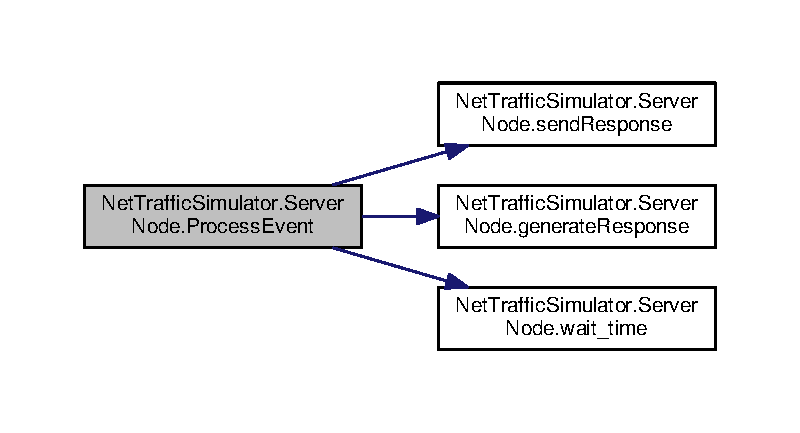
\includegraphics[width=350pt]{classNetTrafficSimulator_1_1ServerNode_ab309ebda509474d7a7f14b60955e5f98_cgraph}
\end{center}
\end{figure}


\hypertarget{classNetTrafficSimulator_1_1ServerNode_aec78a48eea4006df1b4bce59ef17fbf7}{\index{Net\-Traffic\-Simulator\-::\-Server\-Node@{Net\-Traffic\-Simulator\-::\-Server\-Node}!Run@{Run}}
\index{Run@{Run}!NetTrafficSimulator::ServerNode@{Net\-Traffic\-Simulator\-::\-Server\-Node}}
\subsubsection[{Run}]{\setlength{\rightskip}{0pt plus 5cm}override void Net\-Traffic\-Simulator.\-Server\-Node.\-Run (
\begin{DoxyParamCaption}
\item[{{\bf M\-F\-F\-\_\-\-N\-P\-R\-G031.\-Model}}]{m}
\end{DoxyParamCaption}
)\hspace{0.3cm}{\ttfamily [inline]}, {\ttfamily [virtual]}}}\label{classNetTrafficSimulator_1_1ServerNode_aec78a48eea4006df1b4bce59ef17fbf7}
Initial set up 
\begin{DoxyParams}{Parameters}
{\em m} & Model given \\
\hline
\end{DoxyParams}


Implements \hyperlink{classMFF__NPRG031_1_1Process_ad0e440dee98ba26c59ab22a60ebcafdd}{M\-F\-F\-\_\-\-N\-P\-R\-G031.\-Process}.

\hypertarget{classNetTrafficSimulator_1_1ServerNode_ae90b2eb0a3abc8449a790a388dc1bcbb}{\index{Net\-Traffic\-Simulator\-::\-Server\-Node@{Net\-Traffic\-Simulator\-::\-Server\-Node}!send\-Response@{send\-Response}}
\index{send\-Response@{send\-Response}!NetTrafficSimulator::ServerNode@{Net\-Traffic\-Simulator\-::\-Server\-Node}}
\subsubsection[{send\-Response}]{\setlength{\rightskip}{0pt plus 5cm}void Net\-Traffic\-Simulator.\-Server\-Node.\-send\-Response (
\begin{DoxyParamCaption}
\item[{{\bf Packet}}]{p, }
\item[{int}]{time}
\end{DoxyParamCaption}
)\hspace{0.3cm}{\ttfamily [inline]}, {\ttfamily [private]}}}\label{classNetTrafficSimulator_1_1ServerNode_ae90b2eb0a3abc8449a790a388dc1bcbb}


Here is the caller graph for this function\-:\nopagebreak
\begin{figure}[H]
\begin{center}
\leavevmode
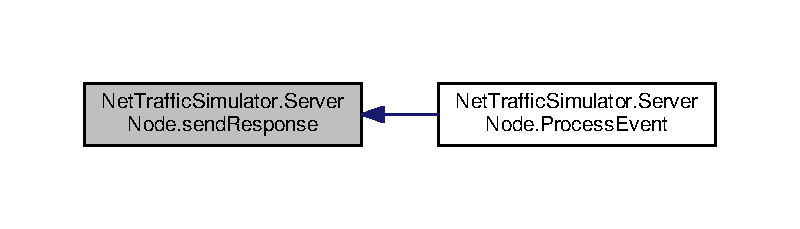
\includegraphics[width=350pt]{classNetTrafficSimulator_1_1ServerNode_ae90b2eb0a3abc8449a790a388dc1bcbb_icgraph}
\end{center}
\end{figure}


\hypertarget{classNetTrafficSimulator_1_1ServerNode_a95a09cca40cf33abb200fa8c704f00a3}{\index{Net\-Traffic\-Simulator\-::\-Server\-Node@{Net\-Traffic\-Simulator\-::\-Server\-Node}!wait\-\_\-time@{wait\-\_\-time}}
\index{wait\-\_\-time@{wait\-\_\-time}!NetTrafficSimulator::ServerNode@{Net\-Traffic\-Simulator\-::\-Server\-Node}}
\subsubsection[{wait\-\_\-time}]{\setlength{\rightskip}{0pt plus 5cm}int Net\-Traffic\-Simulator.\-Server\-Node.\-wait\-\_\-time (
\begin{DoxyParamCaption}
{}
\end{DoxyParamCaption}
)\hspace{0.3cm}{\ttfamily [inline]}, {\ttfamily [private]}}}\label{classNetTrafficSimulator_1_1ServerNode_a95a09cca40cf33abb200fa8c704f00a3}


Here is the caller graph for this function\-:\nopagebreak
\begin{figure}[H]
\begin{center}
\leavevmode
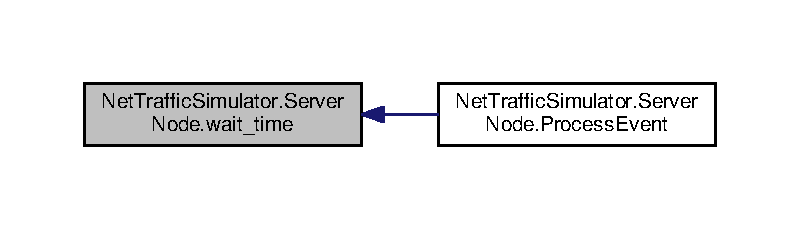
\includegraphics[width=350pt]{classNetTrafficSimulator_1_1ServerNode_a95a09cca40cf33abb200fa8c704f00a3_icgraph}
\end{center}
\end{figure}




\subsection{Member Data Documentation}
\hypertarget{classNetTrafficSimulator_1_1ServerNode_a8be317d1e315710190755e4560fea3ef}{\index{Net\-Traffic\-Simulator\-::\-Server\-Node@{Net\-Traffic\-Simulator\-::\-Server\-Node}!address@{address}}
\index{address@{address}!NetTrafficSimulator::ServerNode@{Net\-Traffic\-Simulator\-::\-Server\-Node}}
\subsubsection[{address}]{\setlength{\rightskip}{0pt plus 5cm}readonly int Net\-Traffic\-Simulator.\-Server\-Node.\-address\hspace{0.3cm}{\ttfamily [private]}}}\label{classNetTrafficSimulator_1_1ServerNode_a8be317d1e315710190755e4560fea3ef}
\hypertarget{classNetTrafficSimulator_1_1ServerNode_a3968056516ee0dcb5ae111d09464efe6}{\index{Net\-Traffic\-Simulator\-::\-Server\-Node@{Net\-Traffic\-Simulator\-::\-Server\-Node}!link@{link}}
\index{link@{link}!NetTrafficSimulator::ServerNode@{Net\-Traffic\-Simulator\-::\-Server\-Node}}
\subsubsection[{link}]{\setlength{\rightskip}{0pt plus 5cm}{\bf Link} Net\-Traffic\-Simulator.\-Server\-Node.\-link\hspace{0.3cm}{\ttfamily [private]}}}\label{classNetTrafficSimulator_1_1ServerNode_a3968056516ee0dcb5ae111d09464efe6}
\hypertarget{classNetTrafficSimulator_1_1ServerNode_a53521427dc9fa8eb16a461c4040d1b41}{\index{Net\-Traffic\-Simulator\-::\-Server\-Node@{Net\-Traffic\-Simulator\-::\-Server\-Node}!process@{process}}
\index{process@{process}!NetTrafficSimulator::ServerNode@{Net\-Traffic\-Simulator\-::\-Server\-Node}}
\subsubsection[{process}]{\setlength{\rightskip}{0pt plus 5cm}int Net\-Traffic\-Simulator.\-Server\-Node.\-process\hspace{0.3cm}{\ttfamily [private]}}}\label{classNetTrafficSimulator_1_1ServerNode_a53521427dc9fa8eb16a461c4040d1b41}
\hypertarget{classNetTrafficSimulator_1_1ServerNode_a3f25232ed46f3f83be0974fe060e390a}{\index{Net\-Traffic\-Simulator\-::\-Server\-Node@{Net\-Traffic\-Simulator\-::\-Server\-Node}!time\-\_\-waited@{time\-\_\-waited}}
\index{time\-\_\-waited@{time\-\_\-waited}!NetTrafficSimulator::ServerNode@{Net\-Traffic\-Simulator\-::\-Server\-Node}}
\subsubsection[{time\-\_\-waited}]{\setlength{\rightskip}{0pt plus 5cm}int Net\-Traffic\-Simulator.\-Server\-Node.\-time\-\_\-waited\hspace{0.3cm}{\ttfamily [private]}}}\label{classNetTrafficSimulator_1_1ServerNode_a3f25232ed46f3f83be0974fe060e390a}


\subsection{Property Documentation}
\hypertarget{classNetTrafficSimulator_1_1ServerNode_a52165503cd66de69748e5e4e5b9cedd4}{\index{Net\-Traffic\-Simulator\-::\-Server\-Node@{Net\-Traffic\-Simulator\-::\-Server\-Node}!Address@{Address}}
\index{Address@{Address}!NetTrafficSimulator::ServerNode@{Net\-Traffic\-Simulator\-::\-Server\-Node}}
\subsubsection[{Address}]{\setlength{\rightskip}{0pt plus 5cm}int Net\-Traffic\-Simulator.\-Server\-Node.\-Address\hspace{0.3cm}{\ttfamily [get]}}}\label{classNetTrafficSimulator_1_1ServerNode_a52165503cd66de69748e5e4e5b9cedd4}
\hypertarget{classNetTrafficSimulator_1_1ServerNode_a2fb3b251c8ad36760f68b8f7f4bc4c5b}{\index{Net\-Traffic\-Simulator\-::\-Server\-Node@{Net\-Traffic\-Simulator\-::\-Server\-Node}!Link@{Link}}
\index{Link@{Link}!NetTrafficSimulator::ServerNode@{Net\-Traffic\-Simulator\-::\-Server\-Node}}
\subsubsection[{Link}]{\setlength{\rightskip}{0pt plus 5cm}{\bf Link} Net\-Traffic\-Simulator.\-Server\-Node.\-Link\hspace{0.3cm}{\ttfamily [get]}, {\ttfamily [set]}}}\label{classNetTrafficSimulator_1_1ServerNode_a2fb3b251c8ad36760f68b8f7f4bc4c5b}


The documentation for this class was generated from the following file\-:\begin{DoxyCompactItemize}
\item 
Net\-Traffic\-Simulator/\-Net\-Traffic\-Simulator/framework/extension/\hyperlink{ServerNode_8cs}{Server\-Node.\-cs}\end{DoxyCompactItemize}

\hypertarget{classNetTrafficSimulator_1_1SimulationController}{\section{Net\-Traffic\-Simulator.\-Simulation\-Controller Class Reference}
\label{classNetTrafficSimulator_1_1SimulationController}\index{Net\-Traffic\-Simulator.\-Simulation\-Controller@{Net\-Traffic\-Simulator.\-Simulation\-Controller}}
}


Collaboration diagram for Net\-Traffic\-Simulator.\-Simulation\-Controller\-:\nopagebreak
\begin{figure}[H]
\begin{center}
\leavevmode
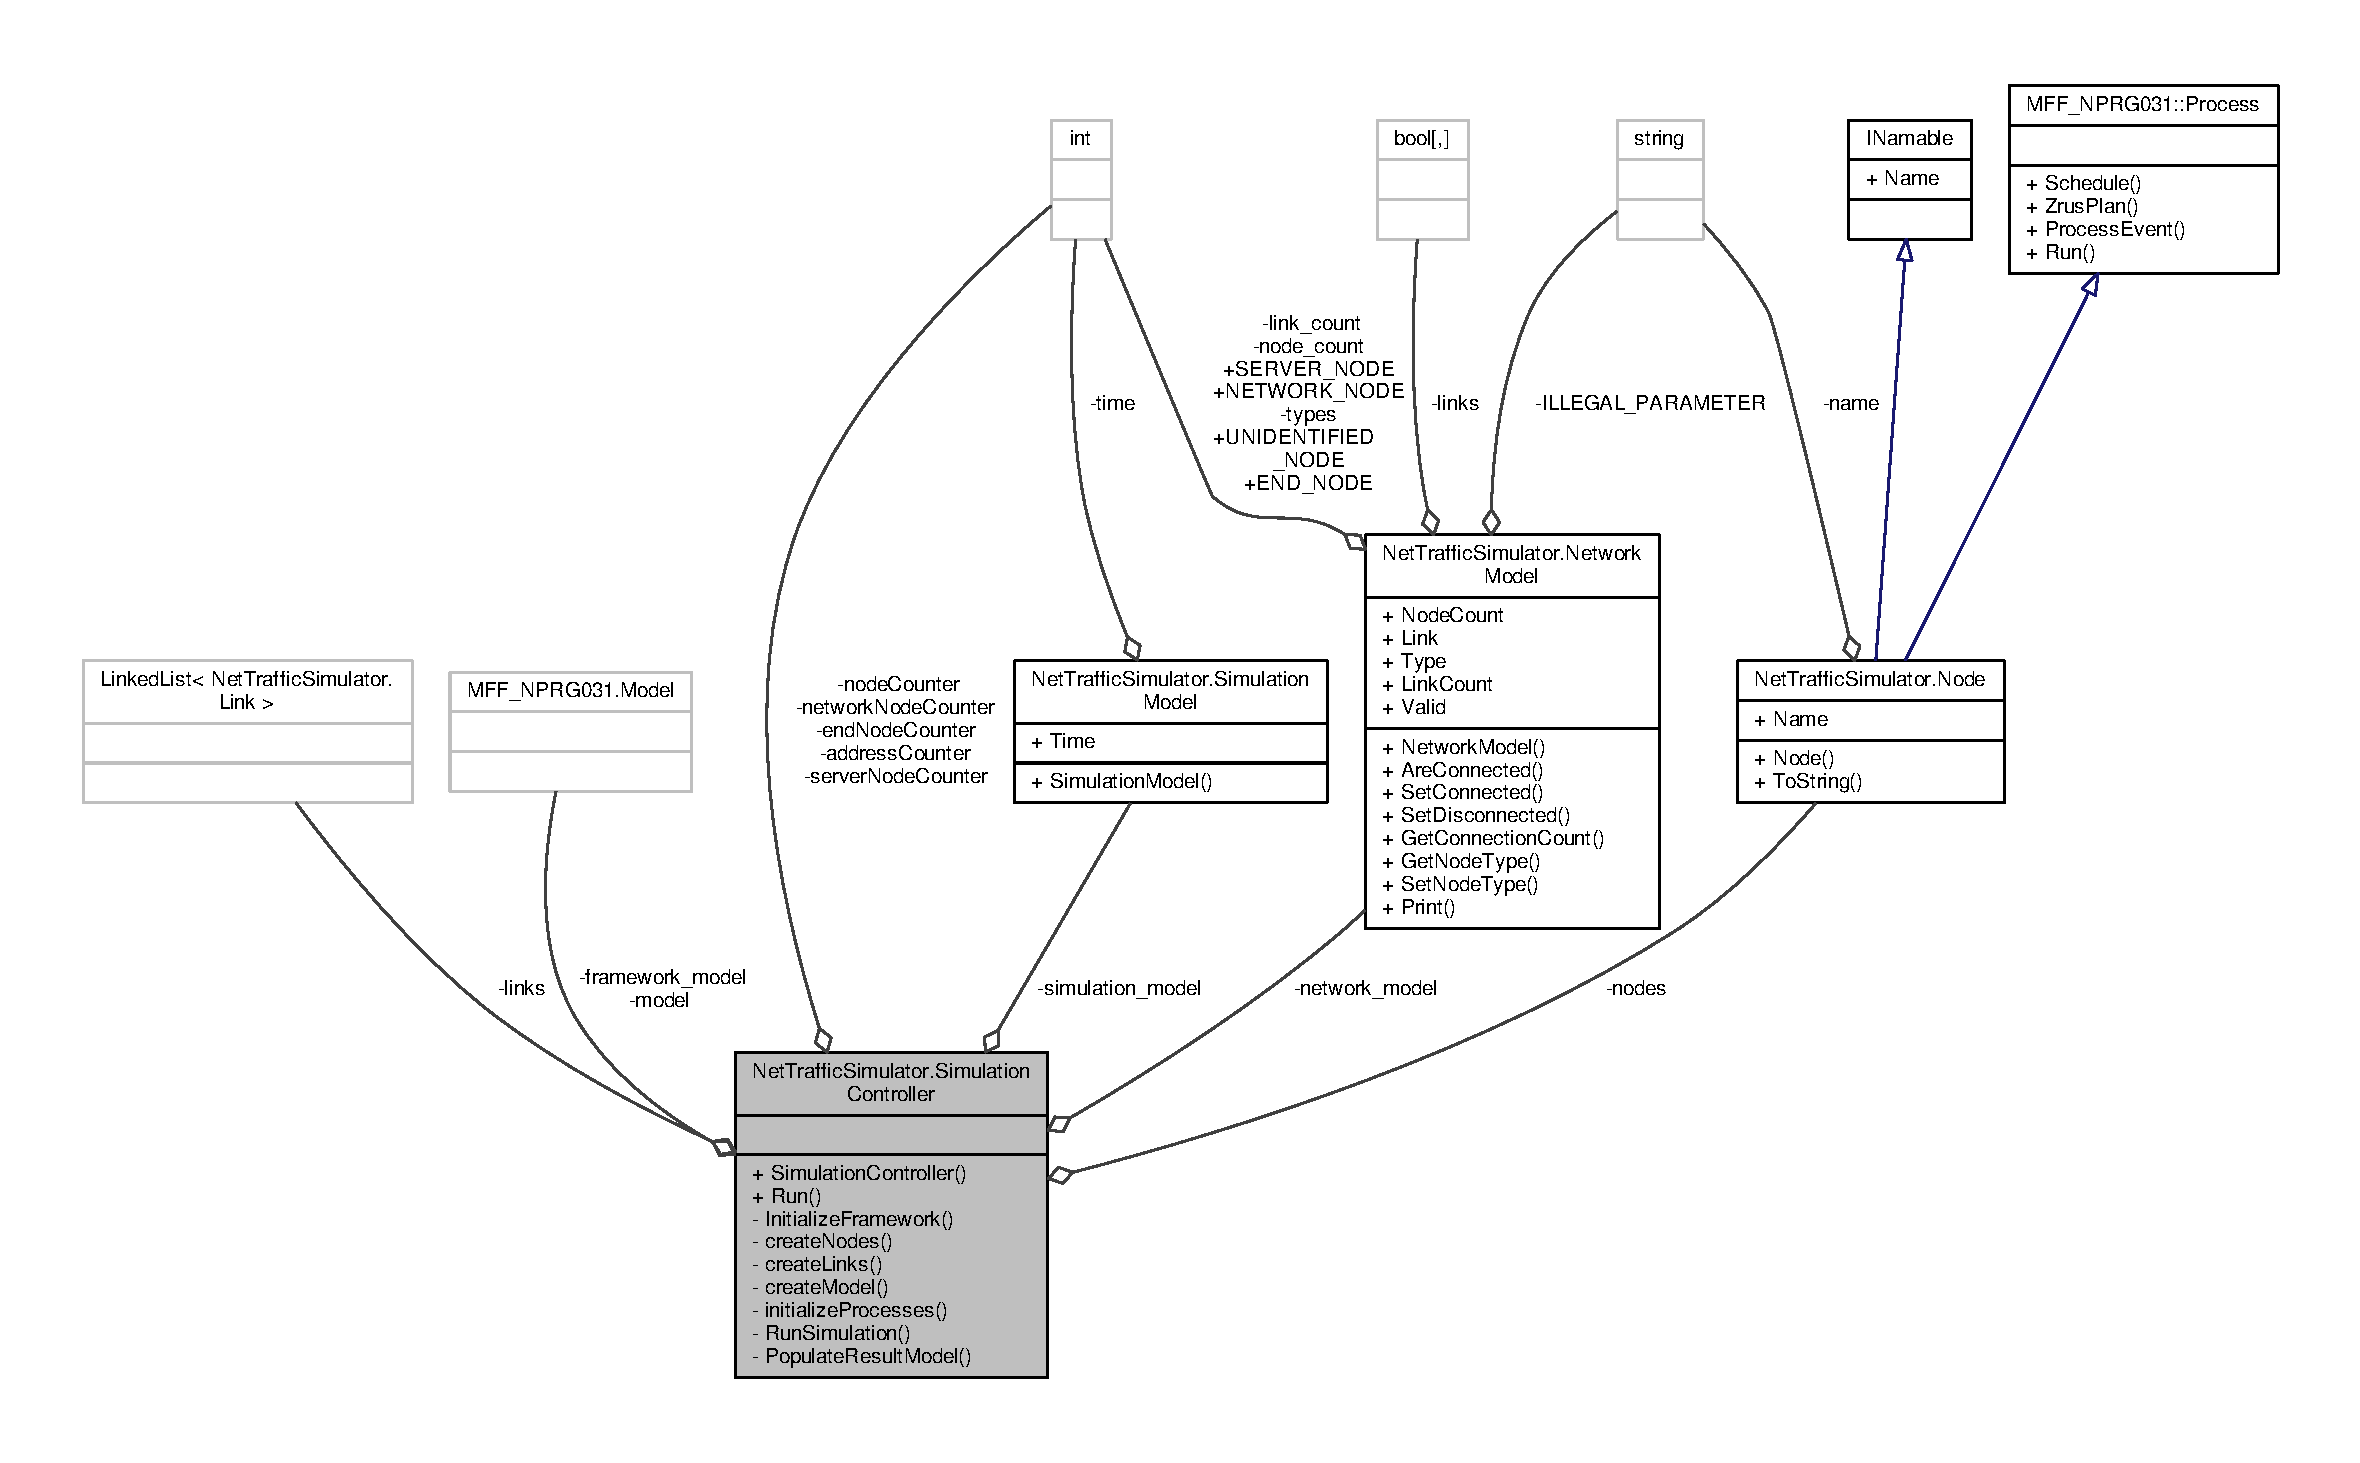
\includegraphics[width=350pt]{classNetTrafficSimulator_1_1SimulationController__coll__graph}
\end{center}
\end{figure}
\subsection*{Public Member Functions}
\begin{DoxyCompactItemize}
\item 
\hyperlink{classNetTrafficSimulator_1_1SimulationController_a30890df3e3b1ce4cef47fe597afa58f2}{Simulation\-Controller} (\hyperlink{classNetTrafficSimulator_1_1NetworkModel}{Network\-Model} nm, \hyperlink{classNetTrafficSimulator_1_1SimulationModel}{Simulation\-Model} sm)
\item 
void \hyperlink{classNetTrafficSimulator_1_1SimulationController_a22dedb5c0d0233bfa7acfc858af4a0cf}{Run} ()
\end{DoxyCompactItemize}
\subsection*{Private Member Functions}
\begin{DoxyCompactItemize}
\item 
void \hyperlink{classNetTrafficSimulator_1_1SimulationController_aee0204844a793fc1e26e1940f8c3f1e3}{Initialize\-Framework} ()
\item 
void \hyperlink{classNetTrafficSimulator_1_1SimulationController_aaa2dfff1b6c614ec8202cac5f0aea58c}{create\-Nodes} ()
\item 
void \hyperlink{classNetTrafficSimulator_1_1SimulationController_a65bdc4b66235a69672fda176b1937bc7}{create\-Links} ()
\item 
void \hyperlink{classNetTrafficSimulator_1_1SimulationController_ad23685dbec3fce89fc4fa615edef1150}{create\-Model} ()
\item 
void \hyperlink{classNetTrafficSimulator_1_1SimulationController_a893854760ab4e24a432ab72aa1f20d1a}{initialize\-Processes} ()
\item 
void \hyperlink{classNetTrafficSimulator_1_1SimulationController_ac72e9edb9b5ab11d579be22ee0029294}{Run\-Simulation} ()
\item 
void \hyperlink{classNetTrafficSimulator_1_1SimulationController_ae40f65ccc6e418355c89294d3dddca5a}{Populate\-Result\-Model} ()
\end{DoxyCompactItemize}
\subsection*{Private Attributes}
\begin{DoxyCompactItemize}
\item 
\hyperlink{classNetTrafficSimulator_1_1NetworkModel}{Network\-Model} \hyperlink{classNetTrafficSimulator_1_1SimulationController_a80c4b1d3b982e591f530bf5877b259fa}{network\-\_\-model}
\item 
\hyperlink{classNetTrafficSimulator_1_1SimulationModel}{Simulation\-Model} \hyperlink{classNetTrafficSimulator_1_1SimulationController_a26441a135203881caae479f93f17e288}{simulation\-\_\-model}
\item 
\hyperlink{classMFF__NPRG031_1_1Model}{M\-F\-F\-\_\-\-N\-P\-R\-G031.\-Model} \hyperlink{classNetTrafficSimulator_1_1SimulationController_a3037a65e37c5c5e894bc584b8fe5c12d}{framework\-\_\-model}
\item 
int \hyperlink{classNetTrafficSimulator_1_1SimulationController_a9d07f9372ee5eeacefcb4d0448122f6d}{end\-Node\-Counter}
\item 
int \hyperlink{classNetTrafficSimulator_1_1SimulationController_a2b2363037a31bae97e4aede4af2512c4}{network\-Node\-Counter}
\item 
int \hyperlink{classNetTrafficSimulator_1_1SimulationController_a59a626f2fc2b81873ef548f2d7d04948}{server\-Node\-Counter}
\item 
int \hyperlink{classNetTrafficSimulator_1_1SimulationController_a79f2fd9be4b8d9070494975f9d470563}{address\-Counter}
\item 
int \hyperlink{classNetTrafficSimulator_1_1SimulationController_ada67d39ff4d7f0595b295b895216abf4}{node\-Counter}
\item 
\hyperlink{classNetTrafficSimulator_1_1Node}{Node}\mbox{[}$\,$\mbox{]} \hyperlink{classNetTrafficSimulator_1_1SimulationController_a63041df0cb83bab3ee4db1505656e806}{nodes}
\item 
Linked\-List$<$ \hyperlink{classNetTrafficSimulator_1_1Link}{Link} $>$ \hyperlink{classNetTrafficSimulator_1_1SimulationController_a5c83a56d28d5336e08efd3d893e47381}{links}
\item 
\hyperlink{classMFF__NPRG031_1_1Model}{M\-F\-F\-\_\-\-N\-P\-R\-G031.\-Model} \hyperlink{classNetTrafficSimulator_1_1SimulationController_a28227ccfab6fb0d8e41ae0975ee7a5af}{model}
\end{DoxyCompactItemize}


\subsection{Detailed Description}
Simulation controller takes data from \hyperlink{classNetTrafficSimulator_1_1NetworkModel}{Network\-Model} and \hyperlink{classNetTrafficSimulator_1_1SimulationModel}{Simulation\-Model} and sets up simulation framework 

\subsection{Constructor \& Destructor Documentation}
\hypertarget{classNetTrafficSimulator_1_1SimulationController_a30890df3e3b1ce4cef47fe597afa58f2}{\index{Net\-Traffic\-Simulator\-::\-Simulation\-Controller@{Net\-Traffic\-Simulator\-::\-Simulation\-Controller}!Simulation\-Controller@{Simulation\-Controller}}
\index{Simulation\-Controller@{Simulation\-Controller}!NetTrafficSimulator::SimulationController@{Net\-Traffic\-Simulator\-::\-Simulation\-Controller}}
\subsubsection[{Simulation\-Controller}]{\setlength{\rightskip}{0pt plus 5cm}Net\-Traffic\-Simulator.\-Simulation\-Controller.\-Simulation\-Controller (
\begin{DoxyParamCaption}
\item[{{\bf Network\-Model}}]{nm, }
\item[{{\bf Simulation\-Model}}]{sm}
\end{DoxyParamCaption}
)\hspace{0.3cm}{\ttfamily [inline]}}}\label{classNetTrafficSimulator_1_1SimulationController_a30890df3e3b1ce4cef47fe597afa58f2}
Constructor stores Network and Simulation models for future reference 
\begin{DoxyParams}{Parameters}
{\em nm} & Network Model \\
\hline
{\em sm} & Simulation Model \\
\hline
\end{DoxyParams}

\begin{DoxyExceptions}{Exceptions}
{\em Argument\-Exception} & If any of models is null or the network model provided is not valid \\
\hline
\end{DoxyExceptions}


\subsection{Member Function Documentation}
\hypertarget{classNetTrafficSimulator_1_1SimulationController_a65bdc4b66235a69672fda176b1937bc7}{\index{Net\-Traffic\-Simulator\-::\-Simulation\-Controller@{Net\-Traffic\-Simulator\-::\-Simulation\-Controller}!create\-Links@{create\-Links}}
\index{create\-Links@{create\-Links}!NetTrafficSimulator::SimulationController@{Net\-Traffic\-Simulator\-::\-Simulation\-Controller}}
\subsubsection[{create\-Links}]{\setlength{\rightskip}{0pt plus 5cm}void Net\-Traffic\-Simulator.\-Simulation\-Controller.\-create\-Links (
\begin{DoxyParamCaption}
{}
\end{DoxyParamCaption}
)\hspace{0.3cm}{\ttfamily [inline]}, {\ttfamily [private]}}}\label{classNetTrafficSimulator_1_1SimulationController_a65bdc4b66235a69672fda176b1937bc7}
For each pair of nodes where connection is marked, create a new \hyperlink{classNetTrafficSimulator_1_1Link}{Link} instance and register the link to each node. New links are stored in Linked\-List$<$\-Link$>$ links initialized here (as their count is unknown)

As link capacities are not supported by \hyperlink{classNetTrafficSimulator_1_1NetworkModel}{Network\-Model} yet, all are set for 0 at this point.

Test is necessary to verify links are created properly according to the model


\begin{DoxyExceptions}{Exceptions}
{\em Invalid\-Operation\-Exception} & if any node is of unidentified type, the network model is null, the nodes array is null or length of the nodes array don't match node count in the network model \\
\hline
\end{DoxyExceptions}


Here is the call graph for this function\-:\nopagebreak
\begin{figure}[H]
\begin{center}
\leavevmode
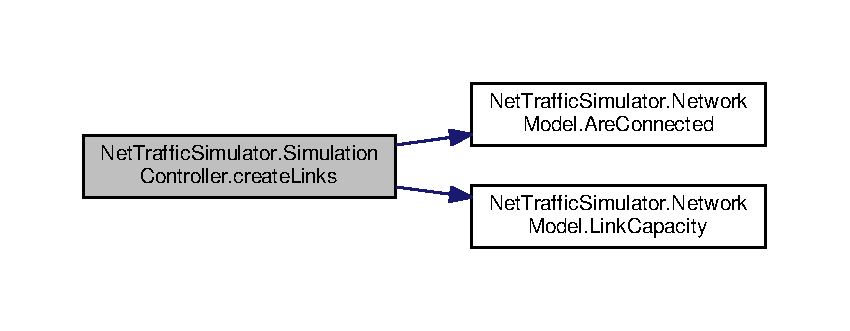
\includegraphics[width=350pt]{classNetTrafficSimulator_1_1SimulationController_a65bdc4b66235a69672fda176b1937bc7_cgraph}
\end{center}
\end{figure}




Here is the caller graph for this function\-:\nopagebreak
\begin{figure}[H]
\begin{center}
\leavevmode
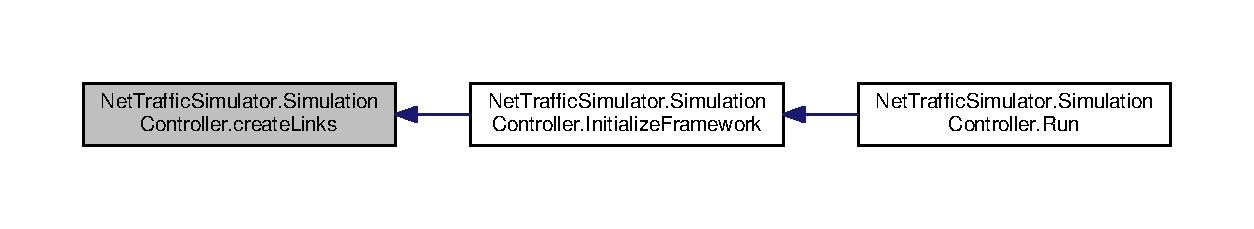
\includegraphics[width=350pt]{classNetTrafficSimulator_1_1SimulationController_a65bdc4b66235a69672fda176b1937bc7_icgraph}
\end{center}
\end{figure}


\hypertarget{classNetTrafficSimulator_1_1SimulationController_ad23685dbec3fce89fc4fa615edef1150}{\index{Net\-Traffic\-Simulator\-::\-Simulation\-Controller@{Net\-Traffic\-Simulator\-::\-Simulation\-Controller}!create\-Model@{create\-Model}}
\index{create\-Model@{create\-Model}!NetTrafficSimulator::SimulationController@{Net\-Traffic\-Simulator\-::\-Simulation\-Controller}}
\subsubsection[{create\-Model}]{\setlength{\rightskip}{0pt plus 5cm}void Net\-Traffic\-Simulator.\-Simulation\-Controller.\-create\-Model (
\begin{DoxyParamCaption}
{}
\end{DoxyParamCaption}
)\hspace{0.3cm}{\ttfamily [inline]}, {\ttfamily [private]}}}\label{classNetTrafficSimulator_1_1SimulationController_ad23685dbec3fce89fc4fa615edef1150}
Unless simulation model is null initialize Model with appropriate Time To Run 
\begin{DoxyExceptions}{Exceptions}
{\em Invalid\-Operation\-Exception} & if \hyperlink{classNetTrafficSimulator_1_1SimulationModel}{Simulation\-Model} is null \\
\hline
\end{DoxyExceptions}


Here is the caller graph for this function\-:\nopagebreak
\begin{figure}[H]
\begin{center}
\leavevmode
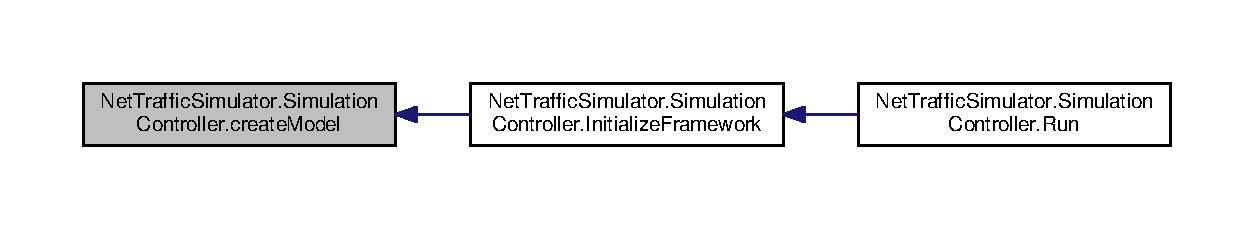
\includegraphics[width=350pt]{classNetTrafficSimulator_1_1SimulationController_ad23685dbec3fce89fc4fa615edef1150_icgraph}
\end{center}
\end{figure}


\hypertarget{classNetTrafficSimulator_1_1SimulationController_aaa2dfff1b6c614ec8202cac5f0aea58c}{\index{Net\-Traffic\-Simulator\-::\-Simulation\-Controller@{Net\-Traffic\-Simulator\-::\-Simulation\-Controller}!create\-Nodes@{create\-Nodes}}
\index{create\-Nodes@{create\-Nodes}!NetTrafficSimulator::SimulationController@{Net\-Traffic\-Simulator\-::\-Simulation\-Controller}}
\subsubsection[{create\-Nodes}]{\setlength{\rightskip}{0pt plus 5cm}void Net\-Traffic\-Simulator.\-Simulation\-Controller.\-create\-Nodes (
\begin{DoxyParamCaption}
{}
\end{DoxyParamCaption}
)\hspace{0.3cm}{\ttfamily [inline]}, {\ttfamily [private]}}}\label{classNetTrafficSimulator_1_1SimulationController_aaa2dfff1b6c614ec8202cac5f0aea58c}
For each node in Network Model create an appropriate \hyperlink{classNetTrafficSimulator_1_1Node}{Node} instance and store it in nodes array. Nodes array and counters are initialized here. Address generated here for nodes requiring an address. 
\begin{DoxyExceptions}{Exceptions}
{\em Invalid\-Operation\-Exception} & if found unidentified node type \\
\hline
\end{DoxyExceptions}


Here is the call graph for this function\-:\nopagebreak
\begin{figure}[H]
\begin{center}
\leavevmode
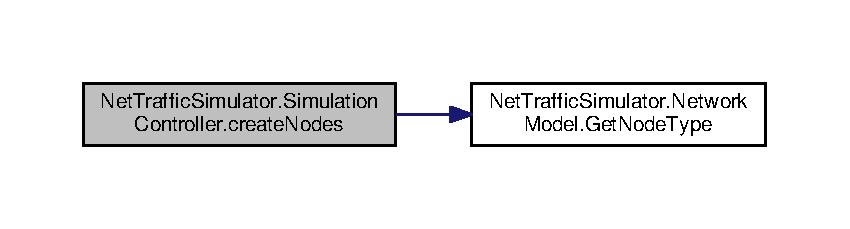
\includegraphics[width=350pt]{classNetTrafficSimulator_1_1SimulationController_aaa2dfff1b6c614ec8202cac5f0aea58c_cgraph}
\end{center}
\end{figure}




Here is the caller graph for this function\-:\nopagebreak
\begin{figure}[H]
\begin{center}
\leavevmode
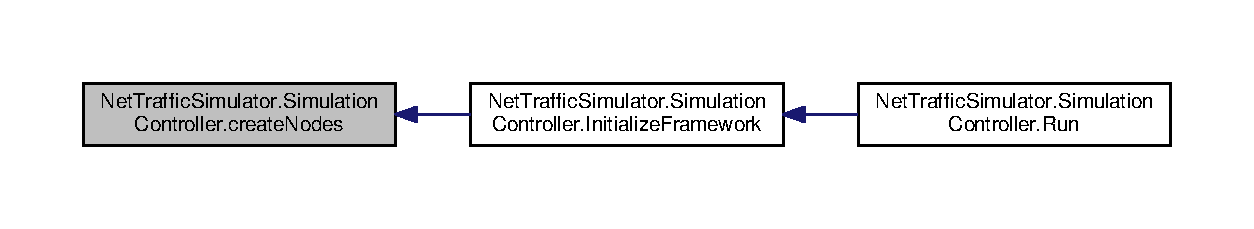
\includegraphics[width=350pt]{classNetTrafficSimulator_1_1SimulationController_aaa2dfff1b6c614ec8202cac5f0aea58c_icgraph}
\end{center}
\end{figure}


\hypertarget{classNetTrafficSimulator_1_1SimulationController_aee0204844a793fc1e26e1940f8c3f1e3}{\index{Net\-Traffic\-Simulator\-::\-Simulation\-Controller@{Net\-Traffic\-Simulator\-::\-Simulation\-Controller}!Initialize\-Framework@{Initialize\-Framework}}
\index{Initialize\-Framework@{Initialize\-Framework}!NetTrafficSimulator::SimulationController@{Net\-Traffic\-Simulator\-::\-Simulation\-Controller}}
\subsubsection[{Initialize\-Framework}]{\setlength{\rightskip}{0pt plus 5cm}void Net\-Traffic\-Simulator.\-Simulation\-Controller.\-Initialize\-Framework (
\begin{DoxyParamCaption}
{}
\end{DoxyParamCaption}
)\hspace{0.3cm}{\ttfamily [inline]}, {\ttfamily [private]}}}\label{classNetTrafficSimulator_1_1SimulationController_aee0204844a793fc1e26e1940f8c3f1e3}
Initializes simulation framework\-: create Model, create necessary Nodes, set them up and place into Calendar 

Here is the call graph for this function\-:\nopagebreak
\begin{figure}[H]
\begin{center}
\leavevmode
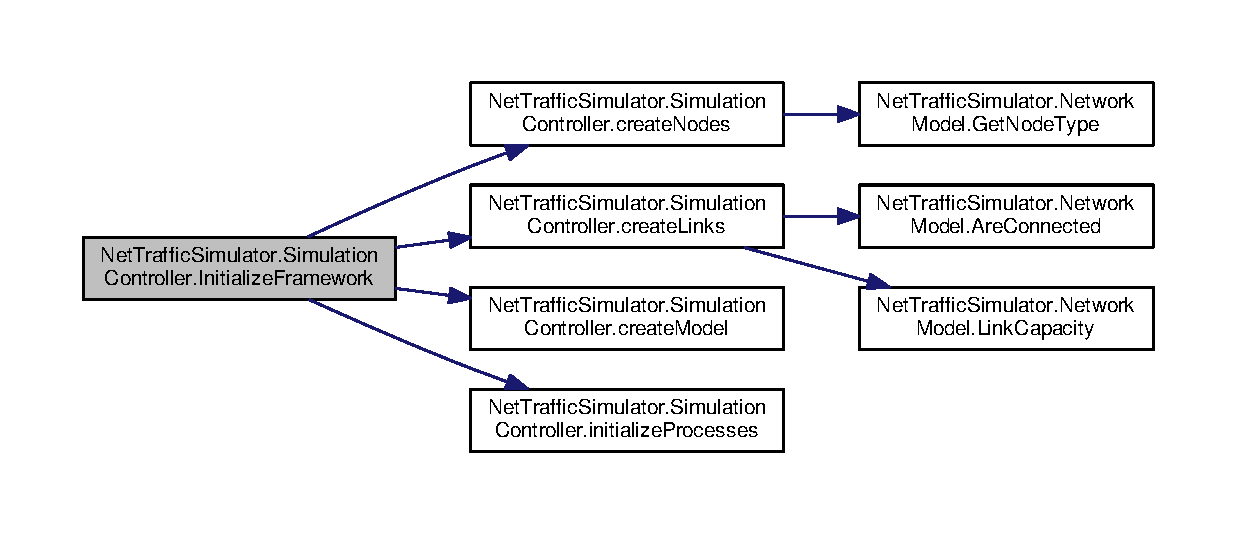
\includegraphics[width=350pt]{classNetTrafficSimulator_1_1SimulationController_aee0204844a793fc1e26e1940f8c3f1e3_cgraph}
\end{center}
\end{figure}




Here is the caller graph for this function\-:\nopagebreak
\begin{figure}[H]
\begin{center}
\leavevmode
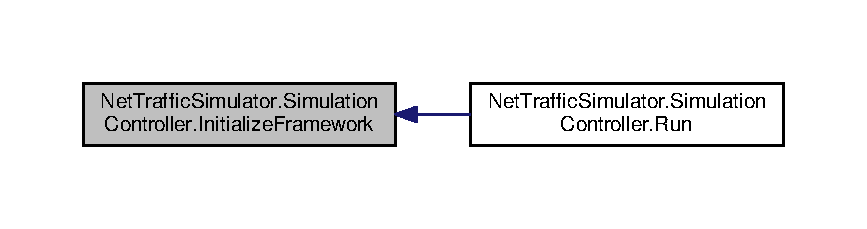
\includegraphics[width=350pt]{classNetTrafficSimulator_1_1SimulationController_aee0204844a793fc1e26e1940f8c3f1e3_icgraph}
\end{center}
\end{figure}


\hypertarget{classNetTrafficSimulator_1_1SimulationController_a893854760ab4e24a432ab72aa1f20d1a}{\index{Net\-Traffic\-Simulator\-::\-Simulation\-Controller@{Net\-Traffic\-Simulator\-::\-Simulation\-Controller}!initialize\-Processes@{initialize\-Processes}}
\index{initialize\-Processes@{initialize\-Processes}!NetTrafficSimulator::SimulationController@{Net\-Traffic\-Simulator\-::\-Simulation\-Controller}}
\subsubsection[{initialize\-Processes}]{\setlength{\rightskip}{0pt plus 5cm}void Net\-Traffic\-Simulator.\-Simulation\-Controller.\-initialize\-Processes (
\begin{DoxyParamCaption}
{}
\end{DoxyParamCaption}
)\hspace{0.3cm}{\ttfamily [inline]}, {\ttfamily [private]}}}\label{classNetTrafficSimulator_1_1SimulationController_a893854760ab4e24a432ab72aa1f20d1a}
If Model is not null, invoke Run method on each \hyperlink{classNetTrafficSimulator_1_1Node}{Node} and \hyperlink{classNetTrafficSimulator_1_1Link}{Link} registered 
\begin{DoxyExceptions}{Exceptions}
{\em Invalid\-Operation\-Exception} & if model is null (not created yet) \\
\hline
\end{DoxyExceptions}


Here is the caller graph for this function\-:\nopagebreak
\begin{figure}[H]
\begin{center}
\leavevmode
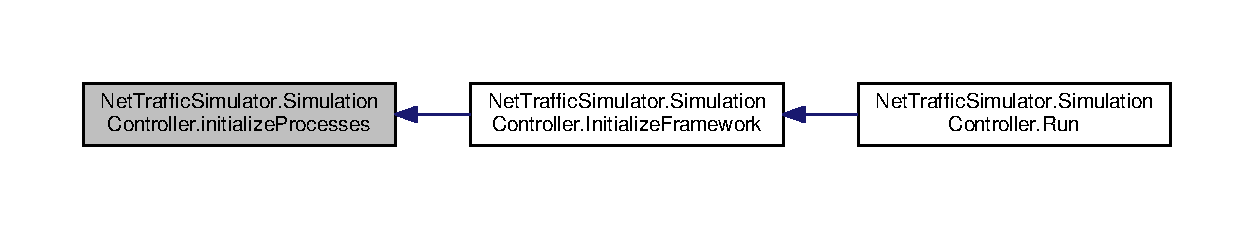
\includegraphics[width=350pt]{classNetTrafficSimulator_1_1SimulationController_a893854760ab4e24a432ab72aa1f20d1a_icgraph}
\end{center}
\end{figure}


\hypertarget{classNetTrafficSimulator_1_1SimulationController_ae40f65ccc6e418355c89294d3dddca5a}{\index{Net\-Traffic\-Simulator\-::\-Simulation\-Controller@{Net\-Traffic\-Simulator\-::\-Simulation\-Controller}!Populate\-Result\-Model@{Populate\-Result\-Model}}
\index{Populate\-Result\-Model@{Populate\-Result\-Model}!NetTrafficSimulator::SimulationController@{Net\-Traffic\-Simulator\-::\-Simulation\-Controller}}
\subsubsection[{Populate\-Result\-Model}]{\setlength{\rightskip}{0pt plus 5cm}void Net\-Traffic\-Simulator.\-Simulation\-Controller.\-Populate\-Result\-Model (
\begin{DoxyParamCaption}
{}
\end{DoxyParamCaption}
)\hspace{0.3cm}{\ttfamily [inline]}, {\ttfamily [private]}}}\label{classNetTrafficSimulator_1_1SimulationController_ae40f65ccc6e418355c89294d3dddca5a}
Stores statistics into Result Model unless this is done by Run\-Simulation 

Here is the caller graph for this function\-:\nopagebreak
\begin{figure}[H]
\begin{center}
\leavevmode
\includegraphics[width=350pt]{classNetTrafficSimulator_1_1SimulationController_ae40f65ccc6e418355c89294d3dddca5a_icgraph}
\end{center}
\end{figure}


\hypertarget{classNetTrafficSimulator_1_1SimulationController_a22dedb5c0d0233bfa7acfc858af4a0cf}{\index{Net\-Traffic\-Simulator\-::\-Simulation\-Controller@{Net\-Traffic\-Simulator\-::\-Simulation\-Controller}!Run@{Run}}
\index{Run@{Run}!NetTrafficSimulator::SimulationController@{Net\-Traffic\-Simulator\-::\-Simulation\-Controller}}
\subsubsection[{Run}]{\setlength{\rightskip}{0pt plus 5cm}void Net\-Traffic\-Simulator.\-Simulation\-Controller.\-Run (
\begin{DoxyParamCaption}
{}
\end{DoxyParamCaption}
)\hspace{0.3cm}{\ttfamily [inline]}}}\label{classNetTrafficSimulator_1_1SimulationController_a22dedb5c0d0233bfa7acfc858af4a0cf}
Initialize framework, run simulation, populate result model 

Here is the call graph for this function\-:\nopagebreak
\begin{figure}[H]
\begin{center}
\leavevmode
\includegraphics[width=350pt]{classNetTrafficSimulator_1_1SimulationController_a22dedb5c0d0233bfa7acfc858af4a0cf_cgraph}
\end{center}
\end{figure}


\hypertarget{classNetTrafficSimulator_1_1SimulationController_ac72e9edb9b5ab11d579be22ee0029294}{\index{Net\-Traffic\-Simulator\-::\-Simulation\-Controller@{Net\-Traffic\-Simulator\-::\-Simulation\-Controller}!Run\-Simulation@{Run\-Simulation}}
\index{Run\-Simulation@{Run\-Simulation}!NetTrafficSimulator::SimulationController@{Net\-Traffic\-Simulator\-::\-Simulation\-Controller}}
\subsubsection[{Run\-Simulation}]{\setlength{\rightskip}{0pt plus 5cm}void Net\-Traffic\-Simulator.\-Simulation\-Controller.\-Run\-Simulation (
\begin{DoxyParamCaption}
{}
\end{DoxyParamCaption}
)\hspace{0.3cm}{\ttfamily [inline]}, {\ttfamily [private]}}}\label{classNetTrafficSimulator_1_1SimulationController_ac72e9edb9b5ab11d579be22ee0029294}
Runs a simulation, stores statistics 

Here is the caller graph for this function\-:\nopagebreak
\begin{figure}[H]
\begin{center}
\leavevmode
\includegraphics[width=350pt]{classNetTrafficSimulator_1_1SimulationController_ac72e9edb9b5ab11d579be22ee0029294_icgraph}
\end{center}
\end{figure}




\subsection{Member Data Documentation}
\hypertarget{classNetTrafficSimulator_1_1SimulationController_a79f2fd9be4b8d9070494975f9d470563}{\index{Net\-Traffic\-Simulator\-::\-Simulation\-Controller@{Net\-Traffic\-Simulator\-::\-Simulation\-Controller}!address\-Counter@{address\-Counter}}
\index{address\-Counter@{address\-Counter}!NetTrafficSimulator::SimulationController@{Net\-Traffic\-Simulator\-::\-Simulation\-Controller}}
\subsubsection[{address\-Counter}]{\setlength{\rightskip}{0pt plus 5cm}int Net\-Traffic\-Simulator.\-Simulation\-Controller.\-address\-Counter\hspace{0.3cm}{\ttfamily [private]}}}\label{classNetTrafficSimulator_1_1SimulationController_a79f2fd9be4b8d9070494975f9d470563}
\hypertarget{classNetTrafficSimulator_1_1SimulationController_a9d07f9372ee5eeacefcb4d0448122f6d}{\index{Net\-Traffic\-Simulator\-::\-Simulation\-Controller@{Net\-Traffic\-Simulator\-::\-Simulation\-Controller}!end\-Node\-Counter@{end\-Node\-Counter}}
\index{end\-Node\-Counter@{end\-Node\-Counter}!NetTrafficSimulator::SimulationController@{Net\-Traffic\-Simulator\-::\-Simulation\-Controller}}
\subsubsection[{end\-Node\-Counter}]{\setlength{\rightskip}{0pt plus 5cm}int Net\-Traffic\-Simulator.\-Simulation\-Controller.\-end\-Node\-Counter\hspace{0.3cm}{\ttfamily [private]}}}\label{classNetTrafficSimulator_1_1SimulationController_a9d07f9372ee5eeacefcb4d0448122f6d}
\hypertarget{classNetTrafficSimulator_1_1SimulationController_a3037a65e37c5c5e894bc584b8fe5c12d}{\index{Net\-Traffic\-Simulator\-::\-Simulation\-Controller@{Net\-Traffic\-Simulator\-::\-Simulation\-Controller}!framework\-\_\-model@{framework\-\_\-model}}
\index{framework\-\_\-model@{framework\-\_\-model}!NetTrafficSimulator::SimulationController@{Net\-Traffic\-Simulator\-::\-Simulation\-Controller}}
\subsubsection[{framework\-\_\-model}]{\setlength{\rightskip}{0pt plus 5cm}{\bf M\-F\-F\-\_\-\-N\-P\-R\-G031.\-Model} Net\-Traffic\-Simulator.\-Simulation\-Controller.\-framework\-\_\-model\hspace{0.3cm}{\ttfamily [private]}}}\label{classNetTrafficSimulator_1_1SimulationController_a3037a65e37c5c5e894bc584b8fe5c12d}
\hypertarget{classNetTrafficSimulator_1_1SimulationController_a5c83a56d28d5336e08efd3d893e47381}{\index{Net\-Traffic\-Simulator\-::\-Simulation\-Controller@{Net\-Traffic\-Simulator\-::\-Simulation\-Controller}!links@{links}}
\index{links@{links}!NetTrafficSimulator::SimulationController@{Net\-Traffic\-Simulator\-::\-Simulation\-Controller}}
\subsubsection[{links}]{\setlength{\rightskip}{0pt plus 5cm}Linked\-List$<${\bf Link}$>$ Net\-Traffic\-Simulator.\-Simulation\-Controller.\-links\hspace{0.3cm}{\ttfamily [private]}}}\label{classNetTrafficSimulator_1_1SimulationController_a5c83a56d28d5336e08efd3d893e47381}
\hypertarget{classNetTrafficSimulator_1_1SimulationController_a28227ccfab6fb0d8e41ae0975ee7a5af}{\index{Net\-Traffic\-Simulator\-::\-Simulation\-Controller@{Net\-Traffic\-Simulator\-::\-Simulation\-Controller}!model@{model}}
\index{model@{model}!NetTrafficSimulator::SimulationController@{Net\-Traffic\-Simulator\-::\-Simulation\-Controller}}
\subsubsection[{model}]{\setlength{\rightskip}{0pt plus 5cm}{\bf M\-F\-F\-\_\-\-N\-P\-R\-G031.\-Model} Net\-Traffic\-Simulator.\-Simulation\-Controller.\-model\hspace{0.3cm}{\ttfamily [private]}}}\label{classNetTrafficSimulator_1_1SimulationController_a28227ccfab6fb0d8e41ae0975ee7a5af}
\hypertarget{classNetTrafficSimulator_1_1SimulationController_a80c4b1d3b982e591f530bf5877b259fa}{\index{Net\-Traffic\-Simulator\-::\-Simulation\-Controller@{Net\-Traffic\-Simulator\-::\-Simulation\-Controller}!network\-\_\-model@{network\-\_\-model}}
\index{network\-\_\-model@{network\-\_\-model}!NetTrafficSimulator::SimulationController@{Net\-Traffic\-Simulator\-::\-Simulation\-Controller}}
\subsubsection[{network\-\_\-model}]{\setlength{\rightskip}{0pt plus 5cm}{\bf Network\-Model} Net\-Traffic\-Simulator.\-Simulation\-Controller.\-network\-\_\-model\hspace{0.3cm}{\ttfamily [private]}}}\label{classNetTrafficSimulator_1_1SimulationController_a80c4b1d3b982e591f530bf5877b259fa}
\hypertarget{classNetTrafficSimulator_1_1SimulationController_a2b2363037a31bae97e4aede4af2512c4}{\index{Net\-Traffic\-Simulator\-::\-Simulation\-Controller@{Net\-Traffic\-Simulator\-::\-Simulation\-Controller}!network\-Node\-Counter@{network\-Node\-Counter}}
\index{network\-Node\-Counter@{network\-Node\-Counter}!NetTrafficSimulator::SimulationController@{Net\-Traffic\-Simulator\-::\-Simulation\-Controller}}
\subsubsection[{network\-Node\-Counter}]{\setlength{\rightskip}{0pt plus 5cm}int Net\-Traffic\-Simulator.\-Simulation\-Controller.\-network\-Node\-Counter\hspace{0.3cm}{\ttfamily [private]}}}\label{classNetTrafficSimulator_1_1SimulationController_a2b2363037a31bae97e4aede4af2512c4}
\hypertarget{classNetTrafficSimulator_1_1SimulationController_ada67d39ff4d7f0595b295b895216abf4}{\index{Net\-Traffic\-Simulator\-::\-Simulation\-Controller@{Net\-Traffic\-Simulator\-::\-Simulation\-Controller}!node\-Counter@{node\-Counter}}
\index{node\-Counter@{node\-Counter}!NetTrafficSimulator::SimulationController@{Net\-Traffic\-Simulator\-::\-Simulation\-Controller}}
\subsubsection[{node\-Counter}]{\setlength{\rightskip}{0pt plus 5cm}int Net\-Traffic\-Simulator.\-Simulation\-Controller.\-node\-Counter\hspace{0.3cm}{\ttfamily [private]}}}\label{classNetTrafficSimulator_1_1SimulationController_ada67d39ff4d7f0595b295b895216abf4}
\hypertarget{classNetTrafficSimulator_1_1SimulationController_a63041df0cb83bab3ee4db1505656e806}{\index{Net\-Traffic\-Simulator\-::\-Simulation\-Controller@{Net\-Traffic\-Simulator\-::\-Simulation\-Controller}!nodes@{nodes}}
\index{nodes@{nodes}!NetTrafficSimulator::SimulationController@{Net\-Traffic\-Simulator\-::\-Simulation\-Controller}}
\subsubsection[{nodes}]{\setlength{\rightskip}{0pt plus 5cm}{\bf Node} \mbox{[}$\,$\mbox{]} Net\-Traffic\-Simulator.\-Simulation\-Controller.\-nodes\hspace{0.3cm}{\ttfamily [private]}}}\label{classNetTrafficSimulator_1_1SimulationController_a63041df0cb83bab3ee4db1505656e806}
\hypertarget{classNetTrafficSimulator_1_1SimulationController_a59a626f2fc2b81873ef548f2d7d04948}{\index{Net\-Traffic\-Simulator\-::\-Simulation\-Controller@{Net\-Traffic\-Simulator\-::\-Simulation\-Controller}!server\-Node\-Counter@{server\-Node\-Counter}}
\index{server\-Node\-Counter@{server\-Node\-Counter}!NetTrafficSimulator::SimulationController@{Net\-Traffic\-Simulator\-::\-Simulation\-Controller}}
\subsubsection[{server\-Node\-Counter}]{\setlength{\rightskip}{0pt plus 5cm}int Net\-Traffic\-Simulator.\-Simulation\-Controller.\-server\-Node\-Counter\hspace{0.3cm}{\ttfamily [private]}}}\label{classNetTrafficSimulator_1_1SimulationController_a59a626f2fc2b81873ef548f2d7d04948}
\hypertarget{classNetTrafficSimulator_1_1SimulationController_a26441a135203881caae479f93f17e288}{\index{Net\-Traffic\-Simulator\-::\-Simulation\-Controller@{Net\-Traffic\-Simulator\-::\-Simulation\-Controller}!simulation\-\_\-model@{simulation\-\_\-model}}
\index{simulation\-\_\-model@{simulation\-\_\-model}!NetTrafficSimulator::SimulationController@{Net\-Traffic\-Simulator\-::\-Simulation\-Controller}}
\subsubsection[{simulation\-\_\-model}]{\setlength{\rightskip}{0pt plus 5cm}{\bf Simulation\-Model} Net\-Traffic\-Simulator.\-Simulation\-Controller.\-simulation\-\_\-model\hspace{0.3cm}{\ttfamily [private]}}}\label{classNetTrafficSimulator_1_1SimulationController_a26441a135203881caae479f93f17e288}


The documentation for this class was generated from the following file\-:\begin{DoxyCompactItemize}
\item 
Net\-Traffic\-Simulator/\-Net\-Traffic\-Simulator/controller/\hyperlink{SimulationController_8cs}{Simulation\-Controller.\-cs}\end{DoxyCompactItemize}

\hypertarget{classNetTrafficSimulator_1_1SimulationControllerTest}{\section{Net\-Traffic\-Simulator.\-Simulation\-Controller\-Test Class Reference}
\label{classNetTrafficSimulator_1_1SimulationControllerTest}\index{Net\-Traffic\-Simulator.\-Simulation\-Controller\-Test@{Net\-Traffic\-Simulator.\-Simulation\-Controller\-Test}}
}


Collaboration diagram for Net\-Traffic\-Simulator.\-Simulation\-Controller\-Test\-:\nopagebreak
\begin{figure}[H]
\begin{center}
\leavevmode
\includegraphics[width=228pt]{classNetTrafficSimulator_1_1SimulationControllerTest__coll__graph}
\end{center}
\end{figure}
\subsection*{Public Member Functions}
\begin{DoxyCompactItemize}
\item 
void \hyperlink{classNetTrafficSimulator_1_1SimulationControllerTest_a55de5ca05899d30665dfad55b2adc0f1}{Test\-Case} ()
\end{DoxyCompactItemize}


\subsection{Member Function Documentation}
\hypertarget{classNetTrafficSimulator_1_1SimulationControllerTest_a55de5ca05899d30665dfad55b2adc0f1}{\index{Net\-Traffic\-Simulator\-::\-Simulation\-Controller\-Test@{Net\-Traffic\-Simulator\-::\-Simulation\-Controller\-Test}!Test\-Case@{Test\-Case}}
\index{Test\-Case@{Test\-Case}!NetTrafficSimulator::SimulationControllerTest@{Net\-Traffic\-Simulator\-::\-Simulation\-Controller\-Test}}
\subsubsection[{Test\-Case}]{\setlength{\rightskip}{0pt plus 5cm}void Net\-Traffic\-Simulator.\-Simulation\-Controller\-Test.\-Test\-Case (
\begin{DoxyParamCaption}
{}
\end{DoxyParamCaption}
)\hspace{0.3cm}{\ttfamily [inline]}}}\label{classNetTrafficSimulator_1_1SimulationControllerTest_a55de5ca05899d30665dfad55b2adc0f1}


The documentation for this class was generated from the following file\-:\begin{DoxyCompactItemize}
\item 
Net\-Traffic\-Simulator/\-Net\-Traffic\-Simulator/controller/\hyperlink{SimulationControllerTest_8cs}{Simulation\-Controller\-Test.\-cs}\end{DoxyCompactItemize}

\hypertarget{classNetTrafficSimulator_1_1SimulationModel}{\section{Net\-Traffic\-Simulator.\-Simulation\-Model Class Reference}
\label{classNetTrafficSimulator_1_1SimulationModel}\index{Net\-Traffic\-Simulator.\-Simulation\-Model@{Net\-Traffic\-Simulator.\-Simulation\-Model}}
}


Collaboration diagram for Net\-Traffic\-Simulator.\-Simulation\-Model\-:\nopagebreak
\begin{figure}[H]
\begin{center}
\leavevmode
\includegraphics[width=228pt]{classNetTrafficSimulator_1_1SimulationModel__coll__graph}
\end{center}
\end{figure}
\subsection*{Public Member Functions}
\begin{DoxyCompactItemize}
\item 
\hyperlink{classNetTrafficSimulator_1_1SimulationModel_a51c142016b62eca2ff2dac127e415428}{Simulation\-Model} ()
\end{DoxyCompactItemize}
\subsection*{Properties}
\begin{DoxyCompactItemize}
\item 
int \hyperlink{classNetTrafficSimulator_1_1SimulationModel_af6282b8090707c19463e3ca9da347691}{Time}\hspace{0.3cm}{\ttfamily  \mbox{[}get, set\mbox{]}}
\end{DoxyCompactItemize}
\subsection*{Private Attributes}
\begin{DoxyCompactItemize}
\item 
int \hyperlink{classNetTrafficSimulator_1_1SimulationModel_af5ab90913bdd10304f482cdcff6e880c}{time}
\end{DoxyCompactItemize}


\subsection{Detailed Description}
Simulation model holds parameters of a simulation 

\subsection{Constructor \& Destructor Documentation}
\hypertarget{classNetTrafficSimulator_1_1SimulationModel_a51c142016b62eca2ff2dac127e415428}{\index{Net\-Traffic\-Simulator\-::\-Simulation\-Model@{Net\-Traffic\-Simulator\-::\-Simulation\-Model}!Simulation\-Model@{Simulation\-Model}}
\index{Simulation\-Model@{Simulation\-Model}!NetTrafficSimulator::SimulationModel@{Net\-Traffic\-Simulator\-::\-Simulation\-Model}}
\subsubsection[{Simulation\-Model}]{\setlength{\rightskip}{0pt plus 5cm}Net\-Traffic\-Simulator.\-Simulation\-Model.\-Simulation\-Model (
\begin{DoxyParamCaption}
{}
\end{DoxyParamCaption}
)\hspace{0.3cm}{\ttfamily [inline]}}}\label{classNetTrafficSimulator_1_1SimulationModel_a51c142016b62eca2ff2dac127e415428}


\subsection{Member Data Documentation}
\hypertarget{classNetTrafficSimulator_1_1SimulationModel_af5ab90913bdd10304f482cdcff6e880c}{\index{Net\-Traffic\-Simulator\-::\-Simulation\-Model@{Net\-Traffic\-Simulator\-::\-Simulation\-Model}!time@{time}}
\index{time@{time}!NetTrafficSimulator::SimulationModel@{Net\-Traffic\-Simulator\-::\-Simulation\-Model}}
\subsubsection[{time}]{\setlength{\rightskip}{0pt plus 5cm}int Net\-Traffic\-Simulator.\-Simulation\-Model.\-time\hspace{0.3cm}{\ttfamily [private]}}}\label{classNetTrafficSimulator_1_1SimulationModel_af5ab90913bdd10304f482cdcff6e880c}
Time to run simulation 

\subsection{Property Documentation}
\hypertarget{classNetTrafficSimulator_1_1SimulationModel_af6282b8090707c19463e3ca9da347691}{\index{Net\-Traffic\-Simulator\-::\-Simulation\-Model@{Net\-Traffic\-Simulator\-::\-Simulation\-Model}!Time@{Time}}
\index{Time@{Time}!NetTrafficSimulator::SimulationModel@{Net\-Traffic\-Simulator\-::\-Simulation\-Model}}
\subsubsection[{Time}]{\setlength{\rightskip}{0pt plus 5cm}int Net\-Traffic\-Simulator.\-Simulation\-Model.\-Time\hspace{0.3cm}{\ttfamily [get]}, {\ttfamily [set]}}}\label{classNetTrafficSimulator_1_1SimulationModel_af6282b8090707c19463e3ca9da347691}
Time to run simulation, can't be negative 
\begin{DoxyExceptions}{Exceptions}
{\em Argument\-Out\-Of\-Range\-Exception} & negative time on set \\
\hline
\end{DoxyExceptions}


The documentation for this class was generated from the following file\-:\begin{DoxyCompactItemize}
\item 
Net\-Traffic\-Simulator/\-Net\-Traffic\-Simulator/model/\hyperlink{SimulationModel_8cs}{Simulation\-Model.\-cs}\end{DoxyCompactItemize}

\hypertarget{classNetTrafficSimulator_1_1SimulationModelTest}{\section{Net\-Traffic\-Simulator.\-Simulation\-Model\-Test Class Reference}
\label{classNetTrafficSimulator_1_1SimulationModelTest}\index{Net\-Traffic\-Simulator.\-Simulation\-Model\-Test@{Net\-Traffic\-Simulator.\-Simulation\-Model\-Test}}
}


Collaboration diagram for Net\-Traffic\-Simulator.\-Simulation\-Model\-Test\-:\nopagebreak
\begin{figure}[H]
\begin{center}
\leavevmode
\includegraphics[width=228pt]{classNetTrafficSimulator_1_1SimulationModelTest__coll__graph}
\end{center}
\end{figure}
\subsection*{Public Member Functions}
\begin{DoxyCompactItemize}
\item 
void \hyperlink{classNetTrafficSimulator_1_1SimulationModelTest_ae392974e4037e2199fbdb83a3d5da739}{Set\-Up} ()
\item 
void \hyperlink{classNetTrafficSimulator_1_1SimulationModelTest_a6516fcb98b160ea8240383a0ec82483c}{Negative\-Time} ()
\end{DoxyCompactItemize}


\subsection{Detailed Description}
Test of \hyperlink{classNetTrafficSimulator_1_1SimulationModel}{Simulation\-Model} class 

\subsection{Member Function Documentation}
\hypertarget{classNetTrafficSimulator_1_1SimulationModelTest_a6516fcb98b160ea8240383a0ec82483c}{\index{Net\-Traffic\-Simulator\-::\-Simulation\-Model\-Test@{Net\-Traffic\-Simulator\-::\-Simulation\-Model\-Test}!Negative\-Time@{Negative\-Time}}
\index{Negative\-Time@{Negative\-Time}!NetTrafficSimulator::SimulationModelTest@{Net\-Traffic\-Simulator\-::\-Simulation\-Model\-Test}}
\subsubsection[{Negative\-Time}]{\setlength{\rightskip}{0pt plus 5cm}void Net\-Traffic\-Simulator.\-Simulation\-Model\-Test.\-Negative\-Time (
\begin{DoxyParamCaption}
{}
\end{DoxyParamCaption}
)\hspace{0.3cm}{\ttfamily [inline]}}}\label{classNetTrafficSimulator_1_1SimulationModelTest_a6516fcb98b160ea8240383a0ec82483c}
Attempt to create a \hyperlink{classNetTrafficSimulator_1_1SimulationModel}{Simulation\-Model} with negative time -\/ expected exception to be thrown \hypertarget{classNetTrafficSimulator_1_1SimulationModelTest_ae392974e4037e2199fbdb83a3d5da739}{\index{Net\-Traffic\-Simulator\-::\-Simulation\-Model\-Test@{Net\-Traffic\-Simulator\-::\-Simulation\-Model\-Test}!Set\-Up@{Set\-Up}}
\index{Set\-Up@{Set\-Up}!NetTrafficSimulator::SimulationModelTest@{Net\-Traffic\-Simulator\-::\-Simulation\-Model\-Test}}
\subsubsection[{Set\-Up}]{\setlength{\rightskip}{0pt plus 5cm}void Net\-Traffic\-Simulator.\-Simulation\-Model\-Test.\-Set\-Up (
\begin{DoxyParamCaption}
{}
\end{DoxyParamCaption}
)\hspace{0.3cm}{\ttfamily [inline]}}}\label{classNetTrafficSimulator_1_1SimulationModelTest_ae392974e4037e2199fbdb83a3d5da739}
Create a simulation model with random non-\/negatove number as time parameter 

The documentation for this class was generated from the following file\-:\begin{DoxyCompactItemize}
\item 
Net\-Traffic\-Simulator/\-Net\-Traffic\-Simulator/model/\hyperlink{SimulationModelTest_8cs}{Simulation\-Model\-Test.\-cs}\end{DoxyCompactItemize}

\hypertarget{classMFF__NPRG031_1_1State}{\section{M\-F\-F\-\_\-\-N\-P\-R\-G031.\-State Class Reference}
\label{classMFF__NPRG031_1_1State}\index{M\-F\-F\-\_\-\-N\-P\-R\-G031.\-State@{M\-F\-F\-\_\-\-N\-P\-R\-G031.\-State}}
}


Collaboration diagram for M\-F\-F\-\_\-\-N\-P\-R\-G031.\-State\-:\nopagebreak
\begin{figure}[H]
\begin{center}
\leavevmode
\includegraphics[width=295pt]{classMFF__NPRG031_1_1State__coll__graph}
\end{center}
\end{figure}
\subsection*{Public Types}
\begin{DoxyCompactItemize}
\item 
enum \hyperlink{classMFF__NPRG031_1_1State_a66bf64f065cb036d2652b0f69b0c5e10}{state} \{ \hyperlink{classMFF__NPRG031_1_1State_a66bf64f065cb036d2652b0f69b0c5e10a548e51fa67d541384e9585adf0db95dc}{state.\-S\-E\-N\-D}, 
\hyperlink{classMFF__NPRG031_1_1State_a66bf64f065cb036d2652b0f69b0c5e10a42ddaaef1ffd16ad35901150add8f8f2}{state.\-R\-E\-C\-E\-I\-V\-E}
 \}
\end{DoxyCompactItemize}
\subsection*{Public Member Functions}
\begin{DoxyCompactItemize}
\item 
\hyperlink{classMFF__NPRG031_1_1State_a61a59b7f5d1300296e82bb77c858a288}{State} (\hyperlink{classMFF__NPRG031_1_1State_a66bf64f065cb036d2652b0f69b0c5e10}{state} s)
\item 
\hyperlink{classMFF__NPRG031_1_1State_adde0dcaa74895221c6ed5184095e6e58}{State} (\hyperlink{classMFF__NPRG031_1_1State_a66bf64f065cb036d2652b0f69b0c5e10}{state} s, \hyperlink{classNetTrafficSimulator_1_1Packet}{Net\-Traffic\-Simulator.\-Packet} data)
\end{DoxyCompactItemize}
\subsection*{Properties}
\begin{DoxyCompactItemize}
\item 
\hyperlink{classMFF__NPRG031_1_1State_a66bf64f065cb036d2652b0f69b0c5e10}{state} \hyperlink{classMFF__NPRG031_1_1State_ae40dbb14621157094cf06a2ea15dfd16}{Actual}\hspace{0.3cm}{\ttfamily  \mbox{[}get\mbox{]}}
\item 
\hyperlink{classNetTrafficSimulator_1_1Packet}{Net\-Traffic\-Simulator.\-Packet} \hyperlink{classMFF__NPRG031_1_1State_ae055415ebd4348d92d3c30dbbb97db3e}{Data}\hspace{0.3cm}{\ttfamily  \mbox{[}get\mbox{]}}
\end{DoxyCompactItemize}
\subsection*{Private Attributes}
\begin{DoxyCompactItemize}
\item 
\hyperlink{classMFF__NPRG031_1_1State_a66bf64f065cb036d2652b0f69b0c5e10}{state} \hyperlink{classMFF__NPRG031_1_1State_a5f45eababa042d4080090acaee40283f}{actual\-\_\-state}
\item 
\hyperlink{classNetTrafficSimulator_1_1Packet}{Net\-Traffic\-Simulator.\-Packet} \hyperlink{classMFF__NPRG031_1_1State_ac639d434c61a43dfb0792d31b315255c}{additional\-Data}
\end{DoxyCompactItemize}


\subsection{Member Enumeration Documentation}
\hypertarget{classMFF__NPRG031_1_1State_a66bf64f065cb036d2652b0f69b0c5e10}{\index{M\-F\-F\-\_\-\-N\-P\-R\-G031\-::\-State@{M\-F\-F\-\_\-\-N\-P\-R\-G031\-::\-State}!state@{state}}
\index{state@{state}!MFF_NPRG031::State@{M\-F\-F\-\_\-\-N\-P\-R\-G031\-::\-State}}
\subsubsection[{state}]{\setlength{\rightskip}{0pt plus 5cm}enum {\bf M\-F\-F\-\_\-\-N\-P\-R\-G031.\-State.\-state}}}\label{classMFF__NPRG031_1_1State_a66bf64f065cb036d2652b0f69b0c5e10}
\begin{Desc}
\item[Enumerator]\par
\begin{description}
\index{S\-E\-N\-D@{S\-E\-N\-D}!M\-F\-F\-\_\-\-N\-P\-R\-G031\-::\-State@{M\-F\-F\-\_\-\-N\-P\-R\-G031\-::\-State}}\index{M\-F\-F\-\_\-\-N\-P\-R\-G031\-::\-State@{M\-F\-F\-\_\-\-N\-P\-R\-G031\-::\-State}!S\-E\-N\-D@{S\-E\-N\-D}}\item[{\em 
\hypertarget{classMFF__NPRG031_1_1State_a66bf64f065cb036d2652b0f69b0c5e10a548e51fa67d541384e9585adf0db95dc}{S\-E\-N\-D}\label{classMFF__NPRG031_1_1State_a66bf64f065cb036d2652b0f69b0c5e10a548e51fa67d541384e9585adf0db95dc}
}]\index{R\-E\-C\-E\-I\-V\-E@{R\-E\-C\-E\-I\-V\-E}!M\-F\-F\-\_\-\-N\-P\-R\-G031\-::\-State@{M\-F\-F\-\_\-\-N\-P\-R\-G031\-::\-State}}\index{M\-F\-F\-\_\-\-N\-P\-R\-G031\-::\-State@{M\-F\-F\-\_\-\-N\-P\-R\-G031\-::\-State}!R\-E\-C\-E\-I\-V\-E@{R\-E\-C\-E\-I\-V\-E}}\item[{\em 
\hypertarget{classMFF__NPRG031_1_1State_a66bf64f065cb036d2652b0f69b0c5e10a42ddaaef1ffd16ad35901150add8f8f2}{R\-E\-C\-E\-I\-V\-E}\label{classMFF__NPRG031_1_1State_a66bf64f065cb036d2652b0f69b0c5e10a42ddaaef1ffd16ad35901150add8f8f2}
}]\end{description}
\end{Desc}


\subsection{Constructor \& Destructor Documentation}
\hypertarget{classMFF__NPRG031_1_1State_a61a59b7f5d1300296e82bb77c858a288}{\index{M\-F\-F\-\_\-\-N\-P\-R\-G031\-::\-State@{M\-F\-F\-\_\-\-N\-P\-R\-G031\-::\-State}!State@{State}}
\index{State@{State}!MFF_NPRG031::State@{M\-F\-F\-\_\-\-N\-P\-R\-G031\-::\-State}}
\subsubsection[{State}]{\setlength{\rightskip}{0pt plus 5cm}M\-F\-F\-\_\-\-N\-P\-R\-G031.\-State.\-State (
\begin{DoxyParamCaption}
\item[{{\bf state}}]{s}
\end{DoxyParamCaption}
)\hspace{0.3cm}{\ttfamily [inline]}}}\label{classMFF__NPRG031_1_1State_a61a59b7f5d1300296e82bb77c858a288}
\hypertarget{classMFF__NPRG031_1_1State_adde0dcaa74895221c6ed5184095e6e58}{\index{M\-F\-F\-\_\-\-N\-P\-R\-G031\-::\-State@{M\-F\-F\-\_\-\-N\-P\-R\-G031\-::\-State}!State@{State}}
\index{State@{State}!MFF_NPRG031::State@{M\-F\-F\-\_\-\-N\-P\-R\-G031\-::\-State}}
\subsubsection[{State}]{\setlength{\rightskip}{0pt plus 5cm}M\-F\-F\-\_\-\-N\-P\-R\-G031.\-State.\-State (
\begin{DoxyParamCaption}
\item[{{\bf state}}]{s, }
\item[{{\bf Net\-Traffic\-Simulator.\-Packet}}]{data}
\end{DoxyParamCaption}
)\hspace{0.3cm}{\ttfamily [inline]}}}\label{classMFF__NPRG031_1_1State_adde0dcaa74895221c6ed5184095e6e58}


\subsection{Member Data Documentation}
\hypertarget{classMFF__NPRG031_1_1State_a5f45eababa042d4080090acaee40283f}{\index{M\-F\-F\-\_\-\-N\-P\-R\-G031\-::\-State@{M\-F\-F\-\_\-\-N\-P\-R\-G031\-::\-State}!actual\-\_\-state@{actual\-\_\-state}}
\index{actual\-\_\-state@{actual\-\_\-state}!MFF_NPRG031::State@{M\-F\-F\-\_\-\-N\-P\-R\-G031\-::\-State}}
\subsubsection[{actual\-\_\-state}]{\setlength{\rightskip}{0pt plus 5cm}{\bf state} M\-F\-F\-\_\-\-N\-P\-R\-G031.\-State.\-actual\-\_\-state\hspace{0.3cm}{\ttfamily [private]}}}\label{classMFF__NPRG031_1_1State_a5f45eababa042d4080090acaee40283f}
\hypertarget{classMFF__NPRG031_1_1State_ac639d434c61a43dfb0792d31b315255c}{\index{M\-F\-F\-\_\-\-N\-P\-R\-G031\-::\-State@{M\-F\-F\-\_\-\-N\-P\-R\-G031\-::\-State}!additional\-Data@{additional\-Data}}
\index{additional\-Data@{additional\-Data}!MFF_NPRG031::State@{M\-F\-F\-\_\-\-N\-P\-R\-G031\-::\-State}}
\subsubsection[{additional\-Data}]{\setlength{\rightskip}{0pt plus 5cm}{\bf Net\-Traffic\-Simulator.\-Packet} M\-F\-F\-\_\-\-N\-P\-R\-G031.\-State.\-additional\-Data\hspace{0.3cm}{\ttfamily [private]}}}\label{classMFF__NPRG031_1_1State_ac639d434c61a43dfb0792d31b315255c}


\subsection{Property Documentation}
\hypertarget{classMFF__NPRG031_1_1State_ae40dbb14621157094cf06a2ea15dfd16}{\index{M\-F\-F\-\_\-\-N\-P\-R\-G031\-::\-State@{M\-F\-F\-\_\-\-N\-P\-R\-G031\-::\-State}!Actual@{Actual}}
\index{Actual@{Actual}!MFF_NPRG031::State@{M\-F\-F\-\_\-\-N\-P\-R\-G031\-::\-State}}
\subsubsection[{Actual}]{\setlength{\rightskip}{0pt plus 5cm}{\bf state} M\-F\-F\-\_\-\-N\-P\-R\-G031.\-State.\-Actual\hspace{0.3cm}{\ttfamily [get]}}}\label{classMFF__NPRG031_1_1State_ae40dbb14621157094cf06a2ea15dfd16}
\hypertarget{classMFF__NPRG031_1_1State_ae055415ebd4348d92d3c30dbbb97db3e}{\index{M\-F\-F\-\_\-\-N\-P\-R\-G031\-::\-State@{M\-F\-F\-\_\-\-N\-P\-R\-G031\-::\-State}!Data@{Data}}
\index{Data@{Data}!MFF_NPRG031::State@{M\-F\-F\-\_\-\-N\-P\-R\-G031\-::\-State}}
\subsubsection[{Data}]{\setlength{\rightskip}{0pt plus 5cm}{\bf Net\-Traffic\-Simulator.\-Packet} M\-F\-F\-\_\-\-N\-P\-R\-G031.\-State.\-Data\hspace{0.3cm}{\ttfamily [get]}}}\label{classMFF__NPRG031_1_1State_ae055415ebd4348d92d3c30dbbb97db3e}


The documentation for this class was generated from the following file\-:\begin{DoxyCompactItemize}
\item 
Net\-Traffic\-Simulator/\-Net\-Traffic\-Simulator/framework/\hyperlink{State_8cs}{State.\-cs}\end{DoxyCompactItemize}

\chapter{File Documentation}
\hypertarget{SimulationController_8cs}{\section{Net\-Traffic\-Simulator/\-Net\-Traffic\-Simulator/controller/\-Simulation\-Controller.cs File Reference}
\label{SimulationController_8cs}\index{Net\-Traffic\-Simulator/\-Net\-Traffic\-Simulator/controller/\-Simulation\-Controller.\-cs@{Net\-Traffic\-Simulator/\-Net\-Traffic\-Simulator/controller/\-Simulation\-Controller.\-cs}}
}
\subsection*{Classes}
\begin{DoxyCompactItemize}
\item 
class \hyperlink{classNetTrafficSimulator_1_1SimulationController}{Net\-Traffic\-Simulator.\-Simulation\-Controller}
\end{DoxyCompactItemize}
\subsection*{Namespaces}
\begin{DoxyCompactItemize}
\item 
package \hyperlink{namespaceNetTrafficSimulator}{Net\-Traffic\-Simulator}
\end{DoxyCompactItemize}

\hypertarget{SimulationControllerTest_8cs}{\section{Net\-Traffic\-Simulator/\-Net\-Traffic\-Simulator/controller/\-Simulation\-Controller\-Test.cs File Reference}
\label{SimulationControllerTest_8cs}\index{Net\-Traffic\-Simulator/\-Net\-Traffic\-Simulator/controller/\-Simulation\-Controller\-Test.\-cs@{Net\-Traffic\-Simulator/\-Net\-Traffic\-Simulator/controller/\-Simulation\-Controller\-Test.\-cs}}
}
\subsection*{Classes}
\begin{DoxyCompactItemize}
\item 
class \hyperlink{classNetTrafficSimulator_1_1SimulationControllerTest}{Net\-Traffic\-Simulator.\-Simulation\-Controller\-Test}
\end{DoxyCompactItemize}
\subsection*{Namespaces}
\begin{DoxyCompactItemize}
\item 
package \hyperlink{namespaceNetTrafficSimulator}{Net\-Traffic\-Simulator}
\end{DoxyCompactItemize}

\hypertarget{Calendar_8cs}{\section{Net\-Traffic\-Simulator/\-Net\-Traffic\-Simulator/framework/\-Calendar.cs File Reference}
\label{Calendar_8cs}\index{Net\-Traffic\-Simulator/\-Net\-Traffic\-Simulator/framework/\-Calendar.\-cs@{Net\-Traffic\-Simulator/\-Net\-Traffic\-Simulator/framework/\-Calendar.\-cs}}
}
\subsection*{Classes}
\begin{DoxyCompactItemize}
\item 
class \hyperlink{classMFF__NPRG031_1_1Calendar}{M\-F\-F\-\_\-\-N\-P\-R\-G031.\-Calendar}
\end{DoxyCompactItemize}
\subsection*{Namespaces}
\begin{DoxyCompactItemize}
\item 
package \hyperlink{namespaceMFF__NPRG031}{M\-F\-F\-\_\-\-N\-P\-R\-G031}
\end{DoxyCompactItemize}

\hypertarget{Event_8cs}{\section{Net\-Traffic\-Simulator/\-Net\-Traffic\-Simulator/framework/\-Event.cs File Reference}
\label{Event_8cs}\index{Net\-Traffic\-Simulator/\-Net\-Traffic\-Simulator/framework/\-Event.\-cs@{Net\-Traffic\-Simulator/\-Net\-Traffic\-Simulator/framework/\-Event.\-cs}}
}
\subsection*{Classes}
\begin{DoxyCompactItemize}
\item 
class \hyperlink{classMFF__NPRG031_1_1Event}{M\-F\-F\-\_\-\-N\-P\-R\-G031.\-Event}
\end{DoxyCompactItemize}
\subsection*{Namespaces}
\begin{DoxyCompactItemize}
\item 
package \hyperlink{namespaceMFF__NPRG031}{M\-F\-F\-\_\-\-N\-P\-R\-G031}
\end{DoxyCompactItemize}

\hypertarget{EndNode_8cs}{\section{Net\-Traffic\-Simulator/\-Net\-Traffic\-Simulator/framework/extension/\-End\-Node.cs File Reference}
\label{EndNode_8cs}\index{Net\-Traffic\-Simulator/\-Net\-Traffic\-Simulator/framework/extension/\-End\-Node.\-cs@{Net\-Traffic\-Simulator/\-Net\-Traffic\-Simulator/framework/extension/\-End\-Node.\-cs}}
}
\subsection*{Classes}
\begin{DoxyCompactItemize}
\item 
class \hyperlink{classNetTrafficSimulator_1_1EndNode}{Net\-Traffic\-Simulator.\-End\-Node}
\end{DoxyCompactItemize}
\subsection*{Namespaces}
\begin{DoxyCompactItemize}
\item 
package \hyperlink{namespaceNetTrafficSimulator}{Net\-Traffic\-Simulator}
\end{DoxyCompactItemize}

\hypertarget{Link_8cs}{\section{Net\-Traffic\-Simulator/\-Net\-Traffic\-Simulator/framework/extension/\-Link.cs File Reference}
\label{Link_8cs}\index{Net\-Traffic\-Simulator/\-Net\-Traffic\-Simulator/framework/extension/\-Link.\-cs@{Net\-Traffic\-Simulator/\-Net\-Traffic\-Simulator/framework/extension/\-Link.\-cs}}
}
\subsection*{Classes}
\begin{DoxyCompactItemize}
\item 
class \hyperlink{classNetTrafficSimulator_1_1Link}{Net\-Traffic\-Simulator.\-Link}
\item 
class \hyperlink{classNetTrafficSimulator_1_1Link_1_1DataEnvelope}{Net\-Traffic\-Simulator.\-Link.\-Data\-Envelope}
\end{DoxyCompactItemize}
\subsection*{Namespaces}
\begin{DoxyCompactItemize}
\item 
package \hyperlink{namespaceNetTrafficSimulator}{Net\-Traffic\-Simulator}
\end{DoxyCompactItemize}

\hypertarget{NetworkNode_8cs}{\section{Net\-Traffic\-Simulator/\-Net\-Traffic\-Simulator/framework/extension/\-Network\-Node.cs File Reference}
\label{NetworkNode_8cs}\index{Net\-Traffic\-Simulator/\-Net\-Traffic\-Simulator/framework/extension/\-Network\-Node.\-cs@{Net\-Traffic\-Simulator/\-Net\-Traffic\-Simulator/framework/extension/\-Network\-Node.\-cs}}
}
\subsection*{Classes}
\begin{DoxyCompactItemize}
\item 
class \hyperlink{classNetTrafficSimulator_1_1NetworkNode}{Net\-Traffic\-Simulator.\-Network\-Node}
\end{DoxyCompactItemize}
\subsection*{Namespaces}
\begin{DoxyCompactItemize}
\item 
package \hyperlink{namespaceNetTrafficSimulator}{Net\-Traffic\-Simulator}
\end{DoxyCompactItemize}

\hypertarget{Node_8cs}{\section{Net\-Traffic\-Simulator/\-Net\-Traffic\-Simulator/framework/extension/\-Node.cs File Reference}
\label{Node_8cs}\index{Net\-Traffic\-Simulator/\-Net\-Traffic\-Simulator/framework/extension/\-Node.\-cs@{Net\-Traffic\-Simulator/\-Net\-Traffic\-Simulator/framework/extension/\-Node.\-cs}}
}
\subsection*{Classes}
\begin{DoxyCompactItemize}
\item 
class \hyperlink{classNetTrafficSimulator_1_1Node}{Net\-Traffic\-Simulator.\-Node}
\end{DoxyCompactItemize}
\subsection*{Namespaces}
\begin{DoxyCompactItemize}
\item 
package \hyperlink{namespaceNetTrafficSimulator}{Net\-Traffic\-Simulator}
\end{DoxyCompactItemize}

\hypertarget{Packet_8cs}{\section{Net\-Traffic\-Simulator/\-Net\-Traffic\-Simulator/framework/extension/\-Packet.cs File Reference}
\label{Packet_8cs}\index{Net\-Traffic\-Simulator/\-Net\-Traffic\-Simulator/framework/extension/\-Packet.\-cs@{Net\-Traffic\-Simulator/\-Net\-Traffic\-Simulator/framework/extension/\-Packet.\-cs}}
}
\subsection*{Classes}
\begin{DoxyCompactItemize}
\item 
class \hyperlink{classNetTrafficSimulator_1_1Packet}{Net\-Traffic\-Simulator.\-Packet}
\end{DoxyCompactItemize}
\subsection*{Namespaces}
\begin{DoxyCompactItemize}
\item 
package \hyperlink{namespaceNetTrafficSimulator}{Net\-Traffic\-Simulator}
\end{DoxyCompactItemize}

\hypertarget{ServerNode_8cs}{\section{Net\-Traffic\-Simulator/\-Net\-Traffic\-Simulator/framework/extension/\-Server\-Node.cs File Reference}
\label{ServerNode_8cs}\index{Net\-Traffic\-Simulator/\-Net\-Traffic\-Simulator/framework/extension/\-Server\-Node.\-cs@{Net\-Traffic\-Simulator/\-Net\-Traffic\-Simulator/framework/extension/\-Server\-Node.\-cs}}
}
\subsection*{Classes}
\begin{DoxyCompactItemize}
\item 
class \hyperlink{classNetTrafficSimulator_1_1ServerNode}{Net\-Traffic\-Simulator.\-Server\-Node}
\end{DoxyCompactItemize}
\subsection*{Namespaces}
\begin{DoxyCompactItemize}
\item 
package \hyperlink{namespaceNetTrafficSimulator}{Net\-Traffic\-Simulator}
\end{DoxyCompactItemize}

\hypertarget{Model_8cs}{\section{Net\-Traffic\-Simulator/\-Net\-Traffic\-Simulator/framework/\-Model.cs File Reference}
\label{Model_8cs}\index{Net\-Traffic\-Simulator/\-Net\-Traffic\-Simulator/framework/\-Model.\-cs@{Net\-Traffic\-Simulator/\-Net\-Traffic\-Simulator/framework/\-Model.\-cs}}
}
\subsection*{Classes}
\begin{DoxyCompactItemize}
\item 
class \hyperlink{classMFF__NPRG031_1_1Model}{M\-F\-F\-\_\-\-N\-P\-R\-G031.\-Model}
\end{DoxyCompactItemize}
\subsection*{Namespaces}
\begin{DoxyCompactItemize}
\item 
package \hyperlink{namespaceMFF__NPRG031}{M\-F\-F\-\_\-\-N\-P\-R\-G031}
\end{DoxyCompactItemize}

\hypertarget{Process_8cs}{\section{Net\-Traffic\-Simulator/\-Net\-Traffic\-Simulator/framework/\-Process.cs File Reference}
\label{Process_8cs}\index{Net\-Traffic\-Simulator/\-Net\-Traffic\-Simulator/framework/\-Process.\-cs@{Net\-Traffic\-Simulator/\-Net\-Traffic\-Simulator/framework/\-Process.\-cs}}
}
\subsection*{Classes}
\begin{DoxyCompactItemize}
\item 
class \hyperlink{classMFF__NPRG031_1_1Process}{M\-F\-F\-\_\-\-N\-P\-R\-G031.\-Process}
\end{DoxyCompactItemize}
\subsection*{Namespaces}
\begin{DoxyCompactItemize}
\item 
package \hyperlink{namespaceMFF__NPRG031}{M\-F\-F\-\_\-\-N\-P\-R\-G031}
\end{DoxyCompactItemize}

\hypertarget{State_8cs}{\section{Net\-Traffic\-Simulator/\-Net\-Traffic\-Simulator/framework/\-State.cs File Reference}
\label{State_8cs}\index{Net\-Traffic\-Simulator/\-Net\-Traffic\-Simulator/framework/\-State.\-cs@{Net\-Traffic\-Simulator/\-Net\-Traffic\-Simulator/framework/\-State.\-cs}}
}
\subsection*{Classes}
\begin{DoxyCompactItemize}
\item 
class \hyperlink{classMFF__NPRG031_1_1State}{M\-F\-F\-\_\-\-N\-P\-R\-G031.\-State}
\end{DoxyCompactItemize}
\subsection*{Namespaces}
\begin{DoxyCompactItemize}
\item 
package \hyperlink{namespaceMFF__NPRG031}{M\-F\-F\-\_\-\-N\-P\-R\-G031}
\end{DoxyCompactItemize}

\hypertarget{generated_8cs}{\section{Net\-Traffic\-Simulator/\-Net\-Traffic\-Simulator/gtk-\/gui/generated.cs File Reference}
\label{generated_8cs}\index{Net\-Traffic\-Simulator/\-Net\-Traffic\-Simulator/gtk-\/gui/generated.\-cs@{Net\-Traffic\-Simulator/\-Net\-Traffic\-Simulator/gtk-\/gui/generated.\-cs}}
}
\subsection*{Classes}
\begin{DoxyCompactItemize}
\item 
class {\bfseries Stetic.\-Gui}
\item 
class {\bfseries Stetic.\-Action\-Groups}
\end{DoxyCompactItemize}
\subsection*{Namespaces}
\begin{DoxyCompactItemize}
\item 
package \hyperlink{namespaceStetic}{Stetic}
\end{DoxyCompactItemize}

\hypertarget{gtk-gui_2MainWindow_8cs}{\section{Net\-Traffic\-Simulator/\-Net\-Traffic\-Simulator/gtk-\/gui/\-Main\-Window.cs File Reference}
\label{gtk-gui_2MainWindow_8cs}\index{Net\-Traffic\-Simulator/\-Net\-Traffic\-Simulator/gtk-\/gui/\-Main\-Window.\-cs@{Net\-Traffic\-Simulator/\-Net\-Traffic\-Simulator/gtk-\/gui/\-Main\-Window.\-cs}}
}
\subsection*{Classes}
\begin{DoxyCompactItemize}
\item 
class \hyperlink{classMainWindow}{Main\-Window}
\end{DoxyCompactItemize}

\hypertarget{MainWindow_8cs}{\section{Net\-Traffic\-Simulator/\-Net\-Traffic\-Simulator/\-Main\-Window.cs File Reference}
\label{MainWindow_8cs}\index{Net\-Traffic\-Simulator/\-Net\-Traffic\-Simulator/\-Main\-Window.\-cs@{Net\-Traffic\-Simulator/\-Net\-Traffic\-Simulator/\-Main\-Window.\-cs}}
}
\subsection*{Classes}
\begin{DoxyCompactItemize}
\item 
class \hyperlink{classMainWindow}{Main\-Window}
\end{DoxyCompactItemize}

\hypertarget{IAddressable_8cs}{\section{Net\-Traffic\-Simulator/\-Net\-Traffic\-Simulator/misc/\-I\-Addressable.cs File Reference}
\label{IAddressable_8cs}\index{Net\-Traffic\-Simulator/\-Net\-Traffic\-Simulator/misc/\-I\-Addressable.\-cs@{Net\-Traffic\-Simulator/\-Net\-Traffic\-Simulator/misc/\-I\-Addressable.\-cs}}
}
\subsection*{Classes}
\begin{DoxyCompactItemize}
\item 
interface \hyperlink{interfaceNetTrafficSimulator_1_1IAddressable}{Net\-Traffic\-Simulator.\-I\-Addressable}
\end{DoxyCompactItemize}
\subsection*{Namespaces}
\begin{DoxyCompactItemize}
\item 
package \hyperlink{namespaceNetTrafficSimulator}{Net\-Traffic\-Simulator}
\end{DoxyCompactItemize}

\hypertarget{INamable_8cs}{\section{Net\-Traffic\-Simulator/\-Net\-Traffic\-Simulator/misc/\-I\-Namable.cs File Reference}
\label{INamable_8cs}\index{Net\-Traffic\-Simulator/\-Net\-Traffic\-Simulator/misc/\-I\-Namable.\-cs@{Net\-Traffic\-Simulator/\-Net\-Traffic\-Simulator/misc/\-I\-Namable.\-cs}}
}
\subsection*{Classes}
\begin{DoxyCompactItemize}
\item 
interface \hyperlink{interfaceNetTrafficSimulator_1_1INamable}{Net\-Traffic\-Simulator.\-I\-Namable}
\end{DoxyCompactItemize}
\subsection*{Namespaces}
\begin{DoxyCompactItemize}
\item 
package \hyperlink{namespaceNetTrafficSimulator}{Net\-Traffic\-Simulator}
\end{DoxyCompactItemize}

\hypertarget{NetworkModel_8cs}{\section{Net\-Traffic\-Simulator/\-Net\-Traffic\-Simulator/model/\-Network\-Model.cs File Reference}
\label{NetworkModel_8cs}\index{Net\-Traffic\-Simulator/\-Net\-Traffic\-Simulator/model/\-Network\-Model.\-cs@{Net\-Traffic\-Simulator/\-Net\-Traffic\-Simulator/model/\-Network\-Model.\-cs}}
}
\subsection*{Classes}
\begin{DoxyCompactItemize}
\item 
class \hyperlink{classNetTrafficSimulator_1_1NetworkModel}{Net\-Traffic\-Simulator.\-Network\-Model}
\end{DoxyCompactItemize}
\subsection*{Namespaces}
\begin{DoxyCompactItemize}
\item 
package \hyperlink{namespaceNetTrafficSimulator}{Net\-Traffic\-Simulator}
\end{DoxyCompactItemize}

\hypertarget{NetworkModelTest_8cs}{\section{Net\-Traffic\-Simulator/\-Net\-Traffic\-Simulator/model/\-Network\-Model\-Test.cs File Reference}
\label{NetworkModelTest_8cs}\index{Net\-Traffic\-Simulator/\-Net\-Traffic\-Simulator/model/\-Network\-Model\-Test.\-cs@{Net\-Traffic\-Simulator/\-Net\-Traffic\-Simulator/model/\-Network\-Model\-Test.\-cs}}
}
\subsection*{Classes}
\begin{DoxyCompactItemize}
\item 
class \hyperlink{classNetTrafficSimulator_1_1NetworkModelTest}{Net\-Traffic\-Simulator.\-Network\-Model\-Test}
\end{DoxyCompactItemize}
\subsection*{Namespaces}
\begin{DoxyCompactItemize}
\item 
package \hyperlink{namespaceNetTrafficSimulator}{Net\-Traffic\-Simulator}
\end{DoxyCompactItemize}

\hypertarget{SimulationModel_8cs}{\section{Net\-Traffic\-Simulator/\-Net\-Traffic\-Simulator/model/\-Simulation\-Model.cs File Reference}
\label{SimulationModel_8cs}\index{Net\-Traffic\-Simulator/\-Net\-Traffic\-Simulator/model/\-Simulation\-Model.\-cs@{Net\-Traffic\-Simulator/\-Net\-Traffic\-Simulator/model/\-Simulation\-Model.\-cs}}
}
\subsection*{Classes}
\begin{DoxyCompactItemize}
\item 
class \hyperlink{classNetTrafficSimulator_1_1SimulationModel}{Net\-Traffic\-Simulator.\-Simulation\-Model}
\end{DoxyCompactItemize}
\subsection*{Namespaces}
\begin{DoxyCompactItemize}
\item 
package \hyperlink{namespaceNetTrafficSimulator}{Net\-Traffic\-Simulator}
\end{DoxyCompactItemize}

\hypertarget{SimulationModelTest_8cs}{\section{Net\-Traffic\-Simulator/\-Net\-Traffic\-Simulator/model/\-Simulation\-Model\-Test.cs File Reference}
\label{SimulationModelTest_8cs}\index{Net\-Traffic\-Simulator/\-Net\-Traffic\-Simulator/model/\-Simulation\-Model\-Test.\-cs@{Net\-Traffic\-Simulator/\-Net\-Traffic\-Simulator/model/\-Simulation\-Model\-Test.\-cs}}
}
\subsection*{Classes}
\begin{DoxyCompactItemize}
\item 
class \hyperlink{classNetTrafficSimulator_1_1SimulationModelTest}{Net\-Traffic\-Simulator.\-Simulation\-Model\-Test}
\end{DoxyCompactItemize}
\subsection*{Namespaces}
\begin{DoxyCompactItemize}
\item 
package \hyperlink{namespaceNetTrafficSimulator}{Net\-Traffic\-Simulator}
\end{DoxyCompactItemize}

\hypertarget{Program_8cs}{\section{Net\-Traffic\-Simulator/\-Net\-Traffic\-Simulator/\-Program.cs File Reference}
\label{Program_8cs}\index{Net\-Traffic\-Simulator/\-Net\-Traffic\-Simulator/\-Program.\-cs@{Net\-Traffic\-Simulator/\-Net\-Traffic\-Simulator/\-Program.\-cs}}
}
\subsection*{Classes}
\begin{DoxyCompactItemize}
\item 
class \hyperlink{classNetTrafficSimulator_1_1MainClass}{Net\-Traffic\-Simulator.\-Main\-Class}
\end{DoxyCompactItemize}
\subsection*{Namespaces}
\begin{DoxyCompactItemize}
\item 
package \hyperlink{namespaceNetTrafficSimulator}{Net\-Traffic\-Simulator}
\end{DoxyCompactItemize}

\hypertarget{AssemblyInfo_8cs}{\section{Net\-Traffic\-Simulator/\-Net\-Traffic\-Simulator/\-Properties/\-Assembly\-Info.cs File Reference}
\label{AssemblyInfo_8cs}\index{Net\-Traffic\-Simulator/\-Net\-Traffic\-Simulator/\-Properties/\-Assembly\-Info.\-cs@{Net\-Traffic\-Simulator/\-Net\-Traffic\-Simulator/\-Properties/\-Assembly\-Info.\-cs}}
}

%--- End generated contents ---

% Index
\newpage
\phantomsection
\addcontentsline{toc}{chapter}{Index}
\printindex

\end{document}
